%\documentclass[12pt]{aastex}
\documentclass[iop, numberedappendix]{emulateapj}
%\documentclass{article}
%\usepackage{draftwatermark}
%\usepackage{paralist}
\shorttitle{Isothermal dusty gas dynamics}
\shortauthors{M-K.\ Lin, A.N. Youdin}

\usepackage{amsmath}
\usepackage{paralist}
\usepackage{url}
\usepackage{bm}
\usepackage{tikz}
\usetikzlibrary{shapes.geometric, arrows}
\usepackage{multirow}

%\usepackage{hyperref}
%\usepackage[font=small,format=plain,labelfont=bf,up,textfont=it,up]{caption}
\newcommand{\p}{\partial}
\newcommand{\zmax}{z_\mathrm{max}}
\newcommand{\lmax}{l_\mathrm{max}}
\newcommand{\sbar}{\bar{\sigma}} 
\newcommand{\He}{\operatorname{He}}
\newcommand{\imgi}{\mathrm{i}} 
\newcommand{\ii}{\mathrm{i}}
\newcommand{\C}{\mathcal{C}^\lambda}
\newcommand{\wop}[1]{\mathcal{V}^{(#1)}}
\newcommand{\avg}[1]{\langle{#1}\rangle}
%\newcommand{\max}[1]{\mathrm{max}({#1})}
%\newcommand{\min}[1]{\mathrm{min}({#1})}
\newcommand{\zhat}{\hat{z}}
\newcommand{\khat}{\hat{k}}
\newcommand{\rhat}{\hat{r}}
\newcommand{\he}{\mathcal{H}}
\newcommand{\amp}{\mathcal{A}}
\newcommand{\dd}{\delta}
\newcommand{\real}{\operatorname{Re}}
\newcommand{\imag}{\operatorname{Im}}
\newcommand{\sgn}{\operatorname{sgn}}
\newcommand{\wbar}{\tilde{W}}
\newcommand{\qbar}{\tilde{Q}}
\newcommand{\dbigH}{\frac{H^\prime}{H}}
\newcommand{\Rp}{\frac{\rho_0^\prime}{\rho_0}}
\newcommand{\Fp}{\frac{g^\prime}{g}}
\newcommand{\Rpp}{\frac{\rho_0^{\prime\prime}}{\rho_0}}
\newcommand{\Fpp}{\frac{g^{\prime\prime}}{g}}
\newcommand{\ils}{L_s^{-1}}
\newcommand{\ilp}{L_p^{-1}}
\newcommand{\ihp}{H_p^{-1}}
\newcommand{\ihs}{H_s^{-1}}
\newcommand{\ciso}{c_\mathrm{iso}}
\newcommand{\csmid}{c_{s0}} 
\newcommand{\hiso}{h_\mathrm{iso}}
\newcommand{\Hiso}{H_\mathrm{iso}}
\newcommand{\zeus}{\texttt{ZEUS-MP }}
\newcommand{\rsph}{r_\mathrm{sph}}
\newcommand{\dvx}{\dd v_x}
\newcommand{\dvy}{\dd v_y}
\newcommand{\dvz}{\dd v_z}
\newcommand{\dbx}{\dd B_x}
\newcommand{\dby}{\dd B_y}
\newcommand{\dbz}{\dd B_z}
\newcommand{\rich}{\mathrm{Ri}}
\newcommand{\Htilde}{H_\epsilon}
\newcommand{\Hdust}{H_\mathrm{d}}
\newcommand{\Hgas}{H_\mathrm{g}}
\newcommand{\hgas}{h_\mathrm{g}}
\newcommand{\tepsilon}{f_\mathrm{d}}
\newcommand{\rhod}{\rho_\mathrm{d}}
\newcommand{\rhog}{\rho_\mathrm{g}}
\newcommand{\tstop}{t_\mathrm{s}}
\newcommand{\taus}{\tau_\mathrm{s}}
\newcommand{\st}{\mathrm{St}}
\newcommand{\w}{ \widetilde{W}}
\newcommand{\fdust}{f_\mathrm{d}}
\newcommand{\fg}{f_\mathrm{g}}
\newcommand{\dphi}{\dd \Phi}
\newcommand{\Hg}{H_\mathrm{g}}
\newcommand{\Hd}{H_\mathrm{d}}
\newcommand{\calP}{\mathcal{P}}
\newcommand{\calQ}{\mathcal{Q}}
\newcommand{\calA}{\mathcal{A}}
\newcommand{\calB}{\mathcal{B}}
\newcommand{\seff}{S_\mathrm{eff}}
\newcommand{\tcool}{t_\mathrm{cool}} 
\newcommand{\actaa}{Acta Astron.}
\defcitealias{lin12}{L12} 
\defcitealias{lin15}{LY15}
\defcitealias{nelson13}{N13}
\defcitealias{barker15}{BL15}
\defcitealias{mcnally14}{MP14}
\defcitealias{goldreich67}{GS67}

\def \OmK {\Omega_{\rm K}}

\begin{document}

%\title{On the entropy of 
%  isothermal dusty gas: application to protoplanetary disks}  
\title{A thermodynamic view of dusty protoplanetary disks}
 % \title{Dust-free modeling of dusty protoplanetary disks I:
%axisymmetric stability}
\author{Min-Kai Lin\altaffilmark{1,2,3}}
\author{Andrew N. Youdin\altaffilmark{2}}
%\affil{Department of Astronomy and Steward Observatory, 
%University of
 % Arizona, Tucson, AZ 85721, USA\\
%Institute of Astronomy and Astrophysics, Academia Sinica, 
%Taipei 10617, Taiwan}
\altaffiltext{1}{Institute of Astronomy and Astrophysics, Academia Sinica, Taipei 10617, Taiwan}
\altaffiltext{2}{Department of Astronomy and Steward Observatory, University of Arizona, Tucson, AZ 85721, USA}
\altaffiltext{3}{Steward Theory Fellow}

\email{mklin@asiaa.sinica.edu.tw}

\begin{abstract}
  Small solids embedded in gaseous protoplanetary disks are subject
  to strong dust-gas friction. Consequently, tightly-coupled dust
  particles almost follow the gas flow.
  %AY: Edited b/c "This is" was too vague
  This near conservation of dust-to-gas ratio along streamlines
  is analogous to the near conservation of entropy along flows of (dust-free) gas with weak heating and cooling.   
  We develop this thermodynamic analogy into a
  framework to study dusty gas dynamics in protoplanetary disks. We  
  show that an isothermal dusty gas behaves like an  
  adiabatic pure gas; and that finite dust-gas coupling may be
  regarded as an effective 
  heating/cooling. We exploit this correspondence 
  to deduce that   
\begin{inparaenum}[1)] 
\item 
 perfectly coupled, thin dust layers cannot cause axisymmetric 
 instabilities; 
\item 
 radial dust edges are unstable if the dust is vertically well-mixed;  
\item 
  the streaming instability necessarily involves a gas pressure
  response 
  that lags behind dust density; 
%  the streaming instability neccessarily involves a phase lag between
%  gas pressure and dust densities; 
\item dust-loading introduces buoyancy forces that generally 
  stabilizes the vertical shear 
  instability associated with global radial temperature gradients. 
\end{inparaenum}  
%growth rates, and 
%preferentially stabilize modes with small radial 
%wavelengths, as well as `surface modes' concentrated near the
%disk boundaries. 
%These results can be understood in terms of 
%buoyancy forces in an isothermal dusty disk. 
%We show that vertical shear arising from
%dust settling does not lead to axisymmetric instability. 
We also discuss %future applications of this thermodynamic framework in
%finding 
 dusty analogs of other hydrodynamic 
processes (e.g. Rossby wave instability, convective overstability, and 
zombie vortices), and how to simulate dusty protoplanetary disks
with minor tweaks to existing codes for pure gas dynamics.%, as well as possible generalizations
%of our analogy between dust-laden and nearly adiabatic flows. 

%We briefly describe extending this
%equivalence principle to polytropic and adiabatic gas. 

\end{abstract}

\section{Introduction}
%si, sgi as examples
Protoplanetary disks are comprised of a mixture of gas and dust
\citep{chiang10}. Although the overall dust content is small
($\sim 1\%$ by mass), their presence can have profound impacts on the 
gas dynamics and vice versa. Dust-gas friction introduces phenomena
that are absent in pure gas disks. Important examples include the
streaming instability 
\citep[SI,][]{youdin05a,youdin07b,johansen07}, secular gravitational
instabilities \citep[SGI,][]{ward00,youdin11,michikoshi12,takahashi14,taka16,latter17} and 
Kelvin-Helmholtz instabilities
\citep{goldreich1973, chiang08,barranco09,lee10}. 

These instabilities can trigger turbulence, and (in different regimes) promote or inhibit  
planetesimal formation. 
More recently, new 
dusty instabilities have appeared in numerical  
simulations \citep{loren15,loren16,lamb16} and analytical calculations \citep{squire17,hopkins17},   
but their physical underpinnings are not yet well 
understood. 



%particles 
Current state-of-the-art models of dusty protoplanetary
disks directly simulate gas dynamics coupled to explicit
Lagrangian dust particles
\citep{johansen2006, nelson10,bai10,yang14,zhu14,gibbons15,simon16,baruteau16}. 
The equation of motion for each particle is solved 
including dust-gas drag; the strength of which is measured 
by a stopping time $\tstop$ --- the decay timescale for the 
relative velocity between gas and dust. Thus small $\tstop$
corresponds to tightly-coupled particles. 

%refs 

Another approach is to model the dust population as a continuous, pressureless
fluid 
\citep{paardekooper06b,meheut12,laibe12,loren14,fu14b,surville16}. The 
hydrodynamic equations are evolved for two fluids: the gas and dust with density and
velocity $\rhog$, $\bm{v}_\mathrm{g}$ and $\rhod$, 
$\bm{v}_\mathrm{d}$, respectively. Source terms are introduced into
the momentum/energy equations to model dust-gas drag. This approach
can take advantage of existing numerical methods/codes for
simulating pure gas dynamics. A practical difficulty with this approach is the need to numerical stabilize the pressureless dust fluid with (e.g.) artificial diffusion.

%refs 

%AY: reworded b/c (a) I didn't think it was clear enough that the one fluid simplification wasn't exact and (b) that this tight coiupling limit needed to be emphasized more.

The two-fluid equations for dust and gas can be reformulated into 
equivalent dynamical equations for the center of mass velocity $\bm{v}$
and the relative dust-gas velocity  $\bm{v}_\mathrm{d}-\bm{v}_\mathrm{g}$ 
\citep{youdin05a}. In this reformulation, continuity equations for dust and gas can be replaced 
by the mass conservation of total density $\rho$ plus the evolution of the dust-to-gas ratio $\rhod/\rhog$ 
(or dust fraction, $\rhod/\rho$, \citealp{laibe14}).

This reformulation is particularly advantageous in the tight coupling limit of  $\tstop \ll 1/\Omega$, where the orbital frequency $\Omega$ sets the characteristic timescale in many disk dynamics problems.
Models with two fluids or with Lagrangian solids are numerically difficult to evaluate in this regime, due to stiff drag forces.  
In the reformulated equations, however, the center of mass motion does
not experience drag forces and thus is not stiff.  Moreover,
for $\tstop\Omega\ll 1$ the relative motion satisfies the terminal-velocity approximation and can be eliminated from the equations.  This single fluid framework for a well-coupled dust-gas mixture facilitates numerical calculations \citep{price15}; and also simplifies analytic calculations \citep{youdin05a,jacquet11}, which is useful for gaining insight.  

%It is possible to re-formulate the two-fluid equations into that for a
%single fluid with total density $\rho$ and center-of-mass
%velocity $\bm{v}$ of the dusty gas mixture
%\citep{laibe14}. The standard hydrodynamic equations for
%$\rho$ and $\bm{v}$ are supplemented by evolutionary equations for
%the dust-to-gas ratio $\rhod/\rhog$ and the relative dust-gas velocity
%$\Delta\bm{v}\equiv \bm{v}_\mathrm{d}-\bm{v}_\mathrm{g}$. The latter also contributes to 
%additional source terms in the momentum and energy equations.  
%
%The one-fluid approach is appropriate for 
%simulating gas tightly coupled to dust particles with small $\tstop$.  
%This can be numerically challenging for two-fluid models and 
%following Lagragian particles; but is straight forward with the 
%one-fluid formulation \citep{price15}.  The single fluid framework 
%also has the important advantage that it is 
%amenable to standard analytical methods \citep{youdin05a,jacquet11}.  
%This is the necessary approach to gain physical insight.  


%AY: Attempted to clarify a bit by separating more the analogy and it's applications.

In this work, we develop a parallel between this single-fluid description of dust-gas mixtures and standard hydrodynamics.
Specifically we recast the evolution of the dust-to-gas ratio as an energy equation for the thermal content of a fluid.
This parallel is most precise when the gas in the dust/gas mixture obeys a locally isothermal equation of state for the gas, $P = c_s^2\rhog$, where $c_s$ is a prescribed sound-speed profile.   This isothermal approximation holds when cooling times are short \citep{lin15}, e.g.\ in protoplanetary disks 
 whose temperature is set by external irradiation
\citep{chiang97,stam08}. 


%are motivated to develop a general analytical
%framework to study the stability of dusty protoplanetary 
%disks by drawing on the physical and mathematical parallel between
%dusty gas and standard hydrodynamics. This is possible in certain limits of astrophysical
%interest, allowing us to interpret dusty phenomena through standard
%hydrodynamics.   

%AY: a bit detailed for an introduction, plus the idea of terminal velocity needed to be introduced earlier as the basis of the slngle fluid equations, I thought.
%We consider tightly coupled dust particles with $\tstop\Omega\ll
%1$, where $\Omega$ is the disk orbital frequency. We may then use the
%`terminal velocity approximation' to set the dust-gas relative drift
%to $\Delta \bm{v} = \tstop\nabla
%P/\rhog$, where $P$ is the gas pressure \citep{youdin05a, 
%  jacquet11,laibe14}. This approximation reflects the physical result
%that dust particles tend to drift towards pressure maximum. 
 
% We also consider irradiated protoplanetary disks 
% in which the temperature is set externally
%\citep{chiang97,stam08}. This allows us to adopt a locally isothermal
%equation of state, $P = c_s^2\rhog$, where $c_s$ is a prescribed
%sound-speed profile. This physically represents short cooling times
%\citep{lin15}.   

Under these two approximations of strong drag and isothermal gas, we show that the equations of 
 dusty gas dynamics are equivalent to that of nearly adiabatic (i.e. slowly cooling) gas
dynamics without dust, see Fig.~\ref{concept_chart}.  The basis of the analogy is that the entrainment 
of tightly-coupled dust particles in gas flows is similar to the advection
of entropy in an adiabatic fluid. %We show that the   
%effective entropy of isothermal dusty gas scales with its gas
%fraction.  %AY: too technical for introduction.
Finite dust-gas drag act as effective heating/cooling: the relative
drift between dust and gas causes a fluid parcel to exchange dust
particles with its surroundings; an effect similar to heat exchange
between a gas parcel and its surroundings.   Needless to say the effective heating term must have a 
specific form, which we derive, for the equivalency to hold.

%suitable for 
%analytic studies 
%more importantly, can understood 

The purpose of our physical and mathematical parallel between
dusty gas and standard hydrodynamics is to gain a deeper understanding of the dynamics
and stability of dusty protoplanetary disks.  
We can apply established methods to generalize previous stability 
results for pure gas dynamics to dusty disks.  
We show that strictly isothermal disks with 
perfectly-coupled dust are generally 
stable to axisymmetric perturbations, unless the 
dust-to-gas ratio varies more rapidly in radius than in height.  
%, regardless of how  thin the dust
%layer is. 
%{\bf should we mention vertically well mixed case here?} 
We put forward a thermodynamical interpretation of 
dust-gas drag instabilities, and apply it to the streaming instability.   
We also study the effect of dust-loading on the vertical shear
instability previously considered in pure gas disks
\citep[VSI,][]{nelson13,lin15,barker15}.  


This paper is organized as follows.  
In \S\ref{grow_osc} we describe a key insight of our study, that
pressure (i.e.\ ``PdV")  work {\bf can} explain the basis of several
instabilities, including SI and VSI, in terms of 
pressure-density phase lags. {\bf This motivates us to seek an 
  analogy between dust-gas mixtures and pure gas.}    
We develop our formalism in \S\ref{setup} by transforming the
two fluid equations of a tightly-coupled dusty gas into single fluid
hydrodynamic equations with a special cooling function.  Here we also
define the effective entropy and buoyancy of our model fluid. 
In \S\ref{limits} we discuss general stability properties of dusty
disks. We then analyze explicit disk models 
\S\ref{linear_problem}, were we show that radial dust edges are unstable,
and revisit the SGI and SI in the tight 
coupling regime. In \S\ref{results} we 
extend the VSI to dusty disks. We   
discuss future applications of the dusty/adiabatic gas equivalence in 
\S\ref{discussion} before summarizing in \S\ref{summary}. 


\begin{figure}
\tikzstyle{process} = [rectangle, minimum width=2cm, minimum height=1cm, text centered, draw=black, fill=orange!30]
  \tikzstyle{line} = [draw, -triangle 45,thick]  
  \begin{center}
    \begin{tikzpicture}[node distance=5cm]
      \node[process](ellip){isothermal gas+dust+drag};
      \node[process,right of=ellip, node distance = 5.5cm](gi){pure 
        gas+cooling};
      \path [line](ellip) -- node [yshift=.8em]
      {\textcolor{blue}{equivalent} for} (gi);
      \path [line](gi) -- node [yshift=-.8em] {small particles} (ellip);
    \end{tikzpicture}
 \end{center}
\caption{The central concept of this work. A mixture of small particles
  imperfectly coupled to isothermal gas behave similarly to an adiabatic, pure gas
  subject to cooling.  This
  permits one to use the equations for standard hydrodynamics to study
  dust-gas dynamics. \label{concept_chart}}
\end{figure}

% \section{Dust-free modeling of dusty protoplanetary disks}\label{key_idea}
% {\bf is this section needed?} 
% The key concept we introduce in this work is the description 
% of dusty protoplanetary disks \emph{without} explicit dust 
% equations. This is best illustrated by writing down our model   
% equations for a mixture of isothermal gas and small 
% dust particles: 
% \begin{align}  
%   &\frac{\p \rho}{\p t} + \nabla\cdot\left(\rho\bm{v}\right)= 0, \label{mass0}\\ 
%   &\frac{\p\bm{v}}{\p t} + \bm{v}\cdot\nabla\bm{v} = -
%   \frac{1}{\rho}\nabla  P - \nabla \Phi_*,\label{mom0}\\ 
%  & \frac{\p P}{\p t} + \bm{v}\cdot\nabla P 
%   = - P \nabla\cdot\bm{v} - \nabla\cdot\bm{\mathcal{F}}
% %                + \mathcal{C}(\rho, P; \tstop)
% \label{en0}, 
% \end{align}
% where $\rho=\rhod + \rhog$ is the total density, $P$ is the pressure,
% $\Phi_*$ is the stellar gravitational potential,   
% and $\bm{\mathcal{F}}=~\bm{\mathcal{F}}(\rho, P; \tstop)$ model effects of dust-gas drag, explained below. 
% %$\mathcal{C}$ represent effects of dust-gas drag, which
% %is paremterized by the stopping time $\tstop$ ($\mathcal{C}=0$ for
% %$\tstop=0$). 
% Similar equations for dusty-gas are given by
% \cite{price15}.  

% Eq. \ref{mass0}---\ref{en0} appear identical to pure gas
% dynamics, but they physically represents a two-phase, 
% dusty gas. The mixture obeys mass and momentum conservation as usual,
% but also an energy-like equation, even though the system is
% isothermal by assumption. The term $-\bm{\mathcal{F}}\propto \tstop
% \nabla P$ is not a true heat flux. Instead, it reflects 
% particle flux towards pressure maximum due to dust-gas drag 
% \citep{weidenschilling77}. The back-reaction onto the gas then changes
% the pressure distribution.      


% %weidenschilling7


% Since the above equations are similar to ideal gas dynamics, it 
% means that many of the results derived for ideal hydrodynamics can be  
% generalized to dusty disks without additional effort. This includes 
% the important consequence of phase lags between density and pressure,
% discussed next.  




\section{Growing oscillations by doing work}\label{grow_osc}
{\bf
In this section we provide physical arguments to highlight the
similarity between single phase fluids and dust-gas mixtures. It is
well-known that in the limit of perfect coupling the addition of dust
increases the gas inertia but not pressure. One can then regard the
dusty gas as a single mixture with a reduced sound-speed. Here, we
argue that when dust-gas coupling is imperfect, there exists another
similarity with pure gas related the phase of pressure and density
evolution. Thus it is still possible to regard
partially-coupled dusty-gas as a single fluid. The mathematical
description of this section is given in \S\ref{dust_work}.   
}
%dust_work

A general result in fluid dynamics is that work is done whenever
oscillations in the pressure and density of the fluid are not in
phase. If  the average work done is positive, then oscillation
amplitudes grow: the work done allows the system to `overshoot' beyond 
the amplitude of preceding oscillations.   

%To see this, we first compute the work done
%assuming periodic oscillations. We then show that if the work done is positive, then the
%oscillation amplitude in fact grows: the work done leads the
%system to `overshoot' past the amplitude of the preceeding oscillation
%cycle. 
%its equilibrium. {\bf should be overshoot the max displacement}

Fig. \ref{pdv_cartoon} gives a graphical demonstration that 
if pressure lags behind density, then positive is work done 
because it leads to a clockwise path in the 
`P-V' plane. The annotations consider the particular case where the
phase lag arises because the fluid has two components (gas and dust,
see below) but the following description is general. 

From $A$ to $B$, a fluid parcel is expanding to return to 
equilibrium, but pressure is still 
increasing. This over-compensation will cause the parcel to expand
beyond the maximum volume of the previous cycle. 
Similarly, from $C$ to $D$ the parcel is already contracting towards
equilibrium, but pressure 
is still dropping. This allows the  
parcel's contraction to over-shoot the maximum density attained in the
previous cycle. 
The overall positive work done leads to growth in the oscillation amplitude. 
This effect is similar to being pushed downwards on a swing when 
descending.


\begin{figure}
  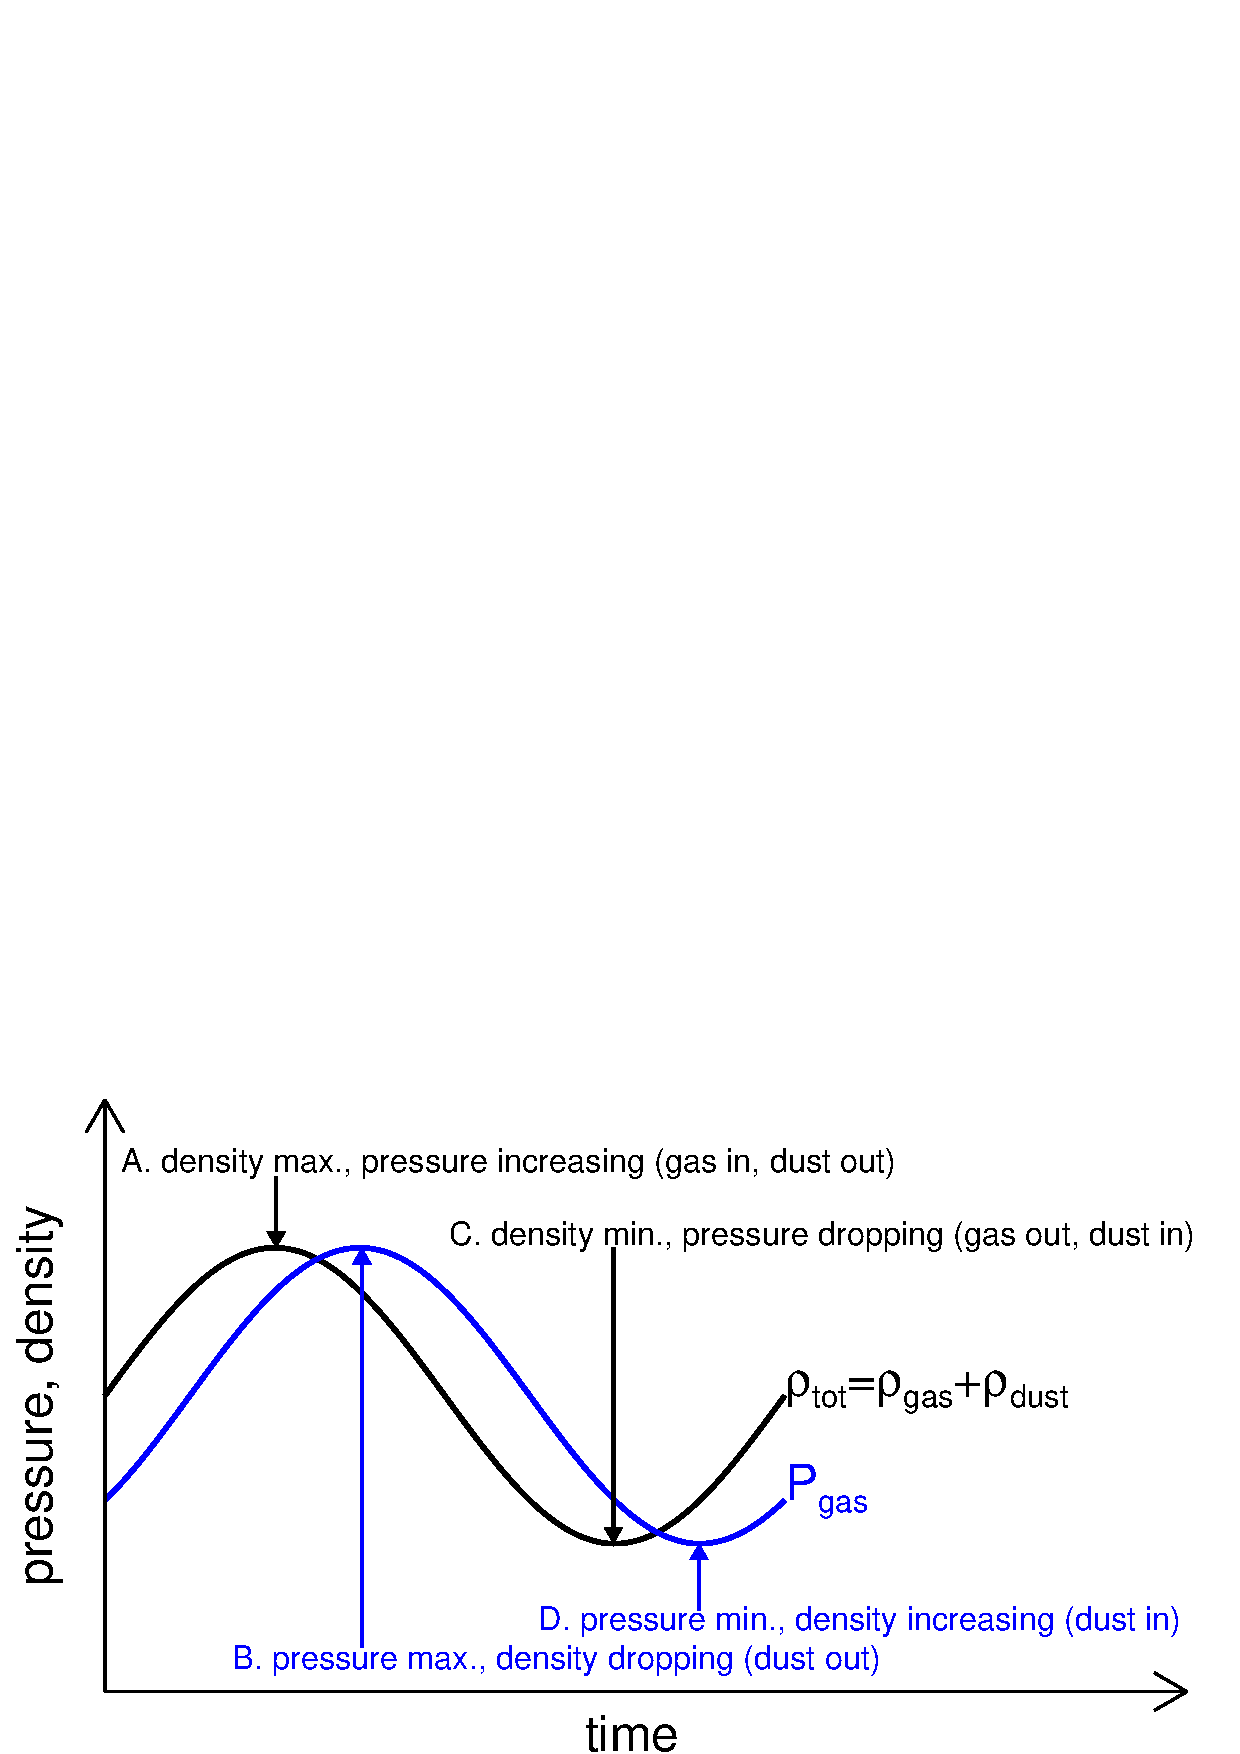
\includegraphics[width=\linewidth]{figures/drag}\\
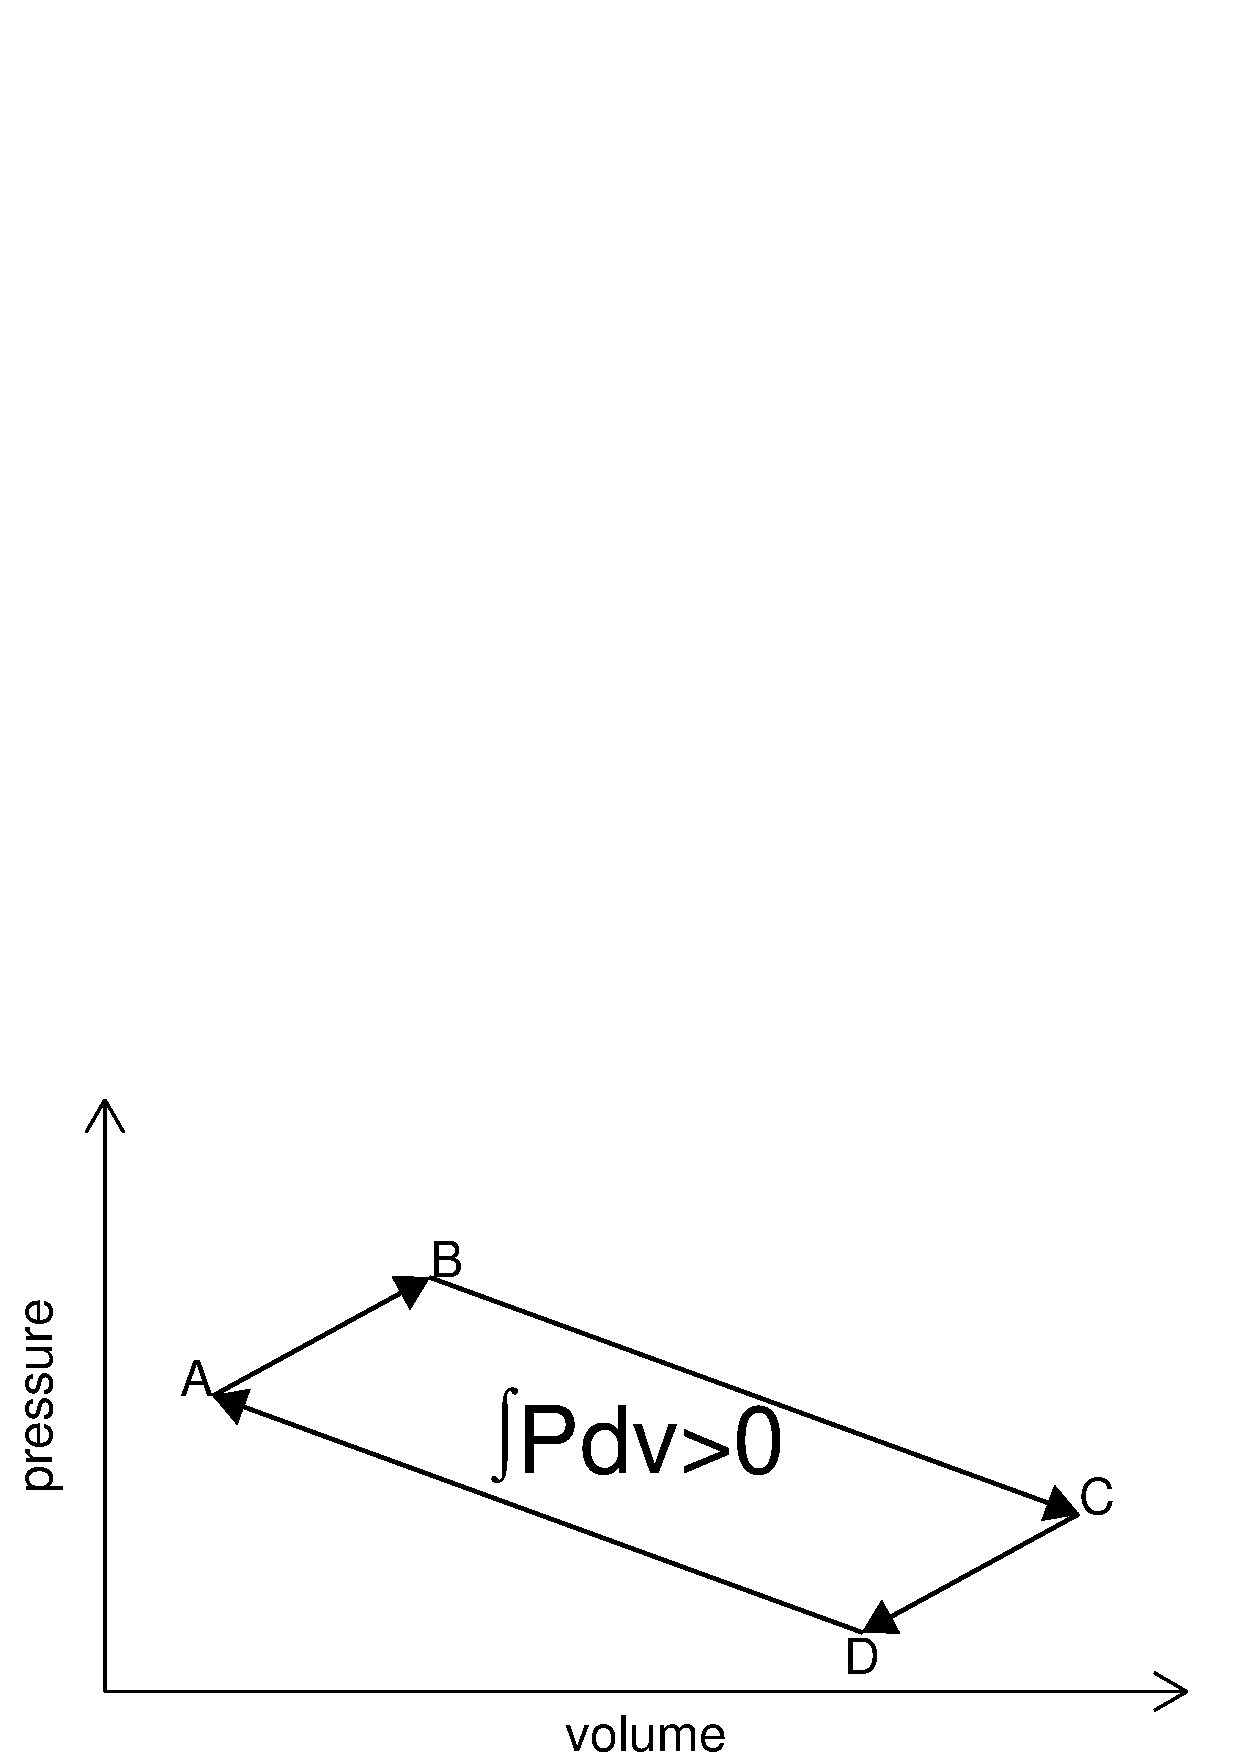
\includegraphics[width=\linewidth]{figures/pdv}
  \caption{Thermodynamic interpretation of growing oscillations in a
    fluid. Top: pressure and density evolution in time. 
    Bottom: oscillation cycle in the P-V plane. In the case shown, 
    dust-drag causes  
    pressure (due to gas only) to lag behind total density. This results in a clockwise path in
    the P-V plane, implying positive work done by the fluid, which 
     would increase oscillation amplitudes.  
    \label{pdv_cartoon}
  }
\end{figure}

There are several situations where the pressure and density of a fluid
are not in phase. The obvious case is if the fluid is subject to
external heating/cooling. For example, in strongly irradiated
protoplanetary disks the
disk temperature  $T(r)$ is time-independent but varies with the cylindrical radius
$r$ from the star \citep{chiang97}. Since $P\propto \rhog T$ for an
ideal gas, %the pressure of a gas parcel varies with  
%position as well. 
there is no reason to expect $P$ and $\rhog$ to 
be in phase as a gas parcel oscillates between different radii and adopt the corresponding local temperatures. 
 In 
fact, we will show that this is a fundamental property of the vertical
shear instability \citep{lin15}.   

%temperature of a fluid parcel changes with position

Another possibility, as annotated in Fig. \ref{pdv_cartoon}, is a dusty gas. The
relevant density here is the total density $\rho = \rhod + \rhog$, 
but the fluid pressure $P$ is due to gas only. If dust were 
perfectly-coupled to the gas, then $P$ and $\rho$ would be in phase, 
and there is no work done. However, for finite dust-gas drag, $\rhod$ and
$\rhog$ are not necessarily in phase, because dust particles can
drift relative to the gas.   
If this causes $P$ to lag 
$\rho$, then the positive work done would lead to growing
oscillations. Indeed, we show that this is true for the streaming
instability. 

In order to apply this thermodynamic interpretation of dust-gas drag
instabilities, we need to develop a formal analogy between dusty-gas
and pure hydrodynamics. We show this is possible in the limit of
strong drag and a fixed gas equation of state. 

\section{Single fluid description of dusty gas}\label{setup} 
We model an accretion disk as a mixture of gas with dust treated as a 
pressureless fluid. We denote their density and
velocity field as $(\rhog,\bm{v}_\mathrm{g})$ and
$(\rhod,\bm{v}_\mathrm{d})$, respectively. The mixture has a single 
temperature $T$, and the mixture pressure $P$ arise solely from the 
gas component.  

The two fluids interact via a drag force parameterized by a stopping
time $\tstop$ 
such that 
\begin{align}  
  \rhod\left.\frac{\p \bm{v}_\mathrm{d}}{\p t}\right|_\mathrm{drag}= -
  \rhog\left.\frac{\p \bm{v}_\mathrm{g}}{\p t}\right|_\mathrm{drag}=
  - \frac{\rhog\rhod}{\left(\rhod+\rhog\right)}\frac{\left(\bm{v}_\mathrm{d} -
    \bm{v}_\mathrm{g}\right)}{\tstop}. 
\end{align}
is the dust-gas friction force per unit volume. Note that $\tstop$ 
differs slightly from the stopping time $\tau_\mathrm{s} =
\tstop\rhog/\left(\rhog+\rhod\right)$ defined in previous studies
\citep[e.g.][]{youdin05a,jacquet11}.   

We consider the limit of tightly-coupled dust particles with 
$\tstop\OmK\ll 1 $, where $\OmK$ is the Keplerian orbital
frequency. This allows us to simplify the problem by using the
`terminal velocity approximation' so that the dust-gas velocity
difference is 
\begin{align}
  \bm{v}_\mathrm{d} - \bm{v}_\mathrm{g} = \frac{\nabla
    P}{\rhog}\tstop, 
\end{align}
\citep{youdin05a,jacquet11}. 

%In the limit of strong dust-gas drag (stopping time $\tstop\to 0$) 
In this limit of strong dust-gas drag, \cite{laibe14} give a single
fluid description of the mixture: 
\begin{align}
  &\frac{D\rho}{Dt} = -\rho\nabla\cdot\bm{v}, \label{masseq}\\ 
  &\frac{D\bm{v}}{Dt} = - \nabla\Phi - \frac{1}{\rho}\nabla  P, \label{momeq}\\ 
  &\frac{D\tepsilon}{Dt} = -\frac{1}{\rho} \nabla \cdot \left(\tepsilon 
  \tstop \nabla P \right),\label{dusteq}\\
  &\frac{D T}{D t} = - \left(\gamma-1\right)T\nabla\cdot\bm{v} +
  \mathcal{H}_\mathrm{drag} + \mathcal{H}_\mathrm{eff}  - \Lambda, \label{tempeq} 
\end{align}
where $D/Dt \equiv \p_t + \bm{v}\cdot\nabla$ is the Lagragian
derivative \emph{following the mixture} with center-of-mass velocity  
\begin{align}
  \bm{v} \equiv \frac{\rhog\bm{v}_\mathrm{g} + 
    \rhod\bm{v}_\mathrm{d}}{\rho}, 
\end{align}
and 
\begin{align}
  \rho \equiv \rhog + \rhod
\end{align}
is the total mixture density. For an ideal gas the pressure is given
by $P = \mathcal{R}\rhog T/\mu $, where $\mathcal{R}$ is
the gas constant and $\mu$ is the mean molecular weight. 

In Eq. \ref{dusteq}, 
\begin{align}
  \tepsilon \equiv \frac{\rhod}{\rho}  = \frac{\epsilon}{1+\epsilon} 
\end{align}
is the dust-fraction and $\epsilon=\rhod/\rhog$ is the usual
dust-to-gas ratio. Note that Eq. \ref{dusteq} is 
equivalent to Eq. 46 of \cite{jacquet11}. 

For the mixture's temperature evolution, Eq. \ref{tempeq}, $\gamma$ is
the adiabatic index; $\mathcal{H}_\mathrm{drag}$ represents heating
due to dust-gas drag and $\mathcal{H}_\mathrm{eff}$ is an effective
energy source arising from transforming from the two-fluid to
one-fluid description \citep[see][ for details]{laibe14}. We also
include a simple model of radiative cooling,
\begin{align}
  \Lambda = \frac{T -
    T_\mathrm{ref}}{t_\mathrm{cool}}, \label{realenergy} 
\end{align}
which relaxes the mixture back to a prescribed temperature profile   
$T_\mathrm{ref}$ on a timescale of $\tcool$. We will shortly simplify
the problem by considering rapid cooling, $\tcool\to0$. 


For the disk problem the external potential $\Phi$ is  
that for a star of mass $M_*$, 
\begin{align}\label{thin_disk_potential}
  \Phi(r,z) =-\frac{GM_*}{\sqrt{r^2 + z^2}}\simeq
  -\frac{GM_*}{r}\left(1 - \frac{z^2}{2r^2}\right), 
\end{align}
where $G$ is the gravitational constant, and $(r,\phi, z)$ are
cylindrical co-ordinates centered on the star. 
The second equality is the 
thin-disk approximation for the disk potential, appropriate for
$|z|\ll r$. We shall adopt this approximate potential in order to
obtain analytic expressions for the disk equilibria.  

\subsection{Locally isothermal equation of state}\label{loc_iso_eos}
For later comparison it is convenient to re-write the temperature
evolution, Eq. \ref{tempeq}, to that for the pressure: 
\begin{align}
  \frac{\p P}{\p t} + \bm{v}_\mathrm{g}\cdot\nabla P = - \gamma P
  \nabla\cdot \bm{v}_\mathrm{g}  + \mathcal{H} 
%\frac{\rho \mathcal{R}}{\mu}\frac{T
%  - T_\mathrm{ref}}{t_\mathrm{cool}}, \label{realenergy}
\end{align}
where $\mathcal{H}$ collects together dust-drag heating and radiative
cooling. 

We now simplify the gas energy equation by considering short cooling 
times $\tcool\to 0$, appropriate for the outer parts of an irradiated
protoplanetary disk \citep{chiang97,lin15}. Then the disk temperature
$T = T_\mathrm{ref}$ at all times, and so we may
adopt a locally isothermal equation of state 
\begin{align}\label{eos}
  P = c_s^2(r,z)\rhog = c_s^{2}(1 - \tepsilon)\rho,   
\end{align}
where $c_s(r,z)= \sqrt{\mathcal{R}T_\mathrm{ref}/\mu}$ is a prescribed
sound-speed profile fixed in time.  

In practice we consider vertically 
isothermal disks with \begin{align}\label{power_temp}
  c_s^2(r) \propto r^{q},
\end{align}
where $q$ is the power-law index for the disk temperature. For $q=0$
the disk is strictly isothermal. 

If we define the effective sound-speed $c_{s,\mathrm{eff}} = c_s\sqrt{\left(1 -
    \tepsilon\right)}$, then the equation of state has the standard
form $P=c_{s,\mathrm{eff}}^2\rho$. Since the dust-fraction $\tepsilon$
typically decrease away from the midplane, we expect vertically
isothermal dusty disks to in fact behave as if it
had a temperture \emph{increasing} away from $z=0$.   

\subsection{Effective energy equation}
Although we have eliminated the need of an evolutionary energy
equation (Eq. \ref{realenergy}) by choosing a locally isothermal
equation of state (Eq. \ref{eos}), we show that the mixture 
nevertheless obeys an effective evolutionary energy equation. This is
because advection of the dust-fraction, described by
Eq. \ref{dusteq}, can be transformed into an energy-like 
equation. We 
%We show that for a prescribed temperature distribution, the mixture
%obeys an evolutionary energy equation, due to the advection of the
%dust-fraction. 
eliminate $\tepsilon$ in favor of $P$, 
\begin{align*}
  \tepsilon = 1 - \frac{P}{c_s^2(r,z)\rho}, 
\end{align*}
then Eq. \ref{dusteq} becomes
\begin{align}
%\frac{DP}{Dt} 
\frac{\p P}{\p t} + \bm{v}\cdot\nabla P  
&= - P \nabla\cdot\bm{v} + P\bm{v}\cdot\nabla\ln{c_s^2}
                + \mathcal{C},  \label{eff_energy} \\
\mathcal{C}&\equiv c_s^2 \nabla\cdot\left[\tstop\left(1 -
  \frac{P}{c_s^2\rho}\right)\nabla 
  P\right].
\end{align}
Comparing with Eq. \ref{realenergy}, we see that 
Eq. \ref{eff_energy} is the energy equation for an ideal gas of
adiabatic index $\gamma=1$, but now with the imposed temperature
gradient $\nabla c_s^2$ and dust-gas drag $\mathcal{C}$ playing the
role of radiative cooling ($\Lambda$ in 
Eq. \ref{realenergy}). 

%In this form, the function $\mathcal{C}$ can be interpreted
%as a cooling term.    
If we denote 
\begin{align}
  \bm{F} \equiv  - \frac{\nabla P}{\rho}
\end{align}
for the pressure forces, then
\begin{align*}
  \mathcal{C} = - c_s^2\nabla \left( \tepsilon \tstop \rho \bm{F}
  \right), 
\end{align*}
which is in the same form as cooling by radiative diffusion. In protoplanetary
disks the heat flux, proportional to $\bm{F}$, is directly radially
outwards and vertically upwards. This is simply a reflection of
particle drift (inwards and downwards). Particle flux into a region contributes
to `cooling' of that region because the effective temperature is
lowered. 

Eq. \ref{eff_energy} can be written in conservative form,
\begin{align*}
  \frac{\p P}{ \p t} + \nabla\cdot\left\{P\left[\bm{v} -
      \tstop\left(c_s^2 - \frac{P}{\rho}\right)\nabla\ln{P}\right]
    \right\}\\
  = \left[P\bm{v} - \tstop\left(c_s^2 - \frac{P}{\rho}\right)\nabla
    P\right]\cdot\nabla\ln{c_s^2}. 
\end{align*} 
We may thus re-interpret $P$ as the mixture's energy density, but the
energy flux has an additional contribution from the pressure
gradient and dust-gas friction. The term on the right-hand-side, owing
to the imposed temperature profile, can be interpreted as an external
heat source.  

%We comment that 

\subsection{Entropy of an isothermal dusty gas }

The gas component of the mixture has a specific entropy
$S = C_p\ln{\left(P^{1/\gamma}/\rhog\right)}$, where $C_p$ is the heat capacity at constant
pressure. However, this is not a useful quantity for (locally)
isothermal gas. 

Nevertheless, since we have shown that an isothermal dusty gas
effectively has $\gamma=1$ we can define an effective (dimensionless)  
entropy for the \emph{entire mixture} as 
\begin{align}
   \seff \equiv \ln \frac{P}{\rho} = \ln{\left[c_s^2(1-\tepsilon)\right]}.  
\end{align} 
We shall see that by defining an effective entropy this way, many of the 
results concerning the stability of dusty gas will have identical form
and interpretations to that in standard adiabatic hydrodynamics of 
pure gas. For example, if $c_s^2$ is constant and $\tstop=0$, then
$D\seff/ D t = 0$ since $D\tepsilon/D t=0$ in that case.  

The physical reason for this analogy is that with strong drag, the dust is almost
perfectly entrained in the gas flow, but there is some gain/loss of 
dust particles between different gas parcels if dust-gas
friction if finite. This property is analogous to the entropy of an adiabatic
pure gas subject to heating/cooling: entropy is conserved following
a gas parcel, except if there is heat exchange between a fluid parcel
and the surrounding.  

\section{Dynamical equilibria}\label{eqm}
 
For a given distribution of the dust-fraction $\tepsilon$ (or
dust-to-gas ratio $\epsilon$), the 
mass and momentum Eqs. \ref{masseq}---\ref{momeq} admit     
axisymmetric steady states with $\rho(r,z)$ and 
$\bm{v}=r\Omega(r,z)\hat{\bm{\phi}}$ where $\Omega = v_\phi/r$, which satisfy 
\begin{align}
  r\Omega^2 &= \frac{\p \Phi}{\p r} + \frac{1}{\rho}\frac{\p P}{\p
    r},\label{steady_momr}\\
  0 & = \frac{\p\Phi}{\p z} + \frac{1}{\rho}\frac{\p P}{\p z},\label{steady_momz}
%  0 & = \nabla\cdot\left(\tepsilon\tstop\nabla P\right) \label{steady_dust}
\end{align}
with $P=P(\tepsilon,\rho)$ given by the equation of state
(Eq. \ref{eos}). An explicit solution is presented in
\S\ref{steady_state}.  
However, disk structures obtained this way generally do not satisfy 
the steady state effective energy Eq. \ref{eff_energy} because
$\mathcal{C}\neq0$ for general solutions to
Eq. \ref{steady_momr}---\ref{steady_momz}. 

In practice the dust particles settle vertically on a timescale 
$t_\mathrm{settle}\sim 1/\OmK^2\tstop$, although for tightly-coupled dust
particles this is much longer than that to establish vertical
hydrostatic equilibrium in the gas component ($\sim 1/\OmK$).  
True steady states may be calculated by invoking an underlying gas
turbulence, which leads to dust diffusion \citep{takeuchi02, youdin07, 
 lyra13}. This complication is beyond the scope of this paper. 

In this work, we will assume that $\tstop$  is sufficiently small so
that settling occurs on much longer timescales  than that of interest; or
consider equilibria with $\mathcal{C}\equiv 0$, namely   
\begin{inparaenum}[1)] 
\item 
  unstratified disks with finite dust-gas drag (\S\ref{si});  
\item 
  perfectly-coupled dust with $\tstop=0$ (\S\ref{results}). 
\end{inparaenum} 
Vertical settling is absent in both cases. 


%Eq. \ref{steady_dust} makes it difficult to obtain equilibrium
%solutions explicitly. However, if the diffusive process is slow and
%can be neglected, then one may just solve
%Eq. \ref{steady_momr}---\ref{steady_momz} with a prescribed (initial)
%distribution of the dust fraction $\tepsilon(r,z)$. 

\subsection{Disk structure with a prescribed dust distribution}\label{steady_state}  
To obtain an actual disk structure for numerical computations, we
assume a Gaussian profile in the dust-to-gas ratio,   
\begin{align}\label{dust_gauss}
  \epsilon(r,z) = \epsilon_0(r)
  \exp{\left[-\frac{z^2}{2\Htilde^2(r)}\right]}. 
\end{align}
%For simplicity we assume the dust-to-gas ratio at the mid-plane
%$\epsilon_0$, as well as its characteristic scale-height
%$\widetilde{H}$, are both constant.
% We take the mid-plane dust-to-gas ratio
%to be a power-law in radius,  
%\begin{align}
%  \epsilon_0(r) = \epsilon_{00}\left(\frac{r}{r_0}\right)^{-d},  
%\end{align}
%where $\epsilon_{00}$ is the dust-to-gas ratio at the fiducial radius
%$r_0$.  
Inserting Eq. \ref{dust_gauss} into vertical hydrostatic equilibrium,
Eq. \ref{steady_momz} and integrating with the approximate
gravitational potential (Eq. \ref{thin_disk_potential}) we obtain the
gas density as
\begin{align}
  &\rhog(r,z)= \notag\\
&\rho_\mathrm{g0}(r)\exp{\left\{ - \frac{z^2}{2\Hgas^2}
    -\epsilon_0\frac{\Htilde^2}{\Hgas^2}\left[1 -
      \exp{\left(-\frac{z^2}{2\Htilde^2}\right)}\right] \right\}}, 
\end{align}
where
\begin{align}
  \Hgas = \frac{c_s}{\OmK}, \quad \OmK \equiv \sqrt{\frac{GM_*}{r^3}},   
\end{align}
is the gas scale-height in the dust-free limit and $\OmK$ is the
Keplerian frequency, respectively. 

We usually consider gas-dominated disks with $\epsilon_0 \ll 1$.  
Then $\rhog(r,z)$ is effectively Gaussian, as in the 
dust-free case. The dust density is approximately 
\begin{align}
  \rhod \simeq \epsilon_0\rho_\mathrm{g0}(r) \exp
        {\left(-\frac{z^2}{2H_\mathrm{d}^2}\right)}, 
\end{align}
with 
\begin{align}
  \frac{1}{H_\mathrm{d}^2} = \frac{1}{\Htilde^2} + \frac{1}{\Hgas^2}, 
\end{align}
and $H_\mathrm{d}$ is the dust-scale height. In numerical
calculations, we  we specify $H_\mathrm{d}< \Hgas$ to obtain 
$\Htilde$ for input. 

Finally, we define 
\begin{align}
  Z \equiv \epsilon_0\frac{\Hd}{\Hg} \simeq
  \frac{\Sigma_\mathrm{d}}{\Sigma_\mathrm{g}} 
\end{align}
as a measure of the local metalicity, where $\Sigma_\mathrm{d}$ and
$\Sigma_\mathrm{g}$ are the dust and gas surface densities,
respectively. The second equality holds for $\epsilon_0\ll1$.  

%\Sigma_\mathrm{d}$ and the gas
%surface density $\Sigma_\mathrm{g}$.  

\subsection{Orbital frequency} 
In the thin-disk approximation, the disk orbital frequency is 
\begin{align}
  \Omega(r,z) = \OmK(r)\left[1 - \frac{3}{2}\frac{z^2}{r^2} +
    \frac{h_\mathrm{g}^2}{\left(1+\epsilon\right)}\frac{\p}{\p\ln{r}}\ln{\left(c_s^2\rhog\right)}
    \right]^{1/2}, 
\end{align}
where 
\begin{align}
  h_\mathrm{g} \equiv \frac{\Hgas}{r}
\end{align}
is the characteristic disk aspect-ratio. 

\subsection{Vertical shear}\label{vertshear}
The mixture possess vertical shear. To see this, we eliminate $\Phi$
between Eq. \ref{steady_momr}---\ref{steady_momz} to 
obtain 
\begin{align}\label{vshear}
  r\frac{\p \Omega^2}{\p z} 
%&= \frac{\p\ln{\rho}}{\p r}\frac{\p}{\p
%    z}\left[c_s^2(1-\tepsilon)\right] - \frac{\p\ln{\rho}}{\p z}
%  \frac{\p}{\p r} \left[c_s^2(1-\tepsilon)\right]\\  
   = \frac{1}{\rho}\left(\frac{\p P}{\p r}\frac{\p \seff}{\p z} -\frac{\p
    P}{\p z}\frac{\p \seff}{\p r} \right). 
\end{align}
Writing Eq. \ref{vshear} in terms of the gas density and dust-to-gas
ratio with a power-law temperature profile (Eq. \ref{power_temp}) gives 
\begin{align}\label{vshear2}
  &r\frac{\p \Omega^2}{\p z}  =
  \frac{c_s^2(r)}{\left(1+\epsilon\right)^2}\left\{
  \frac{\p\epsilon}{\p r}\frac{\p\ln{\rhog}}{\p z}
%  -\frac{\p\epsilon}{\p z}\left[\frac{\p\ln{\rhog}}{\p r} + \frac{q}{r}\right]\right.\notag\\
 -\frac{\p\epsilon}{\p z}\frac{\p\ln{P}}{\p r}\right.\notag\\
  &\phantom{ r\frac{\p \Omega^2}{\p z}  =
    \frac{c_s^2(r)}{\left(1+\epsilon\right)^2}\left\{\right\} }
  \left. -\frac{q}{r} \left(1+\epsilon\right)\frac{\p\ln{\rhog}}{\p z} \right\} 
\end{align}
The first two terms correspond to vertical shear caused by spatial
variations in the dust-to-gas ratio; while the third term
proportional to $q$ corresponds to vertical shear due to the 
radial temperature gradient. The last term survives in the dust-free
limit. 

We can compare these sources by 
evaluating them using the equilibrium
solutions in \S\ref{steady_state}. We assume the disk is radially
smooth so that $\p_r\sim 1/r$, and the dust-to-gas ratio
$\epsilon\ll1$. This gives 

\begin{align}\label{vshear_split}
  \frac{\left|r\p_z\Omega\right|_{\text{
        dust/gas gradient}}}{\left|r\p_z\Omega\right|_{\text{
        temp. gradient}}} \sim
 % \epsilon \frac{\mathrm{max}\left(\delta^2,
  %  1\right)}{\left|q\right|\left(\epsilon + \delta^2\right)},
 \epsilon \frac{\mathrm{max}\left(\delta^2,
    1\right)}{\left|q\right|\left(1+\epsilon\right)\delta^2},
\end{align}
where $\delta\equiv \Htilde/\Hgas$. 
Since $|q|=O(1)$ in PPDs, Eq. \ref{vshear_split} indicates that
vertical shear due to variations in the dust-to-gas ratio dominates 
over that due to the radial temperature gradient for thin dust layers
such that $\delta^2\ll \epsilon$. Otherwise, vertical shear is
associated with $\p_rc_s^2$.  

\subsection{Vertical buoyancy}\label{vbuoyancy}
Having identified the entropy of an isothermal dusty gas, we find the
vertical buoyancy frequency $N_z$ of the mixture is given by 
\begin{align}
  N_z^2 \equiv - \frac{1}{\rho}\frac{\p P}{\p z}\frac{\p \seff}{\p z} &=
  \frac{c_s^2(r)}{\left(1+\epsilon\right)^2}\frac{\p\ln\rhog}{\p 
  z}\frac{\p\epsilon}{\p z} \\ &
                                  =
  \frac{\epsilon}{\left(1+\epsilon\right)^2}\left(\frac{z}{\Htilde}\right)^2\OmK^2\notag,  
\end{align}
where the second equality assumes $c_s=c_s(r)$ and the final equality
applies to the equilibria in \S\ref{eqm}. Thus,  
\begin{align*}
N_z\lesssim
O\left(\sqrt{\epsilon_0}\OmK\right). 
\end{align*}
However, for thick dust layers such that $H_\epsilon \gg \Hg$, 
$\mathrm{max}\left(N_z\right)$ may occur outside a finite vertical domain.  


 % N_z^2 
%\end{align}

\section{Limiting behaviours}\label{limits}

In this section we review the basic properties of the 
single-fluid mixture using Eqs.\ref{masseq}--\ref{momeq} with 
Eq. \ref{eff_energy} in place of the dust continuity equation. Our
discussion is based on the corresponding axisymmetric linearized
equations. A variable $f$ is
subject to Eulerian perturbations of the form 
\begin{align}
 \real\left[ \delta f(r,z)\exp{\left(-\ii\sigma t\right)}\right], 
\end{align}
where $\sigma$ is the complex mode frequency. For later convenience we
write 
\begin{align}
  \sigma = \ii s - \omega,
\end{align}
where $s$ and $\omega$ are the growth rate and real frequencies,
respectively. Thus perturbations have time dependence $e^{st +
  \ii\omega t}$.  

In Appendix
\ref{var_prin} we derive the integral relation,  
\begin{align}
%&  \sigma^2\int\rho\left(|\dd v_r|^2 + |\dd v_z|^2\right)dV \notag\\
  \sigma^2\mathcal{I}^2
&= \int\left[ \rho
  |\dd v_r|^2A + \rho  \dd v_z \dd v_r^* B + \rho \dd v_z^*\dd v_r C +
  \rho |\dd v_z|^2 D\phantom{\frac{1}{1}}\right. \notag\\
&\phantom{===}  \left. + \frac{1}{P}\Bigl\lvert \nabla\cdot\left(P\dd
  \bm{v}\right)\Bigr\rvert^2\right]dV  -\int \left(\nabla\cdot\dd\bm{v}^*\right)\dd\mathcal{C}dV \notag\\
&\phantom{===}
- \int P
  \left(\nabla\cdot\dd\bm{v}^*\right)\left(\dd\bm{v}\cdot\nabla\ln{c_s^2}\right)dV.\label{int_rel}
\end{align} 
The real integral $\mathcal{I}^2>0$ and coefficients $A,B,C,D$ can be
read off Eq. \ref{integral_ex}. %Note that $B=C$ from dynamical equilibrium
%(Eq. \ref{vshear}). 
We now consider various limits of Eq. \ref{int_rel}.    


\subsection{Strictly isothermal gas perfectly coupled to dust}\label{iso_perfect}
When $c_s^2$ is a constant and $\tstop=0$, the dusty-gas equations are
exactly equivalent to that for adiabatic hydrodyamics with unit adiabatic
index. Although the gas is strictly isothermal, the mixture behaves 
adiabatically because the dust fraction $\tepsilon$ is advected with 
the gas. This is similar to entropy being conserved following an
adiabatic gas when there is no heating or cooling.  

In this case, the last two integrals in Eq. \ref{int_rel} vanish. Then 
requiring $\sigma^2>0$  gives the criteria 
for the axisymmtric \emph{stability} of an isothermal gas perfectly 
coupled to dust,  
\begin{align}
  \kappa^2 + c_s^2 \nabla\ln{\rhog}\cdot\nabla\tepsilon &> 0,\label{dusty_solberg1}  \\
  -c_s^2\frac{\p\ln{\rhog}}{\p z}\left(-\kappa^2\frac{\p\tepsilon}{\p
    z} + r\frac{\p\Omega^2}{\p z}\frac{\p \tepsilon}{\p r} \right) & > 0, \label{dusty_solberg2}
\end{align} 
%\begin{align}
%  \kappa^2 - \frac{1}{\rho}\nabla P \cdot \nabla s &> 0, \label{dusty_solberg1}    \\
%  -\frac{1}{\rho}\frac{\p P}{\p z} \left(\kappa^2 \frac{\p s}{\p z} -
%  r\frac{\p\Omega^2}{\p z}\frac{\p s}{\p r}\right) &>0, \label{dusty_solberg2}
%\end{align} 
where %$s = \ln{P/\rho}$, 
$\kappa^2 \equiv r^{-3}\p_r\left(r^4\Omega^2\right)>0$ is the 
square of the epicylic frequency. %We assume $\kappa^2>0$.  
Eq. \ref{dusty_solberg1}---\ref{dusty_solberg2} are in fact the 
the Solberg-Hoiland criteria for axisymmetric stability of adiabatic
gas if one inserts $C_p\ln{\left(1 -
    \tepsilon\right)}$ for the entropy in the standard
expression for said criteria \citep[e.g.]{tassoul78}.   


\subsubsection{Order-of-magnitude estimates} 
We evaluate the above stability criteria for the vertically-Gaussian
distributions for the gas density and the dust-to-gas ratio as 
described in \S\ref{eqm}. 
%However, here we permit 
%$\epsilon_0=\epsilon_0(r)$ and $\Htilde=\Htilde(r)$ to vary with
%radius. 
We assume the disk is approximately Keplerian so that
$\kappa\simeq\OmK$. In terms of the dust-to-gas
ratio $\epsilon$, Eq. \ref{dusty_solberg1}---\ref{dusty_solberg2}
become   
\begin{align}
  &1 + \frac{\epsilon}{\left(1+
    \epsilon\right)^2}\left(h_\mathrm{g}^2\frac{\p\ln{\rhog}}{\p\ln{r}}
  \frac{\p\ln{\epsilon}}{\p\ln{r}} + 
  \frac{z^2}{\Htilde^2}\right)>0 \label{stability_est1},   \\ 
&1 - \frac{\epsilon
  h_\mathrm{g}^2}{\left(1+\epsilon\right)^2}
  \frac{\p\ln{\epsilon}}{\p\ln{r}}\left(-\frac{\p\ln{\rhog}}{\p\ln{r}}+\frac{\Htilde^2}{H_\mathrm{g}^2}\frac{\p\ln{\epsilon}}{\p\ln{r}}\right)
  > 0 \label{stability_est2},
\end{align}
\emph{for stability}. 

Eq. \ref{stability_est1}---\ref{stability_est2} are easily satisfied
in thin accretion disks where radial gradients are $O(1/r)$, 
$h_\mathrm{g}\ll 1$ and $\Htilde/H_\mathrm{g}$ not too
large.  Then the
magnitude of the second term on the left-hand-side  of either
inequality is much less than unity. Thus radially smooth, strictly
isothermal disks perfectly coupled with dust are stable against
axisymmetric perturbations.  

%Such disks are stable against
%axisymmetric perturbations.  

\subsubsection{Instability at dust edges}
Notice the left-hand-side of Eq. \ref{stability_est2} is a quadratic in
$\p_r\epsilon$. It is possible to
violate this inequality for sufficiently large (in magnitude) radial
gradients  in the dust-to-gas ratio, 
\begin{align}
  \frac{\p\ln{\epsilon}}{\p\ln{r}} > S_+ \quad \mathrm{or} \quad 
  \frac{\p\ln{\epsilon}}{\p\ln{r}} < S_-,
\end{align}
\emph{for instability}, where
\begin{align}\label{spm}
S_\pm = \frac{1}{2}\frac{H_\mathrm{g}^2}{\Htilde^2} 
  \left[
  \frac{\p\ln{\rhog}}{\p\ln{r}} \pm 
  \sqrt{
  \left(\frac{\p\ln{\rhog}}{\p\ln{r}}\right)^2 + 
  4 \frac{\Htilde^2}{H_\mathrm{g}^2}
  \frac{\left(1+\epsilon\right)^2}{\epsilon h_\mathrm{g}^2}
  }
  \,\right]. 
\end{align} 
In typical accretion disks where $\p_r\rhog<0$, it is easier to
achieve instability at a given radius for increasing dust-to-gas
ratios in outwards ($\p_r\epsilon > 0$), and vice versa.  

We can neglect density gradients in Eq. \ref{spm} 
if $r\p_r\ln{\rhog}\sim O(1)$ and $H_\epsilon/\Hgas\gg
\sqrt{\epsilon}\hgas$. For example, if $\epsilon\simeq 0.01$ and
$\hgas\simeq 0.05$, then we require $H_\epsilon/\Hg\gg
5\times10^{-3}$. (So the dust layer thickness $\Hd\gg 5
\times10^{-3}\Hgas$ as well.) Then 
instability requires 
\begin{align}\label{dust_edge}
\left|\frac{\p\ln{\epsilon}}{\p r}\right| \gtrsim
  \frac{1}{\Htilde}\frac{\left(1+\epsilon\right)}{\sqrt{\epsilon}}.
%\simeq
 % \frac{1}{\sqrt{\epsilon}H_\epsilon}, 
\end{align}
%where the second equality applies to $\epsilon\ll 1$. 
That is, if the radial lengthscale of the dust-to-gas ratio,
$L_\epsilon\ll O(\Htilde)$, i.e. its vertical lengthscale,  
then the system is potentially unstable.  

Taking $\epsilon\sim 0.01$,  we find that 
for thin dust layers with $H_\epsilon \simeq \Hd\ll \Hg$,  instability
requires $L_\epsilon\ll O(0.1\Hg)$, i.e. the dust-to-gas ratio must
vary on an extremely short lengthscale. 
%an extremely short  
%radial length-scale in the dust-to-gas ratio. 
This is unlikely to
occur. On the other hand, if dust is well-mixed, say $\Hd\simeq
0.99\Hg$, then instability only requires 
$L_\epsilon\lesssim O(10\Hg)$, which is more realistic. 

%This is responsible for 
%the usual vertical shear instability in locally isothermal disks.
%However, we may obtain an integral
%relation for linear, axisymmetric waves with frequency $\sigma$ (see
%Appendix \ref{var_prin}, where we also account for finite $\tstop$) in
%the form:   
%If $c_s$ is constant, then $\sigma^2$ is real, and 
%the first integral leads to the previous Solberg-Hoiland criteria for 
%axisymmetric stability. However, when $c_s$ is non-uniform, 

\subsection{Thermodynamics of dust-drag instabilities}\label{dust_work}
Now consider constant $c_s$ but $\tstop\neq0$. 
Eq. \ref{int_rel} indicates that $\sigma^2$ is generally complex, so
we may have growing oscillations (overstability). %Writing $\sigma =
%-\omega + \ii s$ where $\omega$ and $s$ are the real frequency and
%growth rates, respectively, 
The imaginary part of Eq. \ref{int_rel}
gives  
\begin{align}
%  s = \frac{\imag\int \left(\nabla\cdot\dd\bm{v}^*\right)\dd\mathcal{C}dV}{2\omega\int\rho\left(|\dd
%    v_r|^2 + |\dd v_z|^2\right)dV}, \label{thermal_instability}
  s = \frac{\imag\int \left(\nabla\cdot\dd\bm{v}^*\right)\dd\mathcal{C}dV}{2\omega\mathcal{I}^2}. \label{thermal_instability}
\end{align} 
This represents instability due to dust-gas friction. 
Since drag ($\delta \mathcal{C}$) appears as a source term in our
effective energy equation, the quantity 
$\imag\left[\left(\nabla\cdot\dd\bm{v}^*\right)\dd\mathcal{C}\right]$
may be thought of as a correlation between compression/expansion and  
heating/cooling.  

It is well-known that such correlations can lead to pulsational
instabilities in stars \citep{cox67}. We thus interpret  
dust-drag instabilities in a similar way, 
adapting from the treatment of stellar 
pulsations by \cite{cox67} and lecture notes by \cite{samadi15} and 
J. Christensen-Dalsgaard\footnote{\url{http://astro.phys.au.dk/$\sim$jcd/oscilnotes/}}.      

%and disks
%\cite{kato78}. 


\subsubsection{Work done by dusty gas} 

The physical interpretation of Eq. \ref{thermal_instability} is that 
work done by pressure forces in the dusty gas leads to growth in
oscillation amplitudes. To see this, we first compute the work done
assuming periodic oscillations. We then show that if the work done is positive, then the
oscillation amplitude in fact grows: the work done leads the
system to `overshoot' past the amplitude of the preceeding oscillation
cycle. 

%its equilibrium. {\bf should be overshoot the max displacement}

The average rate of work done is 
\begin{align}
  \mathcal{W} = \frac{1}{T_p}\int^{t+T_p}_{t}dt^\prime\int_M P
  \frac{D\upsilon}{Dt^\prime} dm \label{work_def} 
\end{align}
\citep{cox67}, 
where $T_p$ is the oscillation period, $\upsilon=1/\rho$ is the specific
volume of the mixture, and the spatial integral is taken over the
total mass $M$ of the mixture and $dm$ is the mass element. 
Noting that only products of perturbations contribute to
$\mathcal{W}$, we find that for periodic oscillations (time dependence 
$e^{\ii\omega t}$ and real $\omega$): 
\begin{align}
  \mathcal{W} = - \frac{\omega}{2} \int \imag\left(\Delta P
  \frac{\Delta \rho^*}{\rho}\right)dV,\label{work_real}
\end{align}
where %the integral is taken over the volume of the
%mixture; and 
 the Lagragian perturbation $\Delta$ of a variable $f$ is 
$\Delta f = \delta f + \bm{\xi}\cdot\nabla f$; where $\bm{\xi}$ is the
Lagragian displacement ($    \xi_{x,z} =  \ii \dd v_{x,z}/\sigma$).  
Eq. \ref{work_real} show that a phase difference between gas pressure and
the total density leads to work done
($\mathcal{W}\neq0$).  

Now, quite generally, Eq. \ref{lin_mass_full}---\ref{lin_energy_full} 
imply the integrand of the numerator in Eq. \ref{thermal_instability} 
is 
\begin{align} 
  \imag \left(\delta \mathcal{C}
  \nabla\cdot\dd \bm{v}^*\right) = 
  -|\sigma|^2\imag \left(\Delta P 
  \frac{\Delta\rho^*}{\rho}\right). \label{pdv}
\end{align}
%This states that `PdV' work (the right-hand-side) is 
%provided by dust-drag friction, and can be seen explicitly as 
%follows. 
Then combining Eq. \ref{work_real}, \ref{pdv} and
\ref{thermal_instability} 
gives  
\begin{align}
s = \frac{\mathcal{W}}{\mathcal{I}^2}, \label{growth_work}
\end{align}
where we have set $\sigma= - \omega$ in 
Eq. \ref{pdv}. Eq. \ref{growth_work} states that if the average work
done is positive during a periodic oscillation, $\mathcal{W}>0$, then
then its amplitude would actually grow ($s>0$).  %and not be periodic 

Positive work done is done by a parcel if $-\omega \imag\left(\Delta  
P\Delta\rho^*\right)>0$. Without loss of generality, take $\omega>0$
and consider a mass element with $\Delta\rho = 1$. Then positive work 
requires $\imag\left(\Delta
P\right)<0$.  This corresponds to pressure perturbations \emph{lagging}
behind that in density (or displacements), since the phase of
the assumed perturbations increase in time.  


Fig. \ref{pdv_cartoon} gives a graphical demonstration that 
if gas pressure lags behind density, then %positive work done 
$\mathcal{W}>0$ because it leads to a clockwise path in the
`P-V' plane. From $A$ to $B$, a fluid parcel is expanding to return to 
equilbrium, but pressure (i.e. restoring) forces is still
increasing. This over-compensation causes the parcel to expand
beyond the maximum volume of the previous cycle. 
%{\bf should be: expand beyond the max
%  vol of the previous cycle}
%corresponds to positive work done. 
Similarly, from $C$ to $D$ the parcel is already contracting towards
equilibrium, but pressure
forces are still dropping. This allows the  
parcel's contraction to over-shoot the maximum density attained in the
previous cycle. 
% {\bf
  %should be contract beyond the min vol of prev cycle}
The 
overall positive work done leads to growth in the oscillation amplitude. 




%$\imag\left(\Delta\rho\right)=0$.   

\subsubsection{Physical picture of dust-gas drag instabilities} 

%We now use physical arguments to show that $\mathcal{W}>0$ if pressure
%perturbations (from the gas) lags behind the total density of the gas
%plus dust mixture. 
%The full energy equation is  
%\begin{align*}
%  \frac{DP}{Dt} = \frac{P}{\rho}\frac{D\rho}{D t} + \mathcal{C}. 
%\end{align*} 
%Dust-drag causes a phase difference between the pressure and density 
%evolution of a fluid element. 

%Consider a fluid element at maximum density during an
%oscillation cycle (point $A$), so that $D\rho/ D t = 0$. If dust-gas
%drag provides an effective heating to the fluid element at $A$
%(i.e. gas influx)  then it will experience increasing pressure, $DP/D
%t>0$. It attains pressure maximum (point $B$) \emph{after} reaching
%density maximum. 

%Applying the above argument to isothermal dusty gas, 
For dusty gas, the work done during oscillations 
 is attributed to finite dust-gas drag. The relative
drift between gas and dust causes a phase difference between the two
components. 

A parcel of the isothermal dusty-gas mixture does 
postive work if  
\begin{align*}
-\sgn\left(\omega\right)\imag\left(\Delta\rhog\Delta\rhod^*\right)>0,
\end{align*}
meaning that gas follows dust. Instabilities are thus not possible if the
gas does not respond to dust-drag (i.e. no back-reaction). The
pressure-density lag shown in Fig. \ref{pdv_cartoon} is achieved if, 
after a parcel reaches maximum total density, its 
gas content is still increasing ($A$ to $B$). This in turn implies a sufficiently
large particle flux \emph{out} of the parcel.   

{\bf lagrangian derivative follows the mixture. this highlights one
  perk of the one-fluid framework. in two-fluid models there are two
  types of lagragian deriv, not clear which fluid to follow.}

\begin{figure}
  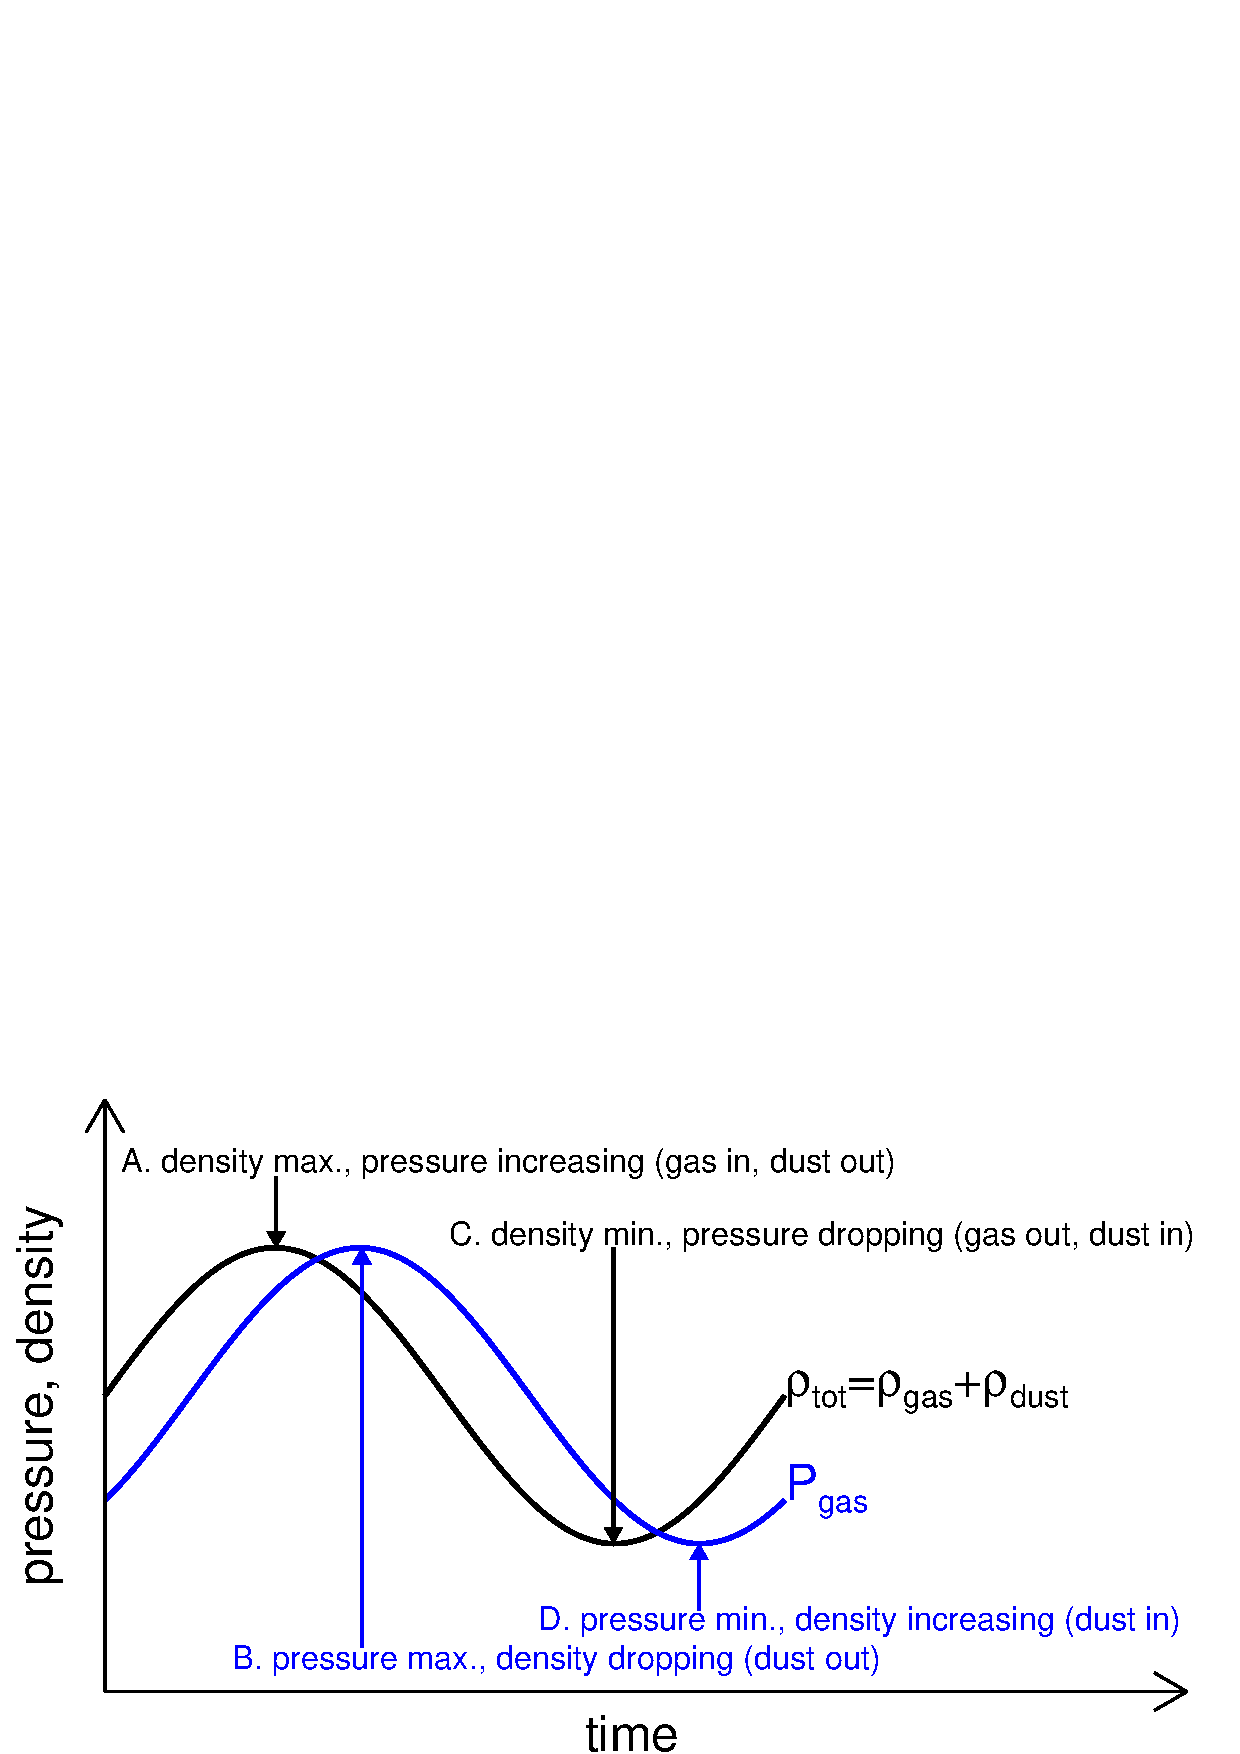
\includegraphics[width=\linewidth]{figures/drag}\\
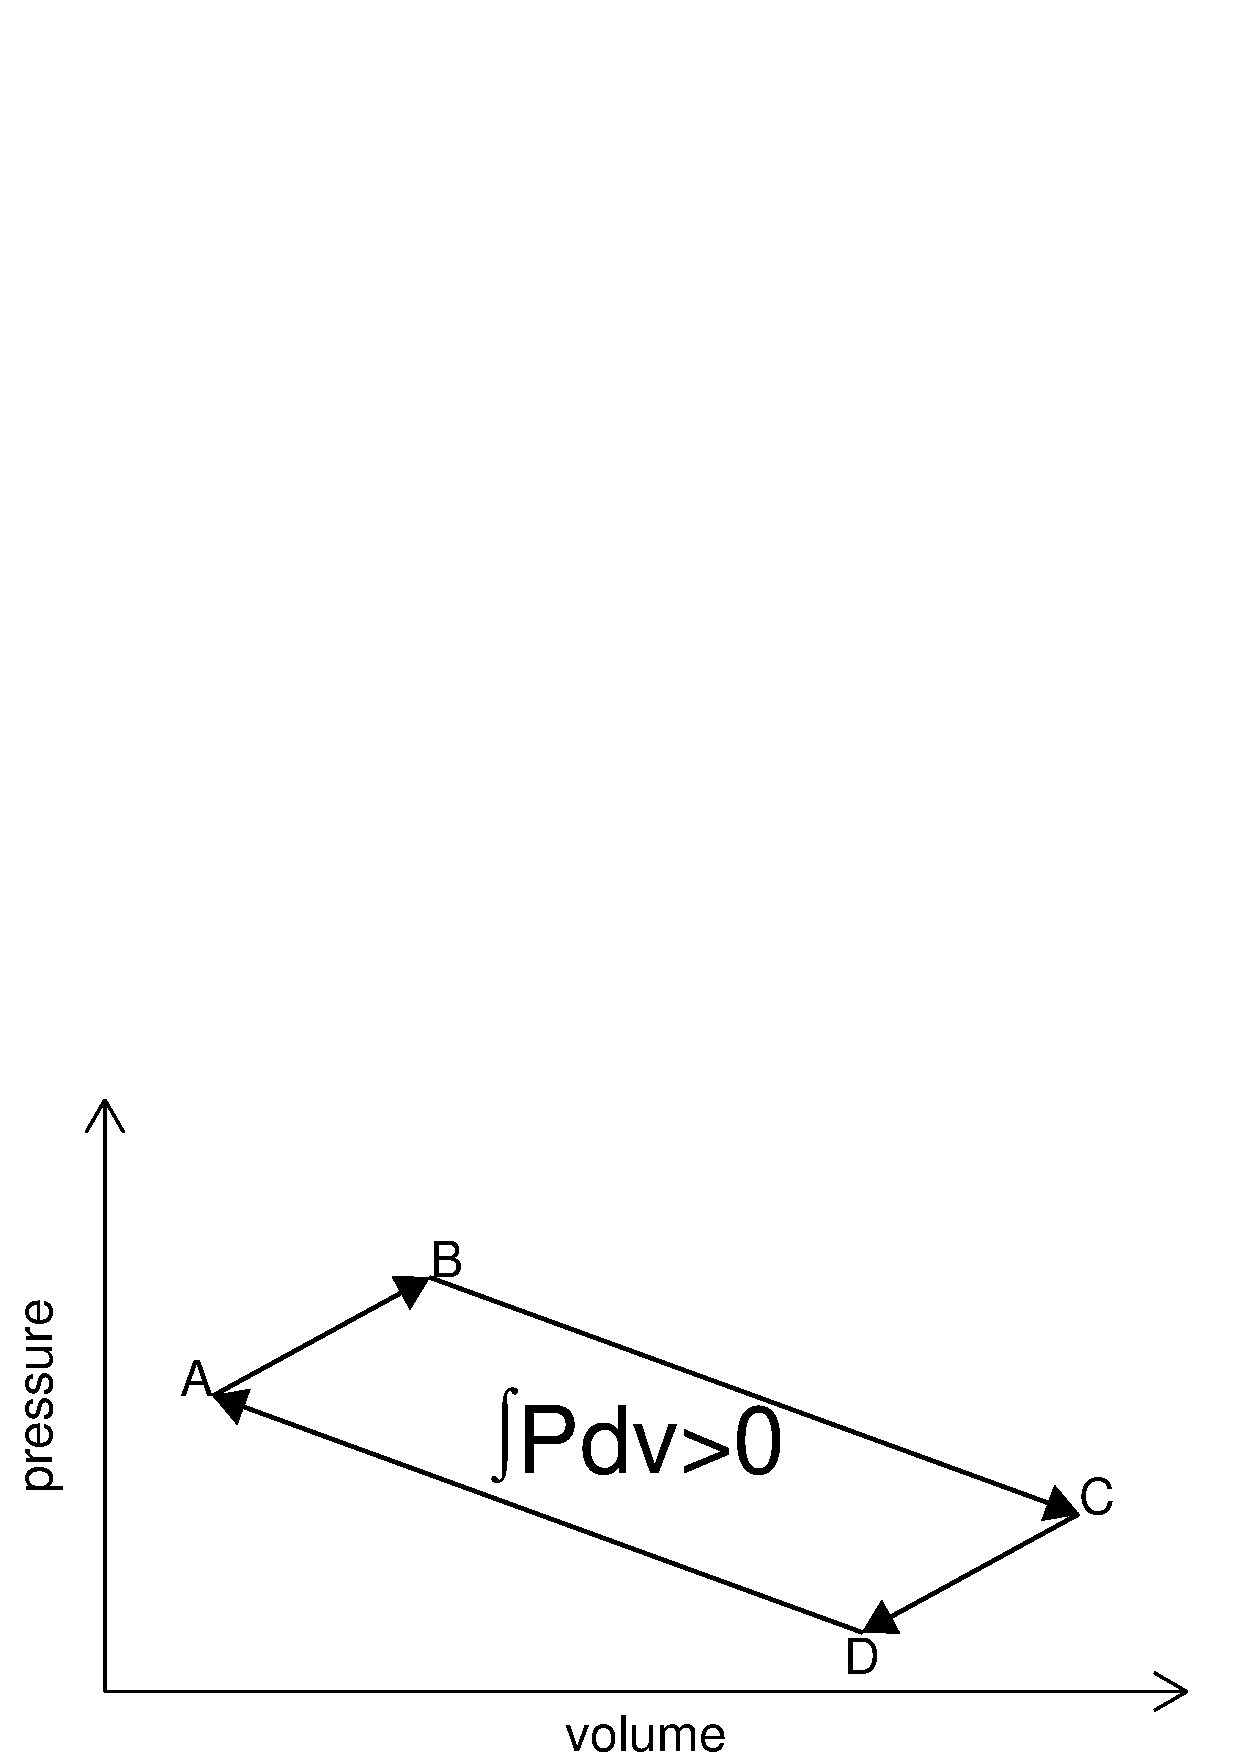
\includegraphics[width=\linewidth]{figures/pdv}
  \caption{Thermodynamic interpretation of overstable modes caused by
    dust-gas drag. Top: pressure and density evolution in time. 
    Bottom: oscillation cycle in the P-V plane. In the case shown,
    dust-drag causes 
    pressure to lag behind density, which results in a clockwise path in
    the P-V plane, implying positive work done by the fluid and
    hence would lead to growing oscillation amplitudes.  
    \label{pdv_cartoon}
  }
\end{figure}

This thermodynamic interpretation does not explain 
\emph{why} drag forces causes gas pressure to lag behind the dust
density, but merely shows 
that this \emph{must} be the case for any growing modes associated the
dust-gas drag. To rigorously understand how dust-drag causes this 
lag requires an explicit solution to the linearized equations with 
detailed treatment of the function $\mathcal{C}$. However, given the complexity of
$\mathcal{C}$ (see Appendix \ref{lin_dust}), we might generally expect
the dusty disks to  support a range of stable and unstable modes, with the
latter being associated with pressure-density lag. 

Indeed, \cite{jacquet11} explains the essence of the streaming 
instability in dusty protoplanetary disks as dust accumulation
(and hence compression) at a pressure bump, which then drags the 
gas towards it (and hence heating) to strengthen the pressure
bump. That is, heating occurs upon compression, as in stellar  
pulsational instabilities \citep{cox67}. In \S\ref{si} we check that the
streaming instability fits into this thermodynamic interpretation in
the strong drag limit.  

%A phase difference was also noted in the 
%numerical calculations of the streaming instability by 
%\citet{youdin07b}.    

%Whether the phase
%difference is positive or negative depends on the cooling function
%$\mathcal{C}$, but we may expect a system to generally have both
%modes, and that with a phase lag are unstable. 

\subsection{Locally isothermal gas perfectly coupled to dust}\label{dusty_vsi_int}
If $c_s(r,z)$ is non-uniform but $\tstop=0$, Eq. \ref{int_rel} 
gives  
\begin{align}
%  s = \frac{\imag\int P
%  \left(\nabla\cdot\dd\bm{v}^*\right)\left(\dd\bm{v}\cdot\nabla\ln{c_s^2}\right)dV}{2\omega\int\rho\left(|\dd 
%    v_r|^2 + |\dd v_z|^2\right)dV}. \label{vsi_check} 
  s = \frac{\imag\int P
    \left(\nabla\cdot\dd\bm{v}^*\right)\left(\dd\bm{v}\cdot\nabla\ln{c_s^2}\right)dV}{2\omega\mathcal{I}^2}. \label{vsi_check} 
\end{align} 
This is VSI caused by vertical shear arising from a radial
temperature gradient \citep{nelson13,barker15,lin15}. We present 
numerical solutions of the VSI with perfectly-coupled dust in \S\ref{results}. 

\section{Linear problem for perfectly coupled dust}\label{linear_problem}
We calculate explicit solutions to the linearized
equations in the limit of perfectly coupled dust ($\tstop=0$), so that
the equilibria defined in \S\ref{eqm} are exact steady states. We 
consider radially-localized axisymmetric disturbances of the form  
\begin{align}
  \delta f (r, z) = \delta f_1(r,z)\exp{(\ii k r)},
\end{align} 
%and similarly for $\dd P$ and $\dd\bm{v}$. 
where $k$ is a real wavenumber such that $|kr|\gg 1$, and the
amplitude $\dd f_1(r,z)$ is 
a slowly-varying function of $r$. Then 
$\p_r\to i k$ when acting on the above primitive perturbations, and we may
neglect curvature terms. We take  
$k>0$ without loss of generality. Hereafter, we drop the subscript 1
on the amplitudes. 
%The frequency $\sigma = \omega +
%\ii s$ is generally complex, with $\omega$ being the real frequency
%and $s$ is the real growth rate. 

Introducing 
\begin{align}
  W \equiv \frac{\dd\rho}{\rho}, \quad Q \equiv \frac{\dd P}{\rho},
\end{align}
the linearized equations for 
locally isothermal, perfectly-coupled dusty gas with the pressure
equation in place of the dust-fraction
(Eq. \ref{masseq}---\ref{momeq}, Eq. \ref{eff_energy}) are then:    

\begin{align}
  \ii\sigma W &= \ii k \dd v_r + \dd v_z^\prime +
  \dd v_r \p_r\ln{\rho} + \dd v_z\p_z\ln{\rho},\label{lin_mass}\\
  -\ii\sigma\dd v_r  &= 2\Omega\dd v_\phi + 
  \delta\bm{F}\cdot\hat{\bm{r}},\label{lin_xmom}\\
  \ii\sigma\dd v_\phi &= \frac{\kappa^2}{2\Omega}\dd v_r + \frac{\p
    v_\phi}{\p z}\dd v_z, \label{lin_ymom}\\
  -\ii\sigma\dd v_z &=  \delta\bm{F}\cdot\hat{\bm{z}},\label{lin_zmom}\\
  \ii\sigma Q &= \frac{P}{\rho}\left(\ii k \dd v_r + \dd
               v_z^\prime\right) + \frac{1}{\rho}\left(\dd v_r\p_rP + \dd v_z \p_zP\right)\notag\\
                &\phantom{=}-\frac{P}{\rho} \dd v_r\p_r
               \ln{c_s^2}, \label{lin_energy} 
%+ \dd v_z \p_z\ln{c_s^2}\right),\label{lin_energy} 
%               - \frac{\dd\mathcal{C}}{\rho},\label{lin_energy} 
\end{align}  
where $^\prime \equiv \p_z$ and $\dd\bm{F}$ is the linearized pressure
force, given in Appendix \ref{lin_press}. Note that we have assumed a
temperature profile that only depends on $r$.  

%; and 
%\begin{align}
%  \delta \bm{F} \equiv \frac{\dd\rho}{\rho^2}\nabla P -
%  \frac{1}{\rho}\nabla\dd P, 
%\end{align}
%$\dd\mathcal{C}$ is the linearized dust-duffusion function, given in
%Appendix \ref{lin_dust}. We consider stopping times appropriate for
%small grains in the Epstein regime. Note that for the axisymmetric
%problem, $\dd\bm{F}$ is purely meridional. 

Eq. \ref{lin_mass}---\ref{lin_energy} is a set of ordinary
differntial equations in $z$. All coefficients and amplitudes are
evaluated at a fiducial radius $r=r_0$, but their full $z$-dependence
is retained.  Two boundary conditions are needed for the $\tstop=0$
problem. This is expected since this problem is exactly equivalent to
 adiabatic hydrodynamics \citep[e.g.][]{lubow93}. For simplicity
we impose solid boundaries so that $\delta v_z(\pm\zmax)=0$. 

We solve the linearized equations as a generalized eigenvalue problem 
using a pseudo-spectral code adapted from \cite{lin15}. Amplitudes 
are expanded in Chebyshev polynomials up to order $N_z=512$. We check
results using Eq. \ref{vsi_check}.    

%\subsection{Boundary conditions}



























%Eq. \ref{lin_mass}---\ref{lin_energy} can be reduced to a set of
%first-order differential equations for $W, Q$ and $\dd v_z$. We can
%see this schematically as follows. Eq. \ref{lin_xmom} and
%\ref{lin_ymom} may be combined to yield 
%\begin{align*}
%  \dd v_r = \dd v_r (W, Q, \dd v_z). 
%\end{align*} 
%We can then take the continuity equation as an equation for $\dd v_z$, 
%\begin{align*}
%\text{Eq. \ref{lin_mass}} \Rightarrow \dd v_z^\prime(z) = \dd
%  v_z^\prime(W,Q,\dd v_z),
%\end{align*}
%and the vertical momentum equation as an equation for $Q$, 
%\begin{align*}
%\text{Eq. \ref{lin_zmom}} \Rightarrow Q^\prime(z) = 
% Q^\prime(W,Q,\dd v_z). 
%\end{align*}

%Now, for finite dust-gas coupling, $\tstop\neq0$, inspection of $\dd C$
%(Appendix \ref{lin_dust}) shows that it involves $W^\prime$ (assuming
%$\tepsilon < 1$). Then Eq. \ref{lin_energy} may be taken as a
%differential equation for $W$. However, for perfectly coupled dust,
%$\tstop =\dd\mathcal{C}= 0$. In that case Eq. \ref{lin_energy} gives an algebraic
%relation between $W$, $Q$ and $\dd v_z$. That is,
%\begin{align*}
%\text{Eq. \ref{lin_energy}}\Rightarrow \begin{cases}
%  W^\prime(z) = W^\prime(W, Q, \dd v_z) & \text{if } \tstop \neq 0, \\
%  W           (z) = W(Q, \dd v_z) & \text{if }\tstop = 0.
%\end{cases}
%\end{align*} 

%This means that for the perfectly coupled problem, we have a pair of
%ODEs for $Q$ and $\dd v_z$, and 
%When
%$\tstop\neq0$, we require three boundary conditions. {\bf WHAT?? Why odd
%  number of BCs? Shouldn't we have even number of BCs? We have
%two boundaries? I've only seen problems like this involving even
%number of BCs.} In this case we impose $\dd v_z =0$ at $z=\pm
%z_\mathrm{max}$, and classify modes according to their symmetry about
%the midplane: `even' modes with $\dd v_z^\prime(0) = 0$, and `odd' 
%modes with $\dd v_z(0)=0$.       


\section{
  Vertical shear instability with dust}\label{results} 

We now present numerical solutions for vertically stratified,
non-self-gravitating disks, assuming perfectly coupled dust. 
We formally take $\tstop=0$ so the equilibrium defined in \S\ref{eqm} 
are exact steady states. In reality,   
%\subsection{Validity}
%{\bf maybe incorporate into intro to this section?}
%We considered $\tstop=0$ in order to perform stability analysis on an
%exact steady state. 
%When $\tstop\neq0$, a stratified dusty 
%disk initialized as in \S\ref{eqm} would evolve 
%as 
dust settles to the midplane on a timescale $t_\mathrm{settle}\sim 
1/\tstop\OmK^2$ \citep{takeuchi02}. However, we expect the 
perfectly-coupled limit to be valid  
provided timescales of interest $t_\mathrm{grow}\ll
t_\mathrm{settle}$. For the VSI this translates to 
%Since VSI growth rates are $O(h_\mathrm{g}\OmK)$, 
%we require  
%\begin{align}
 $ \tstop\OmK \ll h_\mathrm{g}. $
%\end{align} 
For thin PPDs, this is satisfied for $\tstop\OmK \ll O(10^{-2})$.   


We first consider constant
midplane dust-to-gas ratios $\epsilon_0$ and characteristic thickness
$H_\epsilon$. Then the dust-to-gas ratio $\epsilon=\epsilon(z)$. In 
this limit any growing modes must be associated with the imposed
temperature gradient (see \S\ref{limits}). We are then studying the
effect of dust-loading on the VSI previously studied in pure gas
disks \citep[][\citetalias{lin15} in this section]{lin15}. In 
\S\ref{varHd} we allow $\p_r\epsilon\neq 0$, and in 
\S\ref{vert_mixed} we consider VSI driven entirely by radial
gradients in the dust-to-gas ratio (as discussed in
\S\ref{iso_perfect}).  

The parameters for the linear problem includes $\epsilon_0$, the dust
layer thickness $\Hd$, and the perturbation radial wavenumber
$k_x$. We choose a midplane gas density profile 
$\rho_\mathrm{g0}\propto r^{-3/2}$. The fiducial power-law 
index for the temperature profile is $q=-1$; and we set the gas disk
aspect-ratio $h_\mathrm{g}=0.05$. These values were also used by  
\citetalias{lin15}. 

%Two boundary conditions are needed for the $\tstop=0$
%problem \citep[e.g.][]{lubow93}. 
We impose solid vertical boundaries so that $\delta
v_z(\pm\zmax)=0$. We solve the linearized equations as a generalized
eigenvalue problem using a pseudo-spectral code adapted  
from \citetalias{lin15}. Amplitudes are expanded in Chebyshev
polynomials up to order $512$. %We check results using
%Eq. \ref{vsi_check}.      

\subsection{Qualitative expectations}\label{vsi_est}
\citetalias{lin15} found the appropriate way to compare 
vertical shear (destabilizing) and  vertical buoyancy (stabilizing)
is $r\p_z\Omega/\OmK$  against $N_z^2/\OmK^2$. From 
\S\ref{vertshear} and \S\ref{vbuoyancy} we find $|r\p_z\Omega|\sim q
h_\mathrm{g}\OmK$ for a 
thin, gas dominated disk; while $N_z^2\sim \epsilon\OmK^2$. Thus we
expect dust-induced buoyancy forces to stabilize the disk against the
VSI where $\epsilon \gtrsim h_\mathrm{g}$. 

%\begin{align}

\subsection{Effect of dust-loading}
We first vary the midplane dust-to-gas ratio 
$\epsilon_0\in[10^{-3},1]$, fixing the dust thickness to  
$\Hd=0.99\Hg$. Then  $\epsilon$ is roughly constant with height. We
set the vertical domain to $\zmax=5\Hg$.  

Fig. \ref{compare_vshear_fixHd} compares the basic state
vertical shear rate, which is destabilizing, and the vertical buoyancy
frequency, which is stabilizing. For the nearly dust-free disk
$\epsilon_0=10^{-3}$ the vertical shear dominates buoyancy for all
$|z|>0$. However, a heavy dust-load with $\epsilon_0=1$ renders the 
buoyancy to dominate over vertical shear in the disk atmosphere 
$|z|\gtrsim 2.5\Hg$. We thus expect instability all heights for 
$\epsilon_0=10^{-3}$, but to be restricted to the midplane for
$\epsilon_0=1$. 

\begin{figure}
  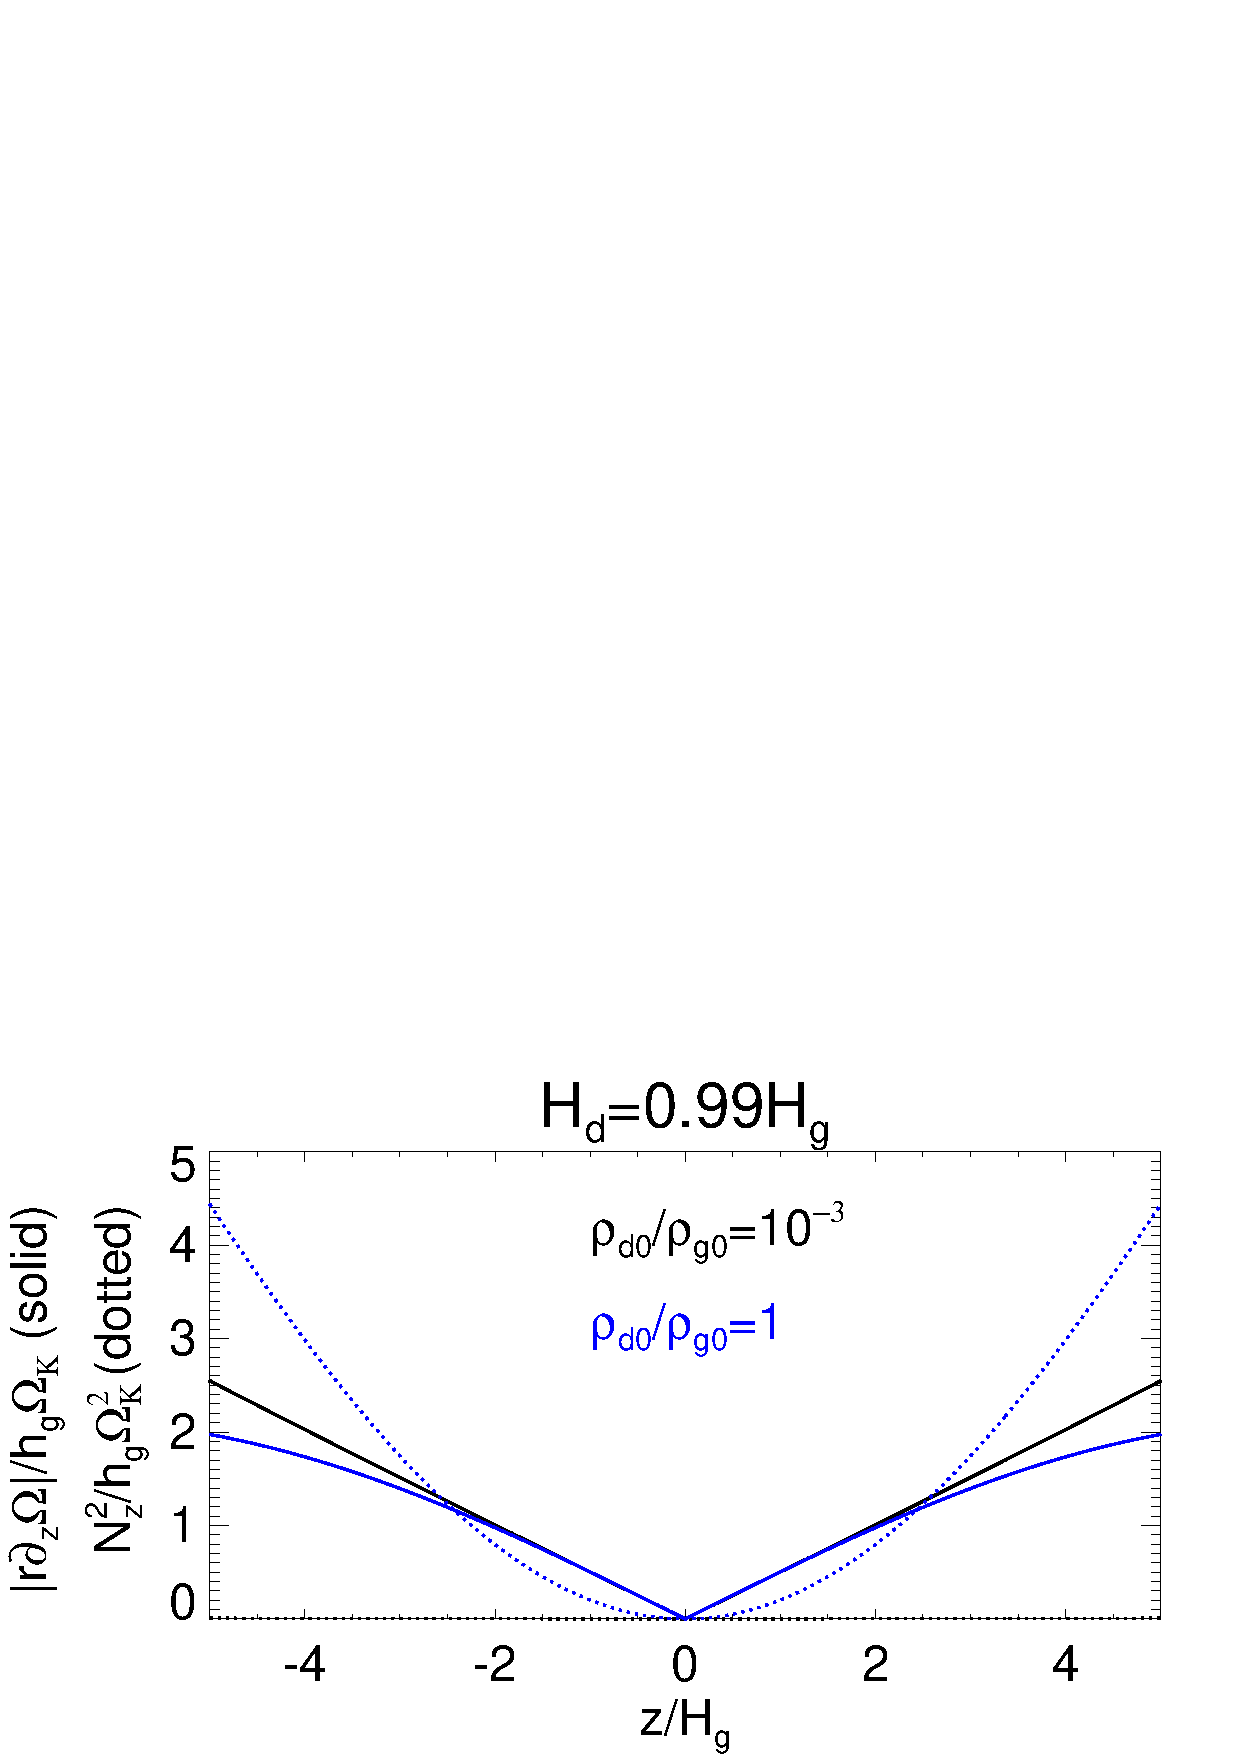
\includegraphics[width=\linewidth]{figures/compare_vshear_Nz2_fixHd} 
  \caption{Vertical shear rate (solid) compared to vertical buoyancy
    (dotted) in a locally isothermal, dusty disk with midplane dust-to-gas ratio
    of $\epsilon_0=10^{-3}$ (black) and $\epsilon_0=1$ (blue). 
    The dust layer thickness is fixed to $\Hd=0.99\Hg$ so the 
    dust-to-gas ratio $\epsilon$ is approximately constant with
    height. Vertical buoyancy here is due to dust-loading. 
    \label{compare_vshear_fixHd}
    }
\end{figure}

Fig. \ref{vsi_dust_loading} show unstable modes for different values
of $\epsilon_0$ with fixed perturbation wavenumber  $k_x\Hg = 30$. The
eigenvalue distributions for $\epsilon_0 \leq 10^{-2}$ are similar to the
dust-free fiducial case considered by \citetalias{lin15}. This is
expected since $\epsilon_0 < \hgas$ (\S\ref{vsi_est}). Eigenvalues 
consists 
of the roughly horizontal `body modes', and the nearly-vertical
`surface modes' \citep[which are associated with the imposed vertical
boundaries, ][]{barker15}.   

We find that increasing the dust-to-gas ratio reduce VSI growth
rates. Notably, surface modes, which are typically fastest growing in
the dust-free case, are suppressed in dusty disks for $\epsilon_0\geq
0.1$ (i.e. $\epsilon_0> \hgas$).   
The body modes' growth rates remain $ O(h_\mathrm{g}\OmK)$ 
but their oscillation frequency increases with
dust-loading, i.e. it increases with the vertical buoyancy. 
The total number of modes do not change 
significantly. This is in contrast with the effect of increasing
cooling times in an adiabatic gas disk, for which \citetalias{lin15}
find fewer unstable modes. 
%until the system is eventually completely stable. 

\begin{figure}
  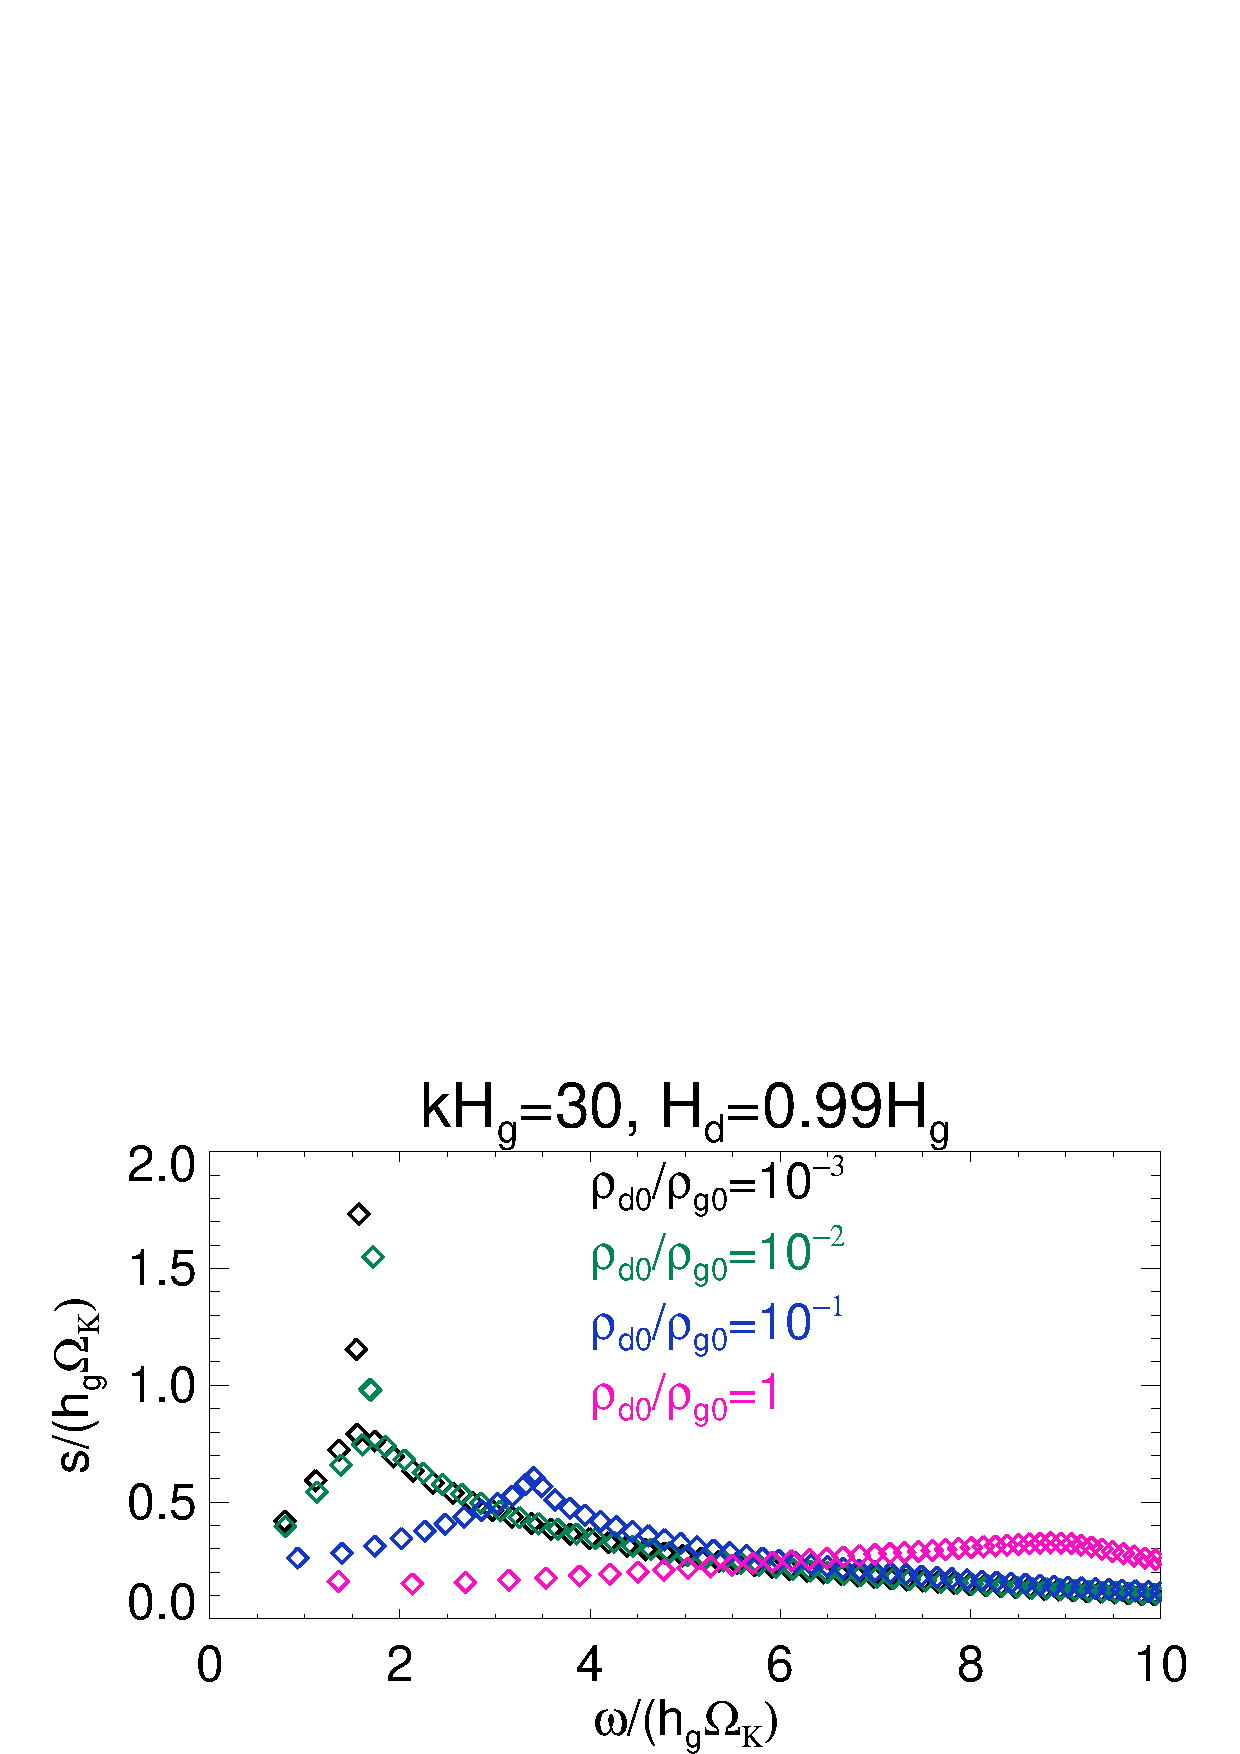
\includegraphics[width=\linewidth]{figures/compare_eigenvals_kx30Hd1} 
  \caption{Unstable modes in a locally isothermal, perfectly coupled
    dusty disk with fiducial parameters
    $(p,q,h_\mathrm{g}, \Hd/\Hg )=(-1.5,-1,0.05, 0.99)$. The real
    frequency $\omega$ and growth rates $s$ are shown for a range of
    midplane dust-to-gas ratios $\epsilon_0=\rho_\mathrm{g0}/\rho_\mathrm{d0}$. 
    \label{vsi_dust_loading}
    }
\end{figure}

The lowest frequency `fundamental' body mode is energetically dominant
because the entire disk column is perturbed \citep[cf. surface modes
  which only disturb the disk boundaries,][]{umurhan16c}. In Fig. \ref{vsi_dust_loading2d}
we compare the fundamental mode between the nearly 
dust-free case $\epsilon_0=10^{-3}$ an a dusty disk with
$\epsilon_0=1$. Dust-loading preferentially
stabilizes the disk atmosphere against the VSI, restricting
meridional motions to $|z|\lesssim 2\Hg$. 
This is consistent with Fig. \ref{compare_vshear_fixHd} comparing the basic state vertical
shear and buoyancy. % Notice also maxium perturbtions to the dust-to-gas ratio,
% $\delta\epsilon$, shifts from disk boundaries 
% to the midplane.  

\begin{figure}
%  \includegraphics[scale=0.54, clip=true, trim=0cm 2.5cm 0cm 0cm]{figures/result2d_dg1d-3.ps}\\
%  \includegraphics[scale=0.54]{figures/result2d_dg1.ps} 
\includegraphics[scale=0.32, clip=true, trim=0.5cm 0cm 3cm 0cm]{figures/result2d_dg1d-3.ps}\includegraphics[scale=0.32, clip=true, trim=1.8cm 0cm 0cm 0cm]{figures/result2d_dg1.ps}
  \caption{Fundamental dusty VSI mode in real space for midplane dust-to-gas
    ratio $\epsilon_0=10^{-3}$ (left) and $\epsilon_0=1$
    (right). The color scale shows the perturbation to the
    dust-to-gas ratio, $\delta\epsilon$; and the arrows show
    $\sqrt{\rho}\left(\dd v_x, \dd v_z\right)$. 
    \label{vsi_dust_loading2d}
    }
\end{figure}

In Fig. \ref{vsi_dust_loading_vareps} we plot the growth rates as a
function of $\epsilon_0$ for different perturbation wavenumbers
$k_x$. Dust-loading stabilizes the VSI more effectively for shorter
wavelength perturbations. This is because for high wavenumbers the
dominant modes are surface modes, which are effectively stabilized by
dust-loading as buoyancy forces are largest near the vertical 
boundaries. The figure suggest that VSI becomes much less efficient
for $\epsilon_0\gtrsim 0.1$ and $k_x\Hg\gtrsim 50$. 

\begin{figure}
  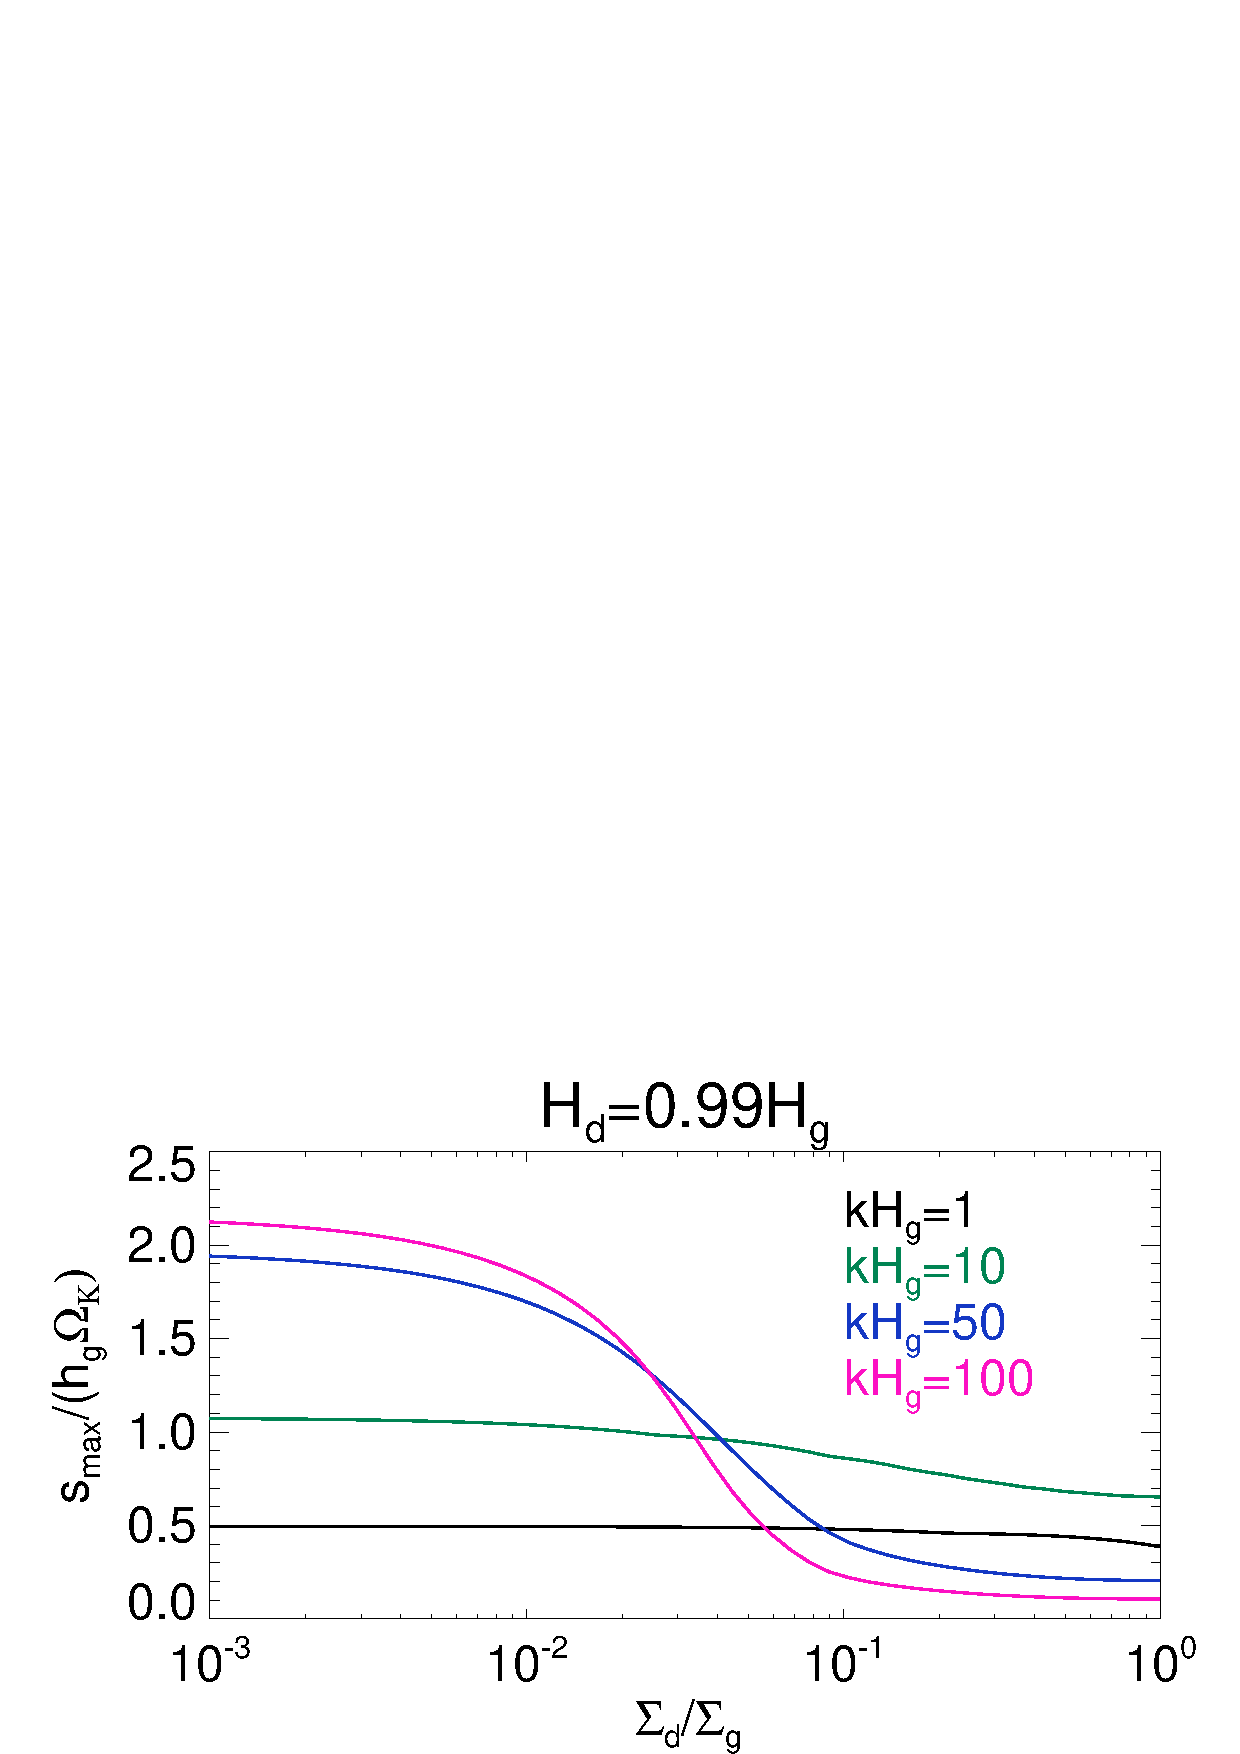
\includegraphics[width=\linewidth]{figures/compare_eigenvals_vareps2} 
  \caption{Maximum growth rate of the dusty VSI as a function of the
    midplane dust-to-gas ratio $\epsilon_0$ for perturbations with
    different radial wavenumbers $k$. The dust layer thickness is
    fixed to $\Hd\simeq \Hg$. 
    \label{vsi_dust_loading_vareps}
    }
\end{figure}




\subsection{Effect of dust layer thickness} 
We now vary $\Hd$ but fix the metalicity 
$Z \equiv \epsilon_0 \Hd/\Hg = 0.03$ to obtain $\epsilon_0$. Since we
will consider thin dust layers, here we use a smaller   
domain with $\zmax=2\Hg$ so that $\epsilon$ does not become
too small. 

We analyze two disks with $\Hd=0.1\Hg$ and 
$\Hd=0.99\Hg$. Fig. \ref{compare_vshear_fixZ} compares the vertical
shear  rate and buoyancy frequency. For $|z|\gtrsim 0.4\Hg$ the two
disks have the same profile with vertical shear dominating over
buoyancy. We thus expect perturbations away from the disk midplane in 
both cases. For $|z|\lesssim 0.4\Hg$, a thin dust 
layer with $\Hd=0.1\Hg$ boosts the vertical shear rate, but the
associated buoyancy is larger still, implying the mid-plane should be
stable. 
%Thus we expect the mid-plane of 
%the disk with $\Hd=0.1\Hg$ to have limited vertical motions.  

\begin{figure}
  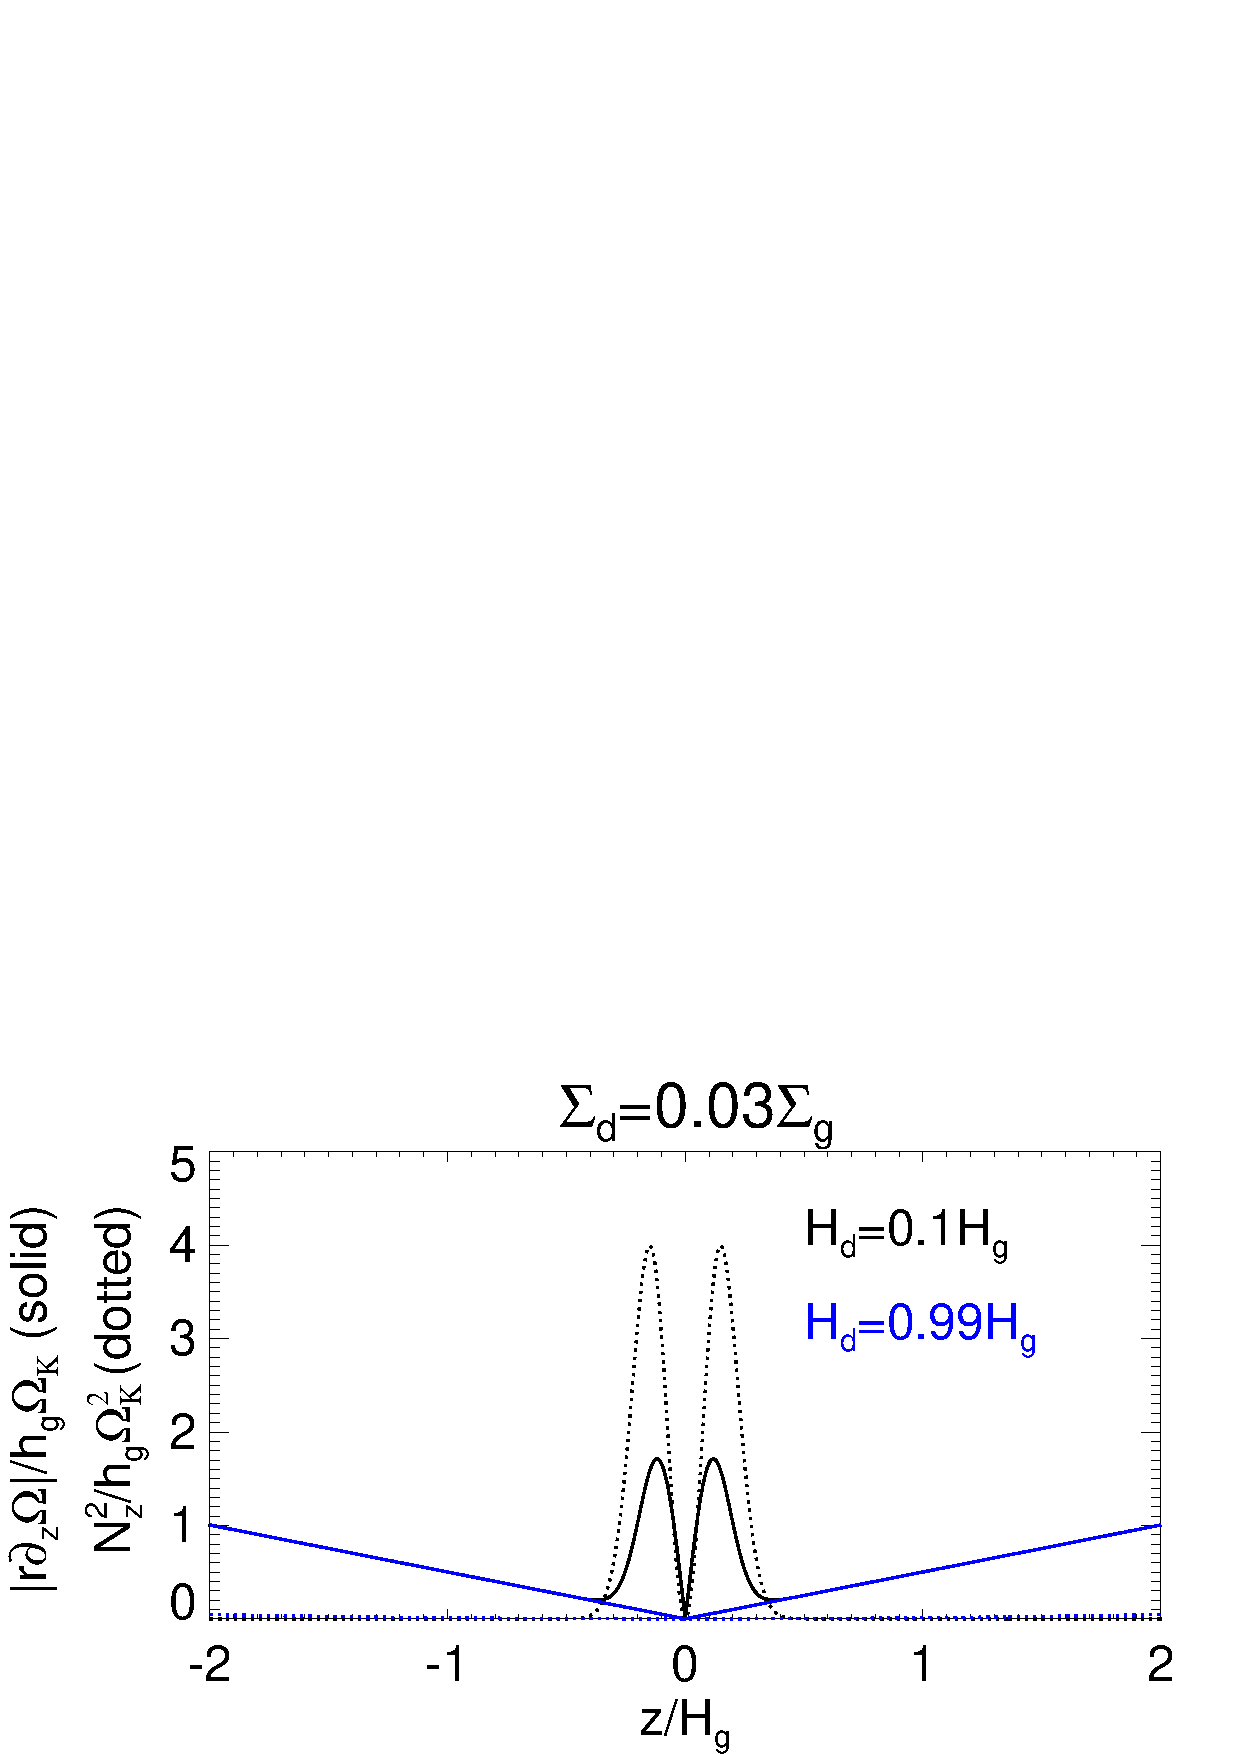
\includegraphics[width=\linewidth]{figures/compare_vshear_Nz2_fixZ} 
  \caption{Vertical shear rate (solid) compared to vertical buoyancy
    (dotted) in a locally isothermal, dusty disk 
    with metalicity $Z=0.03$ and dust thickness $\Hd=0.1\Hg$
    (black) and $\Hd=0.99\Hg$ (blue). 
    \label{compare_vshear_fixZ}
    }
\end{figure}

Fig. \ref{result2d_fixZ} compares the fastest growing VSI body modes  
with $k_x\Hg=30$ for the two cases above.\citepalias[The thinner domain
  adopted here eliminates surface modes, ][]{lin15}.   
We find very similar mode 
frequencies 
\begin{align*}
  \sigma = \begin{cases}
    \left(0.3053\ii - 0.8142\right)h_\mathrm{g}\OmK & \Hd=0.99\Hg, \\
    \left(0.3178\ii - 1.2237\right)h_\mathrm{g}\OmK & \Hd=0.1\Hg,
  \end{cases}
\end{align*}
since the vertical shear profile is similar throughout most of the
disk. However, meridional motions are suppressed near the midplane of
the $\Hd=0.1\Hg$ disk, as expected from the larger buoyancy frequency
relative to vertical shear there. This leads to a structure
analogous to PPD dead zones: a quiescent midplane between active
surface layers \citep{gammie96}.  


\begin{figure}
  \includegraphics[scale=0.32, clip=true, trim=0.5cm 0cm 3cm 0cm]{figures/result2d_Hd1.ps}\includegraphics[scale=0.32, clip=true, trim=1.8cm 0cm 0cm 0cm]{figures/result2d_Hd0d1.ps} 
  \caption{Fastest-growing dusty VSI mode in real space for midplane
    dust layer thickness $\Hd=0.99\Hg$ (left) and $\Hd=0.1\Hg$
    (right). The dust content is fixed to
    $\Sigma_\mathrm{d}=0.03\Sigma_\mathrm{g}$. 
    The color scale shows the perturbation to the
    dust-to-gas ratio, $\delta\epsilon$; and the arrows show
    $\sqrt{\rho}\left(\dd v_x, \dd v_z\right)$.
    \label{result2d_fixZ}
    }
\end{figure}

Fig. \ref{compare_eigenvals_fixZ} shows the maximum VSI growth rates
as a function of $\Hd$. As before, we find growth
rates are most affected by the vertical structure of the dust layer
when the perturbation wavenumer is large. Notice VSI growth rates converge as
$\Hd\to 0$. %to dust free values?    
Thus a thin dust layer, however large its associated vertical shear,
does not affect VSI growth rates. The non-monotonic behavior for $\Hd\gtrsim
0.5\Hg$ arises because the vertical buoyancy frequency 
\begin{align*}
N_z^2(H_d;z,Z) \simeq &Z\Hg z^2
\exp{\left(-\frac{z^2}{2\Hg^2}\right)}\OmK^2\notag\\
&\times 
\frac{1}{\Hd}\left(\frac{1}{\Hd^2} -
\frac{1}{\Hg^2}\right)\exp{\left(-\frac{z^2}{2\Hd^2}\right)}  
\end{align*}
is a non-monotonic function of $\Hd$ at fixed $z$. At $z=\Hg$ and $z=2\Hg$
the buoyancy frequency is maximized for $\Hd\simeq0.5\Hg$ and
$\Hd\simeq 0.8\Hg$, respectively. This is consistent with the abscissa
of minima in growth rates in Fig. \ref{compare_eigenvals_fixZ}. 

\begin{figure}
  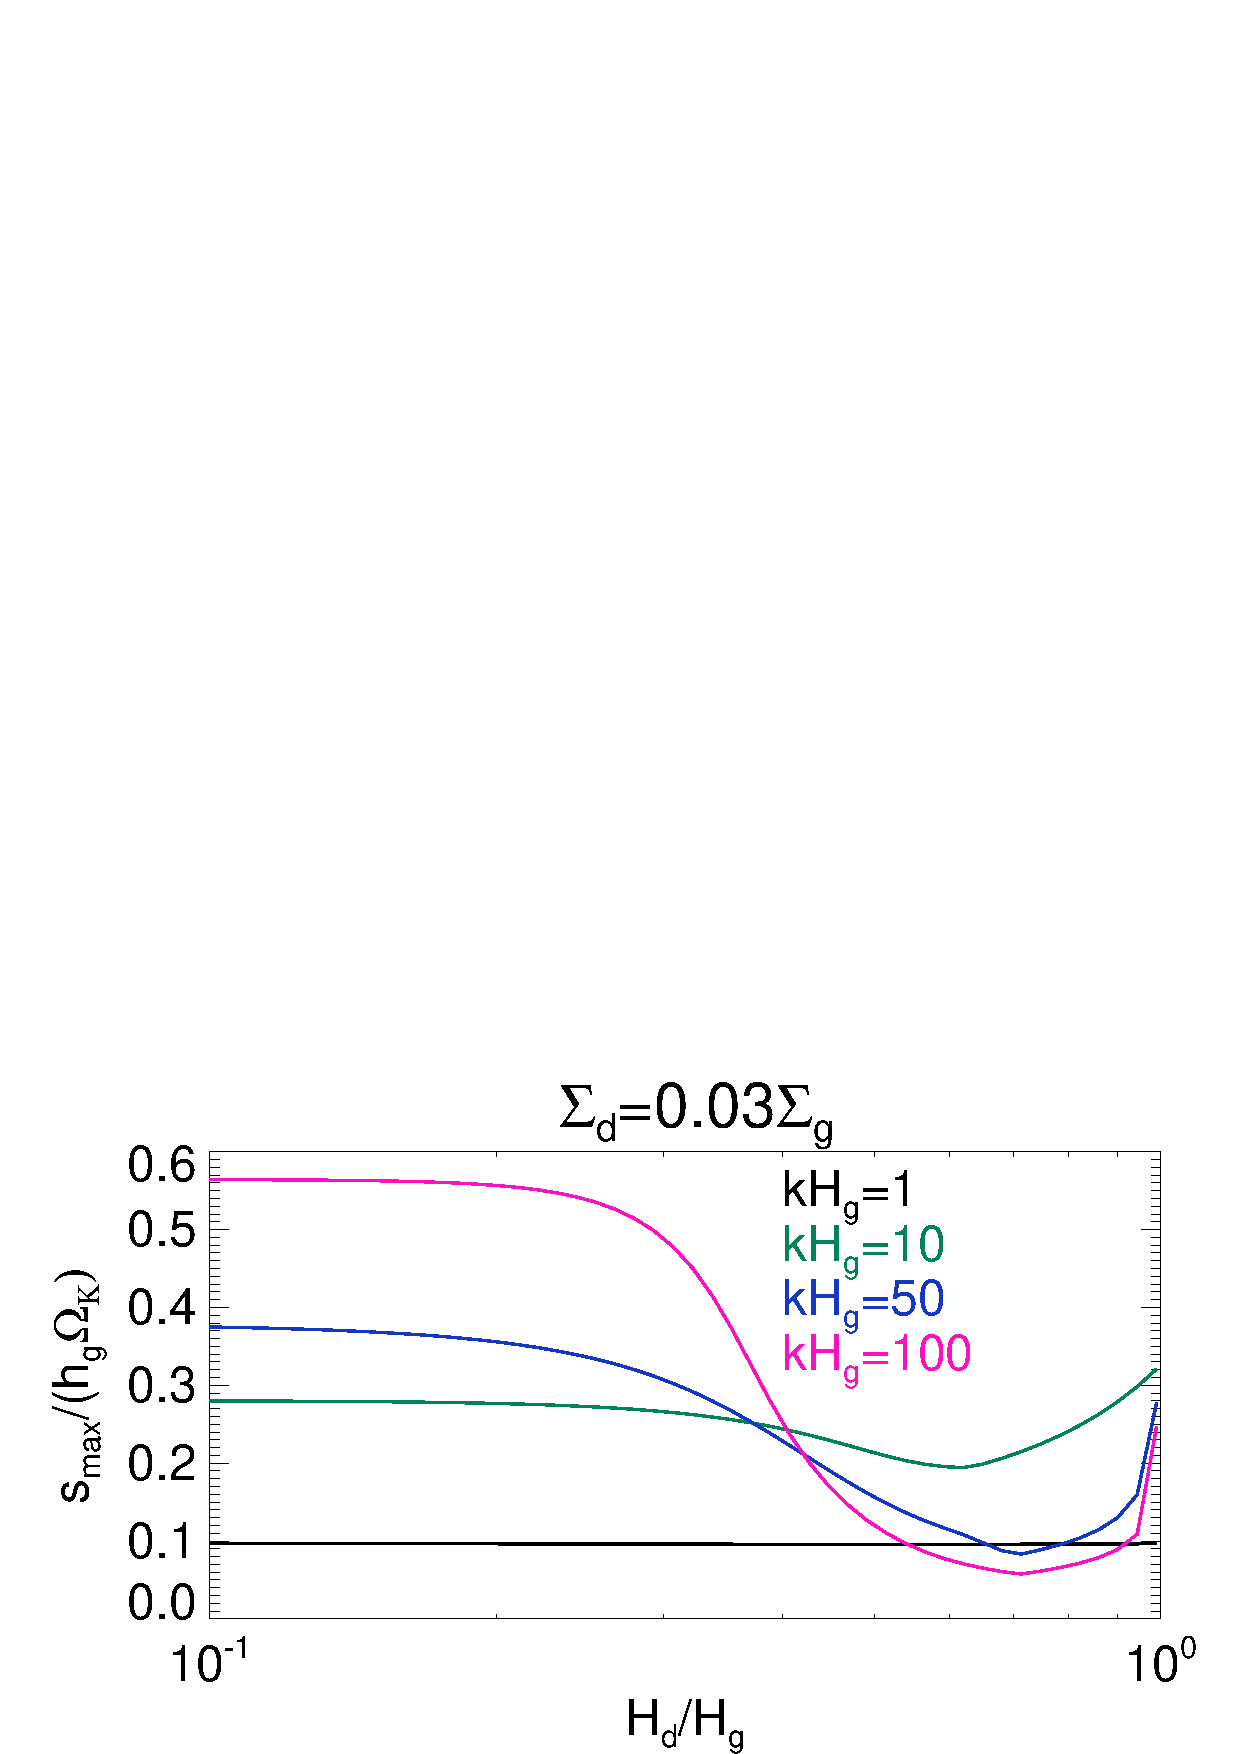
\includegraphics[width=\linewidth]{figures/compare_eigenvals_fixZ} 
  \caption{Maximum VSI growth rate for different perturbation
    wavenumbers $k$ as a function of the dust layer
    thickness $\Hd$ at fixed metalicity $Z=0.03$. 
    \label{compare_eigenvals_fixZ}
    }
\end{figure}

\subsection{Axisymmetric stability of ultra-thin dust layers}
The discussion in \S\ref{iso_perfect} imply strictly  
isothermal disks with a radially uniform dust-to-gas ratio are
stable against axisymmetric perturbations, no matter how thin the dust
layer is. We now demonstrate this numerically. 

To connect with similar studies, here  we also use 
the Richardson number $\rich \equiv N_z^2/\left(r\p_z\Omega\right)^2$
to label calculations \citep{youdin02}.   
Numerical simulations show    
non-axisymmetric instabilities develops when $\rich\lesssim0.1$, brought about
by very thin dust layers \citep{chiang08, lee10}. We show that \emph{axisymmetric}
instabilities never develop in radially uniform disks, however small $\rich$. 

We shall consider ultra thin dust layers with $\Hd\leq 0.01\Hg$ and thus
restrict the vertical domain to $\zmax = 0.02\Hg$. We fix the 
metalicity $Z=0.01$ so the midpane dust-to-gas ratio $\epsilon_0$ is 
$O(1)$.  We consider radial wavenumbers with $k_x\Hd=1$. 

Fig. \ref{ultra_thin} shows the maximum growth rate  as a function of
the radial temperature gradient, $q$. For all cases the vertical
shear is dominated by that due to the dust layer (see
\S\ref{vertshear}). However, we see that $s\propto
|q|$, i.e growth rates vanish in the strictly isothermal limit.  
In particular, this holds for $\rich < 0.1$, the critical value 
for non-axisymmetric instabilities. 

Axisymmetric instability here is associated with the thermal
contribution to vertical shear: as $q\to0$,  $\p_z\Omega$ becomes
entirely due to $\p_z\epsilon$ and there is no instability ($s\to
0$). This result is independent of $\rich$, so the Richardson number
is does not characterize the axisymmetric stability of dust
layers. 

\begin{figure}
  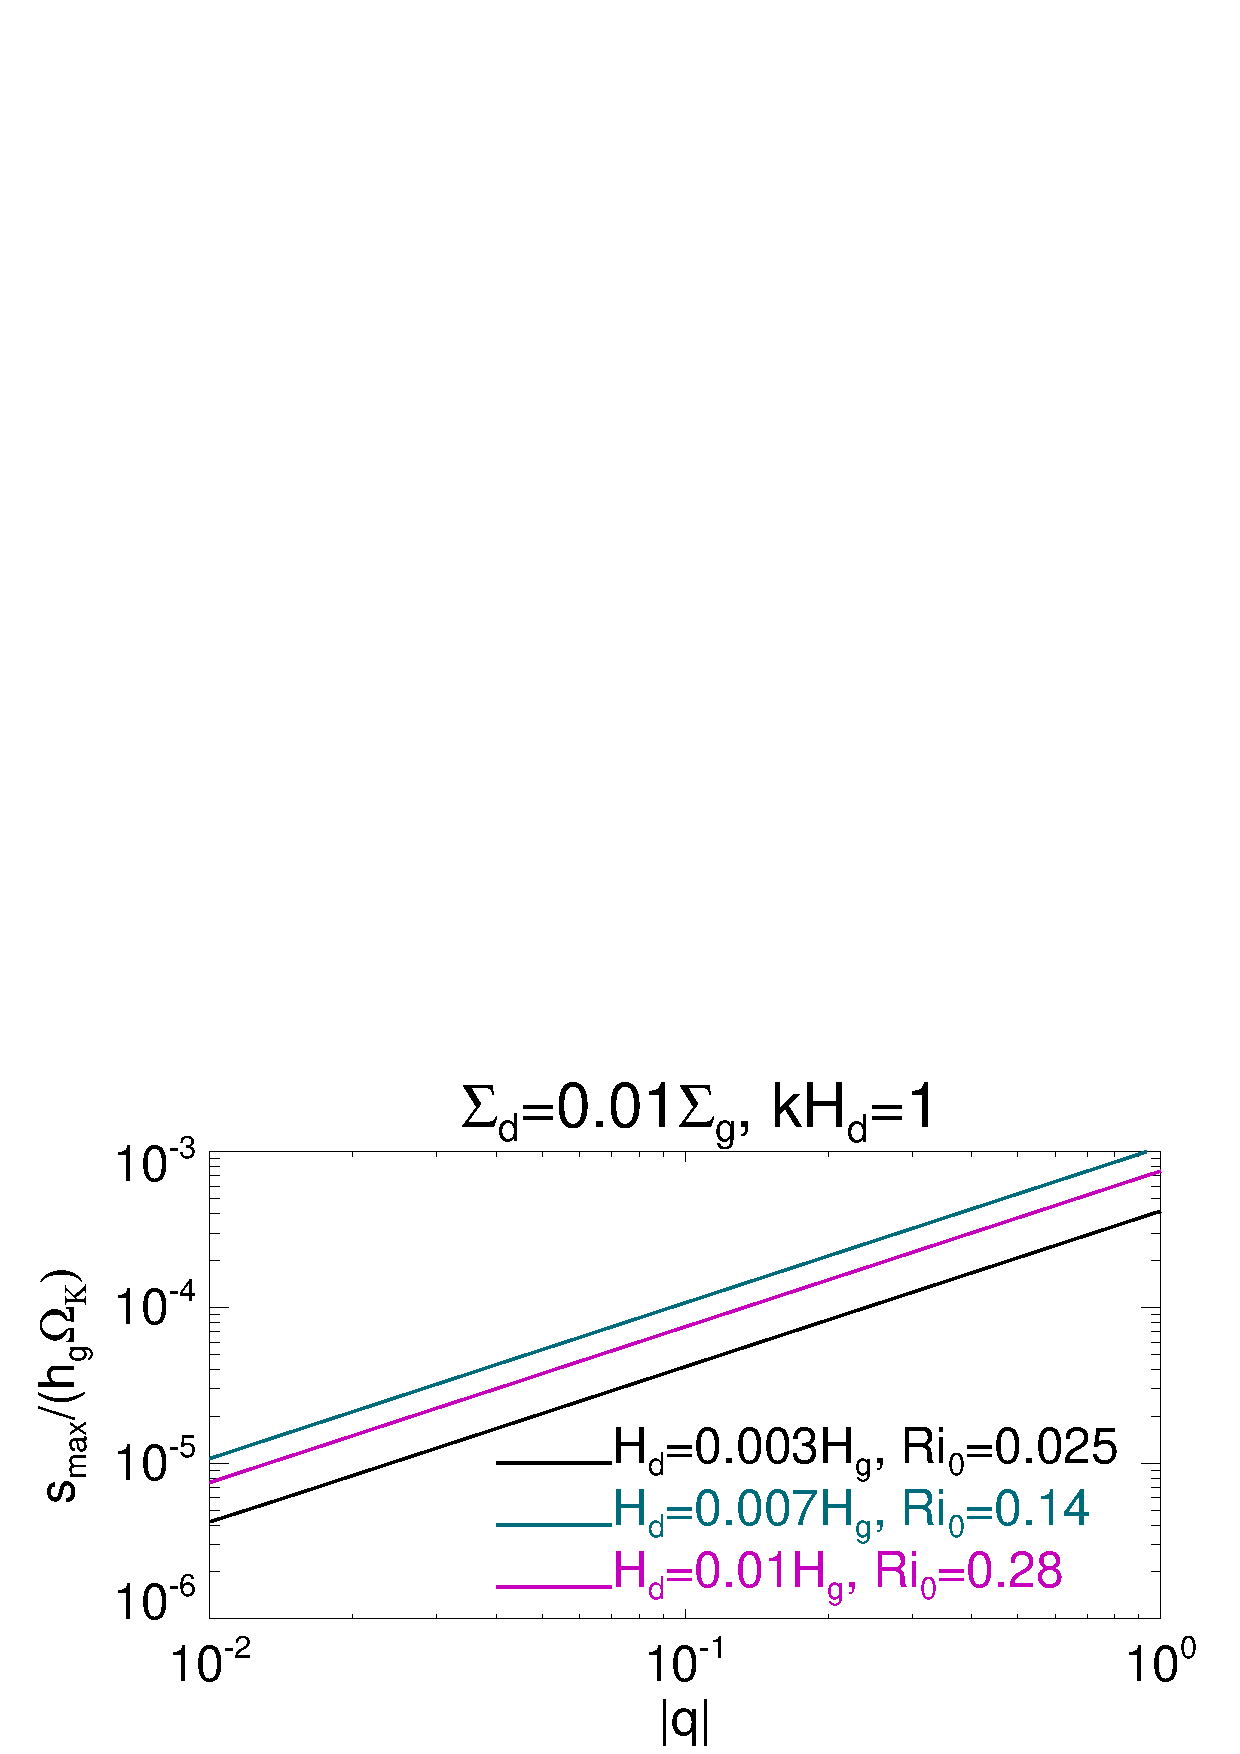
\includegraphics[width=\linewidth]{figures/compare_eigenvals_thindust} 
  \caption{Maximum VSI growth rate for ultra-thin dust layers $\Hd 
    \leq 0.01\Hg$ (with radially uniform dust-to-gas  ratio). Vertical shear is dominated by that due to 
    vertical dust stratification, but axisymmetric instability is still 
    associated with the radial temperature gradient $q$. 
 Here, $\rich_0$ is the minimum 
    Richardson number in the domain in the limit $q\to0$. The disk is stable to axisymmetric perturbations 
    in the strictly isothermal limit, regardless of the dust layer thickness. 
    \label{ultra_thin}
    }
\end{figure}




\subsection{Effect of a radially-varying dust-to-gas ratio}\label{varHd}
%{\bf bonus stuff, maybe delete in final version}

We now consider a radially-varying dust-to-gas ratio. Specifically we
let $\epsilon_0\propto r^{-1}$ and $H_\epsilon \propto \Hg$
(cf. constant values in the previous calculations). Then
\begin{align*} 
  \frac{\p\epsilon}{\p r} =
  \left(\frac{z^2}{H_\epsilon^2}\frac{d\ln{\Hg}}{dr} -
    \frac{1}{r}\right)\epsilon.   
\end{align*}
Here we fix $Z=0.01$, $\Hd=0.8\Hg$.       

Fig. \ref{compare_vshear_varHd} shows that a radially-varying
dust-to-gas ratio increases the magnitude of the vertical shear rate
away from the midplane (see also Eq. \ref{vshear2}). Thus we {
  typically} find higher VSI growth rates, as shown in
Fig. \ref{vsi_dust_varHd}. 
Surfaces modes, { appearing at high $k_x$}, are more effectively
enhanced by the additional vertical shear induced by
$\p_r\epsilon$. { Low frequency body modes with small
  $k_x$ are more affected by radial variations in the 
  dust-to-gas ratio than high-$k_x$, high-frequency body modes. }    

However, all growth rates remain
$O(\hgas\OmK)$. Importantly, the increase in the growth rate of the
fundamental mode is small. We do not expect the radial
dependence in $\epsilon$ to significantly affect the VSI in a dusty
disk. 

\begin{figure}
  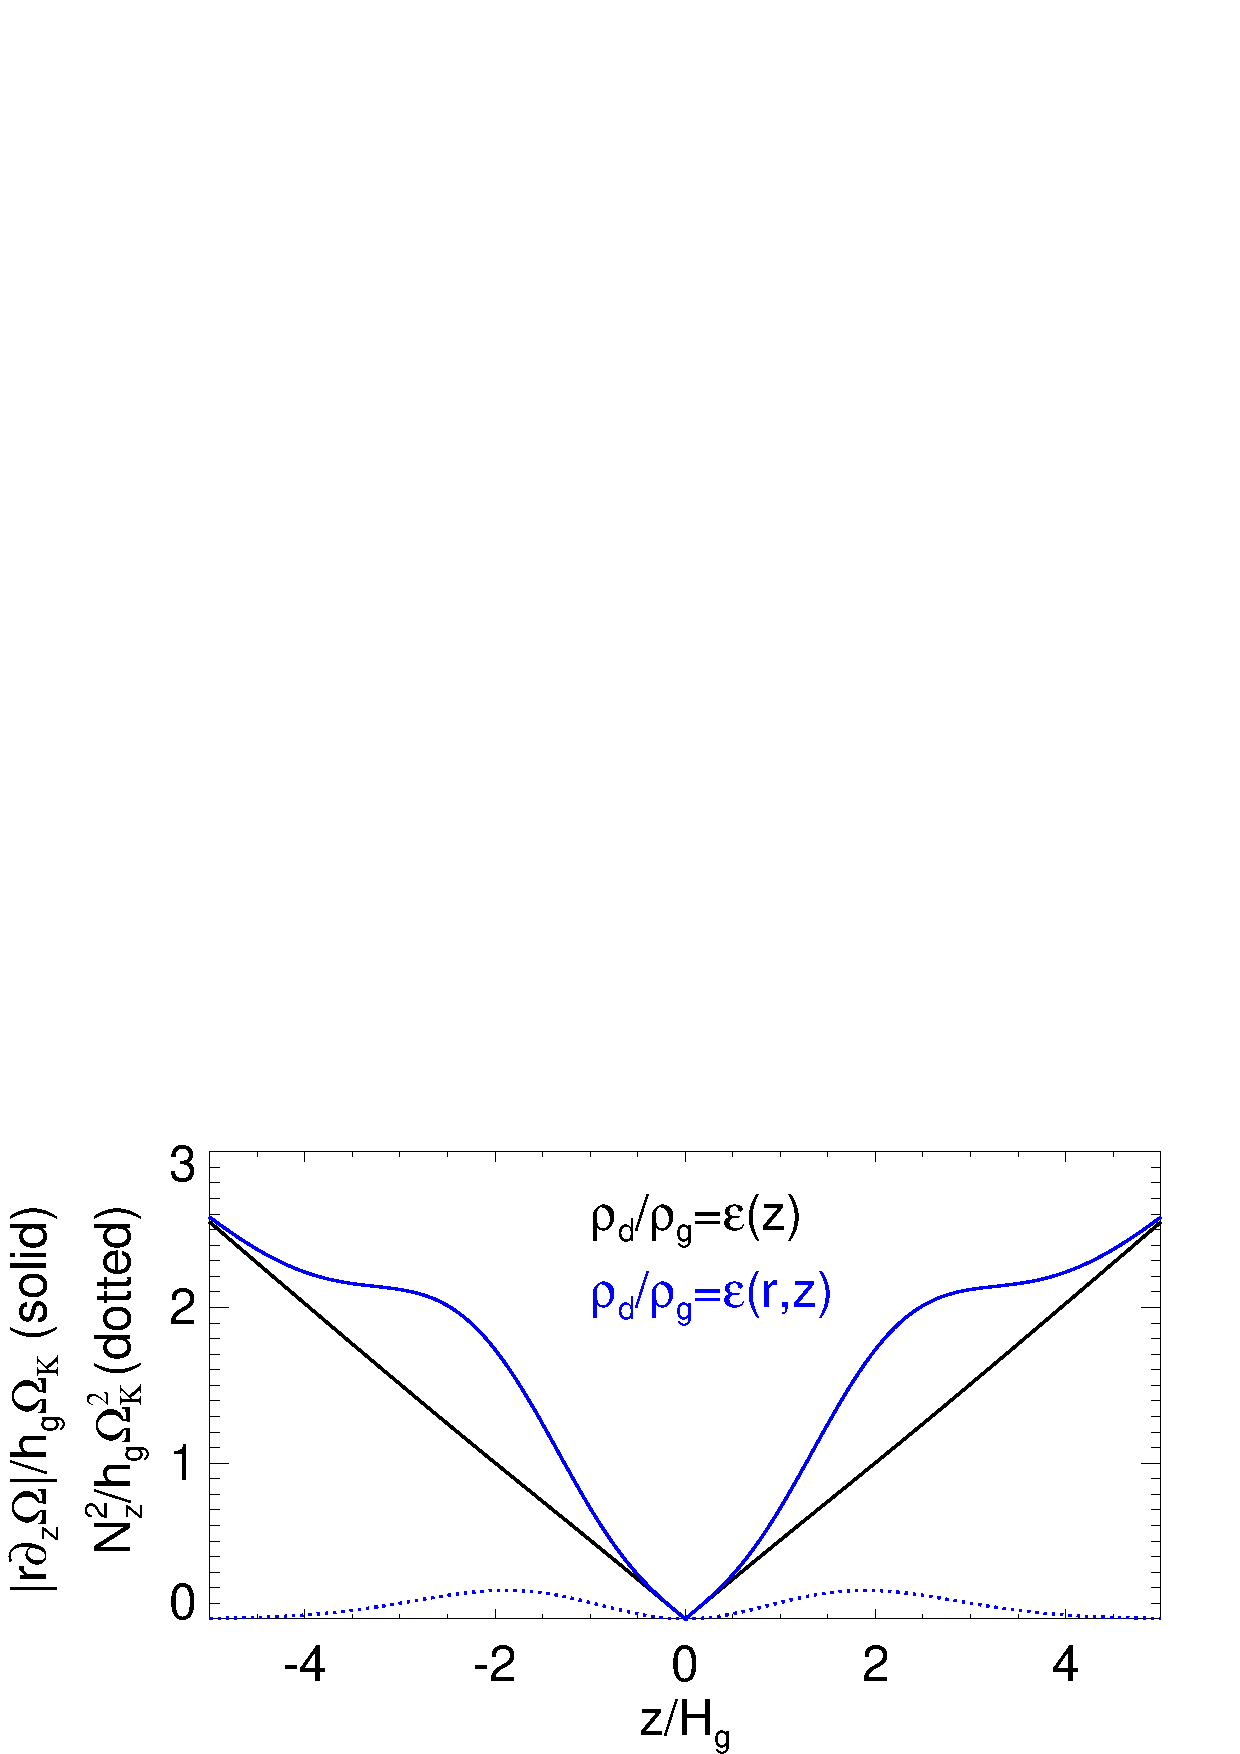
\includegraphics[width=\linewidth]{figures/compare_vshear_Nz2_varHd} 
  \caption{Vertical shear rate (solid) compared to vertical buoyancy
    (dotted) in a locally isothermal, dusty disk 
    with metalicity $Z=0.01$ and dust thickness $\Hd=0.8\Hg$.
    Black curves assume a dust-to-gas ratio that only depends on
    height; whereas the blue curve also allows a radial dependence in
    $\epsilon$. See text for details.  
    \label{compare_vshear_varHd}
    }
\end{figure}



\begin{figure}
  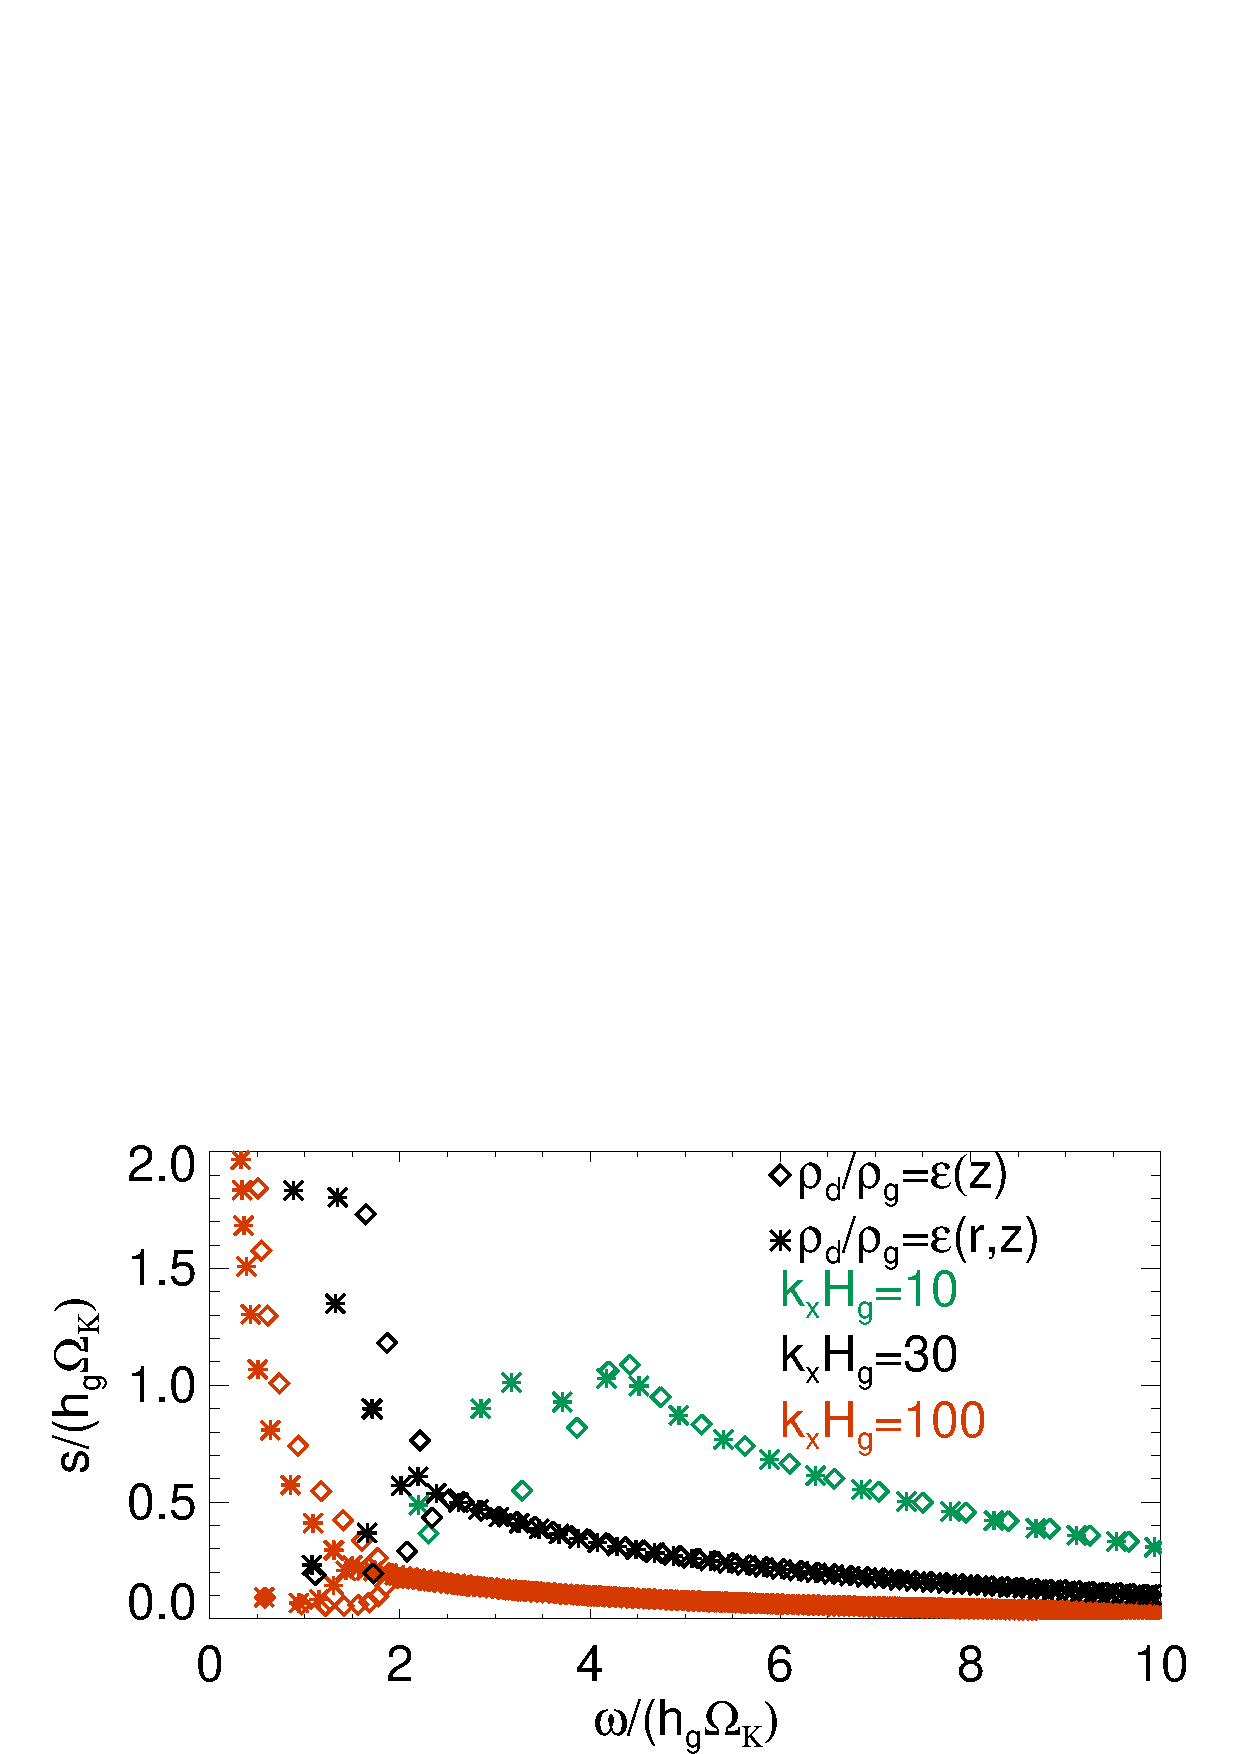
\includegraphics[width=\linewidth]{figures/compare_eigenvals_varHd} 
  \caption{Unstable VSI modes in the disk models of
    Fig. \protect\ref{compare_vshear_varHd}. { Diamonds (asterisks) 
    are mode frequencies for a disk with radially uniform (varying)
    dust-to-gas ratio. The radial wavenumbers are $k_xH_g = 10$
    (green),$k_xH_g = 30$ (black) and $k_xH_g = 100$ (orange). }
    \label{vsi_dust_varHd}
    }
\end{figure}

\subsection{Pure instability with vertically well-mixed
  dust}\label{vert_mixed} 

In \S\ref{iso_perfect} we found that for strictly isothermal
disks, a vertically-uniform dust-to-gas ratio can be unstable
if $d\epsilon/dr\neq0$.   
{
To demonstrate this numerically we set $q=0$ and $H_\mathrm{d}$ such
that $H_\epsilon=10^3\Hg$. We let $\rhod/\rhog \propto r^{-d}$
with different power indices $d$. The metalicity is fixed to $Z=0.03$.  
In these cases vertical shear $\p_z\Omega$ is 
attributed to the radially-varying dust-to-gas ratio (see
Eq. \ref{vshear2}).    
}

{ We show unstable modes in 
Fig. \ref{vert_mixed_modes}.} 
%In order to obtain appreciable growth   
%rates, we consider super-Solar metalicity $Z=0.03$ and high
%radial wavenumber $k_x\Hg=1800$. 
As expected from the discussion in
\S\ref{iso_perfect}, the disk admits purely growing modes with
$\omega=0$. This is distinct from the growing oscillations associated
with classic VSI discussed above. 

{ We find in smooth disks large 
  $k_x$ is needed for appreciable growth rates, e.g. $k_xH_g=1800$
  with $\rhod/\rhog\propto r^{-1}$. 
  Local shearing box simulations may 
  be required to study the non-linear evolution of such short 
  wavelengths \citep[e.g.][]{bai10b,yang16}. Alternatively, as shown in Fig. \ref{vert_mixed_modes},
  a rapidly varying dust-to-gas ratio permits dynamical instability at
  longer radial wavelengths, which might be resolvable in global disk 
  simulations. 
}

\begin{figure}
  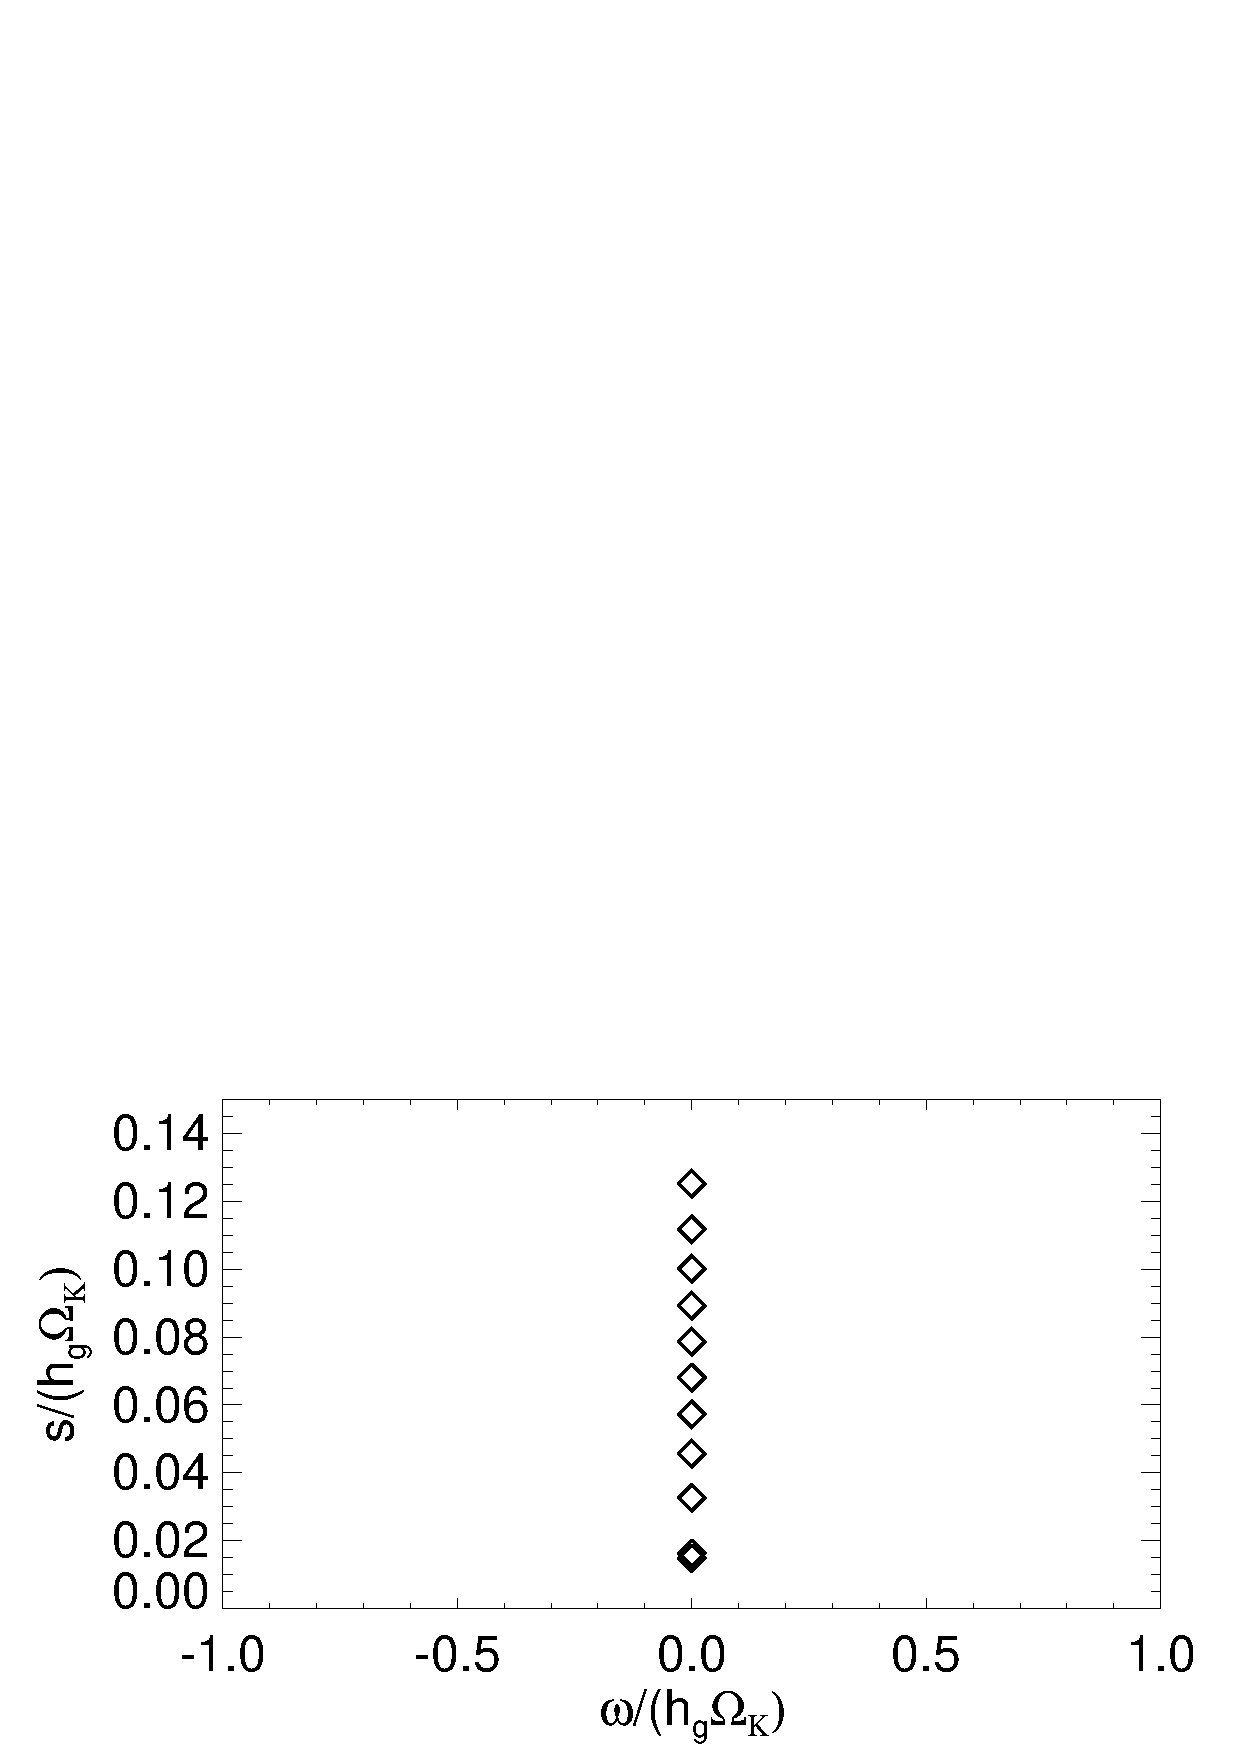
\includegraphics[width=\linewidth]{figures/vert_mixed_modes} 
  \caption{Purely growing modes in a strictly isothermal disk ($q=0$) with
    vertically uniform dust-to-gas ratio. The instability is due to 
    vertical shear $\p_z\Omega\neq0$ arising from radial variations in
    the dust-to-gas ratio, $d\epsilon/dr\neq 0$. \label{vert_mixed_modes}
    }
\end{figure}

%{\bf
%  \subsection{Implications for protoplanetary disks}
%dust settling, dust-induced buoyancy 
%The above calculations 
%radial d/g -> radial temp profile 
%}



\section{Summary and discussion}
In this paper we highlight the similarity between an isothermal 
dusty gas and an adiabatic, pure gas. 
In the limit of perfect dust-gas coupling, the dust content of a fluid 
parcel $\rhod/\rhog$ is conserved. This is analogous to entropy being 
conserved following a adiabatic, pure gas. %s = s(\rhod/\rhog)
We explicitly show that for 
a locally isothermal, dusty gas that the evolutionary equation of 
$\rhod/\rhog$ may be recast into an effective energy equation identical
in form to that in standard adiabatic hydrodynamics. We find the 
natural definition of the entropy of the dusty gas is 
\begin{align*}
  s  = \ln{\left(\frac{c_s^2\rhog}{\rhog+\rhod}\right)}.  
\end{align*}
This allows us to define the buoyancy frequency of an isothermal 
dusty gas. 

%
%finite coupling/heat source 

Finite dust-gas friction causes a relative drift between the two
components of the mixture. Then $\rhod/\rhog $ is no
longer conserved following a fluid parcel, as it is allowed to
exchange dust particles with neighboring parcels owing to a non-zero
stopping time $\tstop$. This is analogous to heat exchange between a 
pure gas parcel and its surroundings. Thus, finite dust-gas friction
may be interepreted as an energy/entropy source term for the dusty
gas.   

%
In this first study, we apply this equivalence principle to study the
axisymmetric stability of locally isothermal, protoplanetary disks
perfectly coupled to dust ($\tstop=0$). This is so that we may 
compute exact, steady equilibria for analyses. Furthermore,
in this limit the dusty problem is \emph{identical} to adiabatic, pure
gas dynamics. 

We obtain the Solberg-Hoiland criteria to assess
axisymmetric stability when the equation of state is strictly
isothermal. We show that {\bf dust-settling cannot lead to
  axisymmetric instability, however large the associated vertical
  shear} \citep[cf. \emph{non-axisymmetric} Kelvin-Helmholtz instabilities
  induced by  dust-settling, ][]{lee10}. We also show that
sharp edges in the dust-to-gas ratio cannot persist in protoplanetary
disks, as these imply a sharp entropy gradient and may thus destablize
the disk. 

%does not preclude non-axisymmetric instabilities. but if there is a
%global radial temp gradient, then vertical shear arising from
%it will always be comparable to dust-settling. but there is vsi with
%global rad temp grad 

For locally isothermal disks $c^2_s=c_s^2(r)$ we generalize the vertical
shear instability (VSI) to include dust. We find that dust-loading
generally has a stabilizing effect. In our disk models
dust-loading does not affect VSI growth rates significantly, but
meridional motions may be suppressed at heights where vertical 
buoyancy dominates over vertical shear. This confirms our 
identification of the entropy and buoyancy of an isothermal, dusty
gas.  

%growth rates not sig changed 
%v shear from thin dust layers are overwhelmed by 

\subsection{Generalization to locally polytropic disks}
We can extend the dusty/adiabatic gas correspondence to 
other fixed equations of state. As an example, consider the locally
polytropic disk 
\begin{align}
  P = K(r,z)\rhog^{\Gamma}, 
\end{align}
where $K$ is a prescribed function and $\Gamma$ is the constant
adiabatic index. Then eliminating $\tepsilon$ from the dust equation
\ref{dusteq} gives 
\begin{align}
  \frac{D P}{D t} = - \Gamma P\nabla\cdot\bm{v}  + P \bm{v}\cdot\nabla \ln{K}
  + \frac{\Gamma P}{\rhog}\nabla\cdot\left(\tepsilon\tstop\nabla
  P\right).
\end{align}
Thus the dusty gas behaves like a pure gas with adiabatic index
$\Gamma$. The entropy is given by 
\begin{align}
  s = \ln{\left[K(r,z)\left(1 - \tepsilon\right)^\Gamma\right]}.  
\end{align}
When $K$ is constant, the corresponding Solberg-Hoiland criteria for
axisymmetric stability may be obtained from that in standard adiabatic 
hydrodynamics \citep[e.g.][]{tassoul78} by
using this definition of entropy in
Eqs. \ref{dusty_solberg1}---\ref{dusty_solberg2}. 

\subsection{Dusty analogs of other gaseous instabilities}  




%gi
%rwi 





%\subsection{Implication for numerical simulations}


\subsection{Thermodynamic interpretation of dusty instabilities}


%\subsection{Caveats and future directions}
%gi 

\acknowledgements
We thank P. Loren-Aguilar for initial discussions that motivated this study. We also thank 
C. Baruteau, R. Dong, J. Fung, S. Inutsuka, W. Lyra, M. Pessah, and O. Umurhan 
for comments during the course of this project. This work is supported
by the Theoretical Institute for Advanced Research in Astrophysics  
(TIARA) based in Academia Sinica Institute of Astronomy and
Astrophysics (ASIAA), NASA Astrophysics Theory Program grant
NNX17AK59G, and  
the Steward Theory Fellowship at the University of Arizona.   



\appendix
\section{Variational principle}\label{var_prin}

Here we consider the more general equation of state for the gas with
$P = K \rhog^{\Gamma}$ where $K$ is a prescribed function of position
and $\Gamma$ is a constant. The effective energy equation is then
Eq. \ref{poly_energy}. We also include the self-gravitational
potential $\psi$ of the gas
plus dust mixture, which satisfies 
%\begin{align}
$  \nabla^2 \psi  = 4 \pi G \rho. $
%\end{align} 
The linearized equations for axisymmetric
disturbances are  

\begin{align}
  \ii\sigma\frac{\delta\rho}{\rho} &= \nabla\cdot\dd\bm{v} +
  \dd\bm{v}\cdot\nabla\ln{\rho},\label{lin_mass_full}\\
%  \ii\sigma\frac{\delta P}{P} &= \nabla\cdot\dd\bm{v} +
   \ii\sigma\frac{\delta P}{P} &= \Gamma \nabla\cdot\dd\bm{v} +
  \dd\bm{v}\cdot\nabla\ln{P} - \dd\bm{v}\cdot\nabla\ln{c_s^2} - \frac{\dd\mathcal{C}}{P}.\label{lin_energy_full}\\
  -\ii\sigma\dd v_r  &= 2\Omega\dd v_\phi + 
  \hat{\bm{r}} \cdot \delta\bm{F} -  \hat{\bm{r}} \cdot \nabla\dd\psi ,\\
  \ii\sigma\dd v_\phi &= \frac{\kappa^2}{2\Omega}\dd v_r + \frac{\p
    v_\phi}{\p z}\dd v_z,\\
  -\ii\sigma\dd v_z &=  \hat{\bm{z}} \cdot \delta\bm{F}  -  \hat{\bm{z}} \cdot \nabla\dd\psi, \\ 
\nabla^2 \delta\psi & = 4\pi G \dd\rho. 
\end{align}  
where the linearizd pressure force $\delta \bm{F}$ is given in
Appendix \ref{lin_press}. These equations do not assume the
radially-local approximation used in the main text. From the
linearized meridional momentum equations, we find  

\begin{align}
  \sigma^2\int\rho\left(|\dd v_r|^2 + |\dd v_z|^2\right)dV = \int\left( \rho
  \kappa^2 |\dd v_r|^2 + \rho r\frac{\p \Omega^2}{\p z} \dd v_z \dd
  v_r^*  + \ii\sigma \rho \dd \bm{F}\cdot\dd\bm{v}^*
  - \ii \sigma \rho \nabla\dd\psi\cdot  \dd\bm{v}^* 
  \right)dV,\label{meridional}
\end{align}
where the integral is taken over the volume of the fluid. Integrating
by parts and ignoring surface integrals, the last term is
\begin{align}
  \int \ii\sigma\rho \dd \bm{F}\cdot\dd\bm{v}^*dV &=\int\left( \ii\sigma \frac{\dd
    \rho}{\rho}\dd\bm{v}^*\cdot \nabla P - \ii\sigma \dd
  \bm{v}^*\cdot\nabla \dd P  \right)dV\notag\\
&= \int\left( \ii\sigma \frac{\dd
    \rho}{\rho}\dd\bm{v}^*\cdot\nabla P + \ii\sigma \dd
 P  \nabla\cdot \dd \bm{v}^*  \right)dV\notag\\
 & = \int\left[
%   \left(
%   \ii\sigma \frac{\dd P}{P} - \dd\bm{v}\cdot\nabla s + \dd
%   \bm{v} \cdot \nabla \ln{c_s^2} + \frac{\dd\mathcal{C}}{P}
%   \right)\dd\bm{v}^*\cdot\nabla P  
   \left(
   \ii\sigma \frac{\dd P}{\Gamma P} - \dd\bm{v}\cdot\nabla \seff + \frac{\dd
   \bm{v}}{\Gamma} \cdot \nabla \ln{K} +
   \frac{\dd\mathcal{C}}{\Gamma P} \right)\dd\bm{v}^*\cdot\nabla P
   + \ii\sigma \dd P  \nabla\cdot \dd \bm{v}^*
   \right]dV\notag\\
 & = \int\left[
%   \ii\sigma\frac{\dd P}{P}\nabla\cdot\left(P\dd\bm{v}^*\right) +
%   \left(\dd\bm{v}^*\cdot\nabla P\right) \left(\dd\bm{v} \cdot \nabla
%   \ln{c_s^2} + \frac{\dd\mathcal{C}}{P}   -  \dd\bm{v}\cdot\nabla s\right) 
%   \right]dV\notag\\
   \ii\sigma\frac{\dd P}{\Gamma P}\left(\dd\bm{v}^*\cdot\nabla P +
   \Gamma P\nabla\cdot\dd\bm{v}^*   \right)
   +\left(\dd\bm{v}^*\cdot\nabla P\right) \left( \frac{\dd\bm{v}}{\Gamma} \cdot \nabla
   \ln{K} + \frac{\dd\mathcal{C}}{\Gamma P}   -  \dd\bm{v}\cdot\nabla \seff\right) 
   \right]dV\notag\\
 & = \int\left\{
%   \left[\frac{1}{P}\nabla\cdot\left(P\dd\bm{v}\right) -
%   \dd\bm{v}\cdot\nabla\ln{c_s^2} - \frac{\dd\mathcal{C}}{P}  \right]\nabla\cdot\left(P\dd\bm{v}^*\right)
%   +\left(\dd\bm{v}^*\cdot\nabla P\right)\left(\dd\bm{v} \cdot \nabla
%   \ln{c_s^2} + \frac{\dd\mathcal{C}}{P}   -  \dd\bm{v}\cdot\nabla s \right)
%   \right\}dV \notag\\
 \left[
   \nabla\cdot\dd\bm{v} +
  \frac{\dd\bm{v}}{\Gamma}\cdot\nabla\ln{P} -
  \frac{\dd\bm{v}}{\Gamma}\cdot\nabla\ln{K} -
  \frac{\dd\mathcal{C}}{\Gamma P}. 
  \right]
 \left(\dd \bm{v}^*\cdot\nabla P +
 \Gamma P\nabla\cdot\dd\bm{v}^*   \right)\right. \notag\\
 &\phantom{=\int\left\{\right\}}\left. 
 + \left(\dd\bm{v}^*\cdot\nabla P\right)\left(\frac{\dd\bm{v}}{\Gamma} \cdot \nabla
 \ln{K}
 + \frac{\dd\mathcal{C}}{\Gamma P}   -  \dd\bm{v}\cdot\nabla \seff \right)
 \right\}dV \notag\\
 &=\int\left[
%     \frac{1}{P}\left|\nabla\cdot\left(P\dd\bm{v}\right)\right|^2 -
%     \left(\dd\bm{v}^*\cdot\nabla P\right)\left(\dd\bm{v}\cdot\nabla s
%     \right) -
%     P\left(\nabla\cdot\dd\bm{v}^*\right)\left(\dd\bm{v}\cdot\nabla\ln{c_s^2} + \frac{\dd\mathcal{C}}{P} \right)  
    \frac{1}{\Gamma P} \Bigl\lvert \dd \bm{v}\cdot\nabla P +
 \Gamma P\nabla\cdot\dd \bm{v}    \Bigr\rvert ^2 - 
     \left(\dd\bm{v}^*\cdot\nabla P\right)\left(\dd\bm{v}\cdot\nabla \seff
     \right) -
      P\left(\nabla\cdot\dd\bm{v}^*\right)\left(\dd\bm{v}\cdot\nabla\ln{K} + \frac{\dd\mathcal{C}}{P} \right) 
     \right]dV,
\end{align}
where  $\seff\equiv\ln{(P^{1/\Gamma}/\rho)}$. 
The self-gravitational part of Eq. \ref{meridional} is, again
nelgecting surface terms when integrating by parts, 
\begin{align}
-\int \ii\sigma \rho \nabla\dd\psi \cdot\dd  \bm{v}^* &= \int \ii\sigma
  \dd\psi \nabla\cdot\left(\rho\dd\bm{v}^*\right) dV
 = \int \left|\sigma\right|^2 \dd\psi \dd \rho^*dV 
  = -\frac{1}{4\pi G}\int   \left|\sigma\right|^2
   \left|\nabla\psi\right|^2 dV,  
\end{align}
where the linearized continuity and Poisson equations have been used. 

Hence,
\begin{align}\label{integral_ex}
  &\sigma^2\int\rho\left(|\dd v_r|^2 + |\dd v_z|^2\right)dV \notag\\
&=  \int\left\{
  \rho |\dd v_r|^2 \left(\kappa^2 - \frac{1}{\rho}\frac{\p P}{\p
    r}\frac{\p \seff}{\p r}\right)
  + \rho |\dd v_z|^2\left(-\frac{1}{\rho}\frac{\p P}{\p
    z}\frac{\p \seff}{\p z}\right)
   + \rho \dd v_z \dd v_r^*\left(r\frac{\p\Omega^2}{\p z} -
  \frac{1}{\rho}\frac{\p P}{\p
    r}\frac{\p \seff}{\p z}\right) 
  + \rho \dd v_z^*\dd v_r \left(-\frac{1}{\rho}\frac{\p P}{\p
    z}\frac{\p \seff}{\p r}\right)\right. \notag\\
&\phantom{==\int}\left.+
%  \frac{1}{P}\left|\nabla\cdot\left(P\dd\bm{v}\right)\right|^2
 \frac{1}{\Gamma P}\Bigl\lvert \dd\bm{v}\cdot\nabla P +
 \Gamma P\nabla\cdot\dd\bm{v}     \Bigr\rvert^2
 - \frac{1}{4\pi G}\left|\sigma\nabla\dd\psi\right|^2 
  \right\}dV 
%  P\left(\nabla\cdot\dd\bm{v}^*\right)\left(\dd\bm{v}\cdot\nabla\ln{c_s^2}\right)dV
-\int    P\left(\nabla\cdot\dd\bm{v}^*\right)\left(\dd\bm{v}\cdot\nabla\ln{K}\right)dV
  -\int \left(\nabla\cdot\dd\bm{v}^*\right)\dd\mathcal{C}dV.  
\end{align}
Note that the coefficient of $\delta v_z\delta v_r^*$ and $\delta
v_z^*\delta v_r$ are equal owing to the equilibrium state
(Eq. \ref{vshear}). The non-self-gravitating case with $\Gamma=1,\, K = c_s^2$ gives
Eq. \ref{int_rel}. Similar integral relations are given by 
\cite{kato78, kley93,latter06}.  

%If $c_s$ is constant then the second integral vanishes, $\sigma^2$
%is real, and the first integral leads to the usual Solberg-Hoiland
%criteria. However, for a stationary but non-uniform temperature
%profile, the second  

\section{Linearized pressure forces and its divergence}\label{lin_press}
%Define
%\begin{align}
 % \bm{F} \equiv - \frac{\nabla P}{\rho}. 
%\end{align}
The linearized form of the pressure force $\bm{F} = -\nabla P/\rho$ is  
\begin{align}
  \delta \bm{F} = - \frac{\dd\rho}{\rho}\bm{F} -
  \frac{1}{\rho}\nabla\dd P,
\end{align}
with divergence
\begin{align}
  \nabla\cdot\dd\bm{F} = -
  \nabla\left(\frac{\dd\rho}{\rho}\right)\cdot\bm{F} -
  \frac{\dd\rho}{\rho}\nabla\cdot\bm{F} +
  \nabla\ln{\rho}\cdot\frac{\nabla\dd P}{\rho} -
  \frac{1}{\rho}\nabla^2\dd P. 
\end{align}

%\subsection{Explicit expressions}

The explicit forms for $\dd\bm{F}$ and $\nabla\cdot\dd\bm{F}$, in the
radially-local approximation, are
\begin{align}
  &\dd F_r = - W F_r - \ii k_x Q,\\
  &\dd F_z = - W F_z - \left[Q^\prime + Q
    \left(\ln{\rho}\right)^\prime\right]  = - \ii\sigma \dd v_z, 
\end{align} 
where the last equality is the linearized
vertical momentum equation; and 
\begin{align}
  \nabla\cdot\dd\bm{F} &= F_r\left(\p_r\ln{\rho} - \ii k_x \right)W - F_z
  W^\prime - W \nabla\cdot\bm{F} + \ii k_x Q \p_r\ln{\rho} +
  \left(\ln{\rho}\right)^\prime\left[Q^\prime + Q
    \left(\ln{\rho}\right)^\prime\right] \notag\\
  & \phantom{=} + k_x^2 Q - \left\{Q^{\prime\prime} + 2
    Q^\prime\left(\ln{\rho}\right)^\prime
    + Q\left[\left(\ln{\rho}\right)^{\prime\prime}+\left(\ln{\rho}\right)^{\prime
      2}\right]\right\}\notag\\
    &= \left[\left(\p_r\ln{\rho}-\ii k_x\right)F_r - \nabla\cdot\bm{F} +
      F_z^\prime\right]W + \left(\ii k_x \p_r\ln{\rho} + k_x^2\right)Q  -
      \ii\sigma \dd v_z^\prime.
\end{align}




\section{Linearized dust diffusion}\label{lin_dust}
We consider small grains in the Epstein regime, with fixed internal
density and size, so that
\begin{align}
  \tstop  =  \frac{K}{\rho c_s}\label{epstein}
\end{align}
\citep{price15}, where $K$ is a constant. Then the dust diffusion
function becomes
\begin{align}
  \mathcal{C} \equiv c_s^2\nabla\cdot\left(\tepsilon\tstop\nabla
  P\right) = - K c_s^2 \nabla\cdot
  \left(\frac{\tepsilon}{c_s}\bm{F}\right) =
  -Kc_s \left(\bm{F}\cdot\nabla\tepsilon + \tepsilon \nabla\cdot\bm{F}
  - \frac{1}{2}\tepsilon\bm{F}\cdot\nabla\ln{c_s^2}\right).  
\end{align}
Linearizing,
\begin{align}
  - \frac{\dd\mathcal{C}}{Kc_s} = \bm{F}\cdot\nabla\dd\tepsilon +
  \dd\bm{F}\cdot\nabla\tepsilon + \dd\tepsilon\nabla\cdot\bm{F} +
  \tepsilon\nabla\cdot\dd\bm{F} -
  \frac{1}{2}\nabla\ln{c_s^2}\cdot\left(\bm{F}\dd\tepsilon + \tepsilon
  \dd\bm{F}\right). 
\end{align}
The linearized dust-fraction $\dd\tepsilon$ and its derivatives in the
radially-local approximation are given by
\begin{align}
  \dd\tepsilon      &= (1-\tepsilon)W - \frac{Q}{c_s^2}, \\
  \p_r\dd\tepsilon &= \left[(1-\tepsilon)\left(\ii k_x -
    \p_r\ln{\rho}\right) - \p_r\tepsilon\right]W + \left(\p_r\ln{c_s^2}
  + \p_r\ln{\rho} - \ii k_x \right)\frac{Q}{c_s^2},\\
  \dd\tepsilon^\prime &= (1-\tepsilon)W^\prime - \tepsilon^\prime W -
  \left(\frac{Q}{c_s^2}\right)^\prime. 
\end{align}

%\section{Conversion formulae}
%The gas density $\rhog$ and dust-to-gas ratio $\epsilon$ is related
%to the total density $\rho$ and dust-fraction $\tepsilon$ by
%\begin{align}
%  \ln{\rho} &= \ln{\rhog} + \ln{\left(1 + \epsilon\right)},\\
%  \nabla\ln{\rho} &= \nabla\ln{\rhog} + \frac{\nabla\epsilon}{1+
%    \epsilon},\\
%  \nabla^2\ln{\rho} &= \nabla^2\ln{\rhog} +
%  \frac{\nabla^2\epsilon}{1+\epsilon} -
%  \frac{\left|\nabla\epsilon\right|^2}{\left(1+\epsilon\right)^2}, 
%\end{align}
%and
%\begin{align}
%  \tepsilon &= \frac{\epsilon}{1+ \epsilon},\\
% \nabla\tepsilon & =
% \frac{\nabla\epsilon}{\left(1+\epsilon\right)^2},\\
% \nabla^2\tepsilon &=
% \frac{\nabla^2\epsilon}{\left(1+\epsilon\right)^2} -
% \frac{2\left|\nabla\epsilon\right|^2}{\left(1+\epsilon\right)^3}. 
%\end{align}

\section{One-fluid dispersion relation for the streaming instability}\label{compressible_streaming}
We consider an unstratified disk with $\Phi = \Phi (r)$ so that $\p_zP = \p_z\rho =
0$. The background $\p_rP/\rho$, $\tepsilon$ are constant
input parameters. Then for the Epstein drag law, Eq. \ref{epstein}, we
have $\mathcal{C}=0$ in the background state. 
We Fourier analyze in $r$ and $z$ so that $\p_z\to \ii k_z$ and
$\p_r\to \ii k_x$ when acting on perturbations, and denote $|\bm{k}|^2
\equiv k_x^2 + k_z^2$. We consider large $k_x$ and 
%background gradients when compared with that of 
%perturbations. 
neglect the radial density gradient compared to that of pertuburbations 
(formally setting $\p_r\rho=0$). This is also done in most local studies of
dusty disks \citep[e.g.][]{youdin07b}.  
The linearized
equations are, after eliminating the azimuthal velocity: 

\begin{align}
  \ii \sigma W &=\nabla\cdot \dd \bm{ v} = \ii k_x \dd v_x + \ii k_z \dd v_z,\label{streaming_mass}\\
    \sigma^2 \dd v_x &= \kappa^2 \dd v_x - \ii \sigma F_r W +
    k_x\sigma Q,\label{streaming_vx}\\
  -\ii\sigma\dd v_z &= -\ii k_zQ,\label{streaming_vz}\\
\ii \zeta \sigma  Q & = \frac{P}{\rho} \nabla \cdot \dd\bm{v}   -
  \frac{\dd \mathcal{C}}{\rho}. 
\end{align}
%{\bf bg pressure gradient neglected in energy eq (is this ok? could
%  fix, but get more complicated dispersion}
The artifical factor $\zeta = 1$  is inserted to keep track of the
left-hand-side of the energy equation. We note that the incompressible
condition used by \cite{jacquet11} is obtained by setting $\zeta$ to zero. 
The linearized dust diffusion
function (Appendix \ref{lin_dust}), 
under the above approximations, is 
\begin{align}
-\frac{\dd \mathcal{C}}{\rho}  = \tstop c_s^2 \left[\ii k_x F_r\left( 1-2\tepsilon\right)
  W + \tepsilon |\bm{k}|^2 Q\right]. 
\end{align}
%{\bf only the second term contributes to work done? dont think so}

We eliminate the velocity perturbations to obtain
\begin{align}
  \left(\ii \zeta \sigma - \tstop c_s^2 \tepsilon |\bm{k}|^2\right)Q &=
  \ii \left[
  \frac{P}{\rho}\sigma + k_x\tstop c_s^2 F_r\left(1 -
  2\tepsilon\right)\right]W, \\
   \sigma^2 \left( \kappa^2 - \sigma^2 - \ii k_x F_r\right)W &=
    \left(k_z^2\kappa^2 - \sigma^2|\bm{k}|^2\right)Q, 
\end{align}
which yields the dispersion relation
\begin{align}
  &\frac{\zeta}{c_s^2|\bm{k}|^2}\sigma^5 + \ii \tepsilon \tstop
  \sigma^4 - \left[ \frac{\zeta}{c_s^2|\bm{k}|^2} \left(\kappa^2 - \ii
  k_x F_r\right) + \left(1 - \tepsilon\right)\right]\sigma^3 - \ii
  \tstop \left[\tepsilon \kappa^2 - \ii k_x F_r\left( 1 -
  \tepsilon\right)\right]\sigma^2 \notag\\ 
  &+ \left(1 -
  \tepsilon\right)\left(\frac{k_z\kappa}{|\bm{k}|}\right)^2\sigma +
  k_x \tstop F_r\left(1 - 2\tepsilon\right)
  \left(\frac{k_z\kappa}{|\bm{k}|}\right)^2  = 0.\label{streaming_dispersion}
\end{align}
The equation of state $P = c_s^2\left( 1 - \tepsilon\right)\rho$
was used.


\subsection{Incompressible limit}

 We can set $\zeta = 0$ or consider $c_s^2\to \infty$ to
obtain the incompressible limit. Using $\tau_\mathrm{s} \equiv
\tstop/\left(1 - \tepsilon\right)$, we obtain: 
\begin{align}
\ii \tepsilon \tau_\mathrm{s}
  \sigma^4 - \sigma^3 - 
  \tau_\mathrm{s} \left[ \ii \tepsilon \kappa^2 + k_x F_r\left( 1 -
  \tepsilon\right)\right]\sigma^2 
  + \left(\frac{k_z\kappa}{|\bm{k}|}\right)^2\sigma + 
  k_x \tau_\mathrm{s} F_r\left(1 - 2\tepsilon\right)
  \left(\frac{k_z\kappa}{|\bm{k}|}\right)^2  = 0,\label{streaming_incompressible}
\end{align}
as derived by \cite{jacquet11} and \cite{laibe14} for the streaming
instability. 
If $|\sigma|/\OmK = O(\tau_\mathrm{s}\OmK)$ and
$\tau_\mathrm{s}\OmK\ll 1$, then the quartic term
is small and may be neglected. In that case we obtain the cubic
dispersion relation of \citet{youdin05a}. 

\subsection{Spuriously growing epicycles}

A caveat of the dispersion relations 
Eq. \ref{streaming_dispersion} and \ref{streaming_incompressible} is
that they admit spurious unstable modes with $|\sigma|\gtrsim \Omega$
that violates the one-fluid framework used in this
paper. We demonstrate this below by considering the
incompressible dispersion relation. (We checked numerically that
compressibilty has negligible effects on the modes examined.) 

Consider the limit $k_z=0$. Then Eq. \ref{streaming_incompressible}
becomes 
\begin{align}      %streaming_incompressible
\ii \sigma^2 - \frac{\sigma}{\epsilon \tstop}  - \left(\ii \kappa^2 +
  \frac{k_xF_r}{\epsilon}\right) = 0. \label{kz_zero_si}
\end{align} 
Neglecting the quadratic term leads to stability, $\imag{\sigma}<0$, 
as found by \cite{youdin05a} in their full two-fluid analysis as 
$k_z\to0$.  
% However, the real and imaginary parts of Eq. \ref{kz_zero_si}  are
% \begin{align}
% \omega\left(2 s + \frac{1}{\epsilon\tstop}\right) - \frac{k_xF_r}{\epsilon} & =
%                                                                      0, \label{epi_overs1} \\
% \omega^2 - s^2 - \frac{s}{\epsilon\tstop}  - \kappa^2 &= 0, \label{epi_overs2}
% \end{align}
% so the growth rate satisfies 
% \begin{align*}
% \left( \frac{k_xF_r\tstop}{1 + 2 s\epsilon\tstop}\right)^2 - s^2
%   - \frac{s}{\epsilon \tstop} = \kappa^2. %\omega = \frac{k_xF_r\tstop}{1 + 2 s\epsilon\tstop}
% \end{align*} 
However, solving Eq. \ref{kz_zero_si} explicitly assuming $\epsilon s \tstop \ll 1$ would yield 
\begin{align}
  |\omega| &\simeq \left|k_xF_r\right| \tstop \sim \kappa, \\
  s &\simeq \epsilon \tstop \left[\left(k_xF_r\tstop\right)^2 - \kappa^2\right],\label{epi_grow}
\end{align}
Accordingly, given $k_xF_r$, growth is possible if 
\begin{align}
\tstop > \frac{\kappa}{k_x\left|F_r\right|}\equiv t_{\mathrm{s}0}.\label{epi_grow_criterion}
\end{align}
The mode is marginally stable when $\tstop =
t_{\mathrm{s}0}$. Alternatively, for fixed $\tstop$ growth is enabled
by a sufficiently large $k_xF_r$. Unlike the streaming instability,
which is strongly surpressed when $\epsilon=1$, these modes can still
grow at equal dust-to-gas ratio.  

These growing epicycles have $|\omega|\gtrsim \kappa$. 
However, these modes are absent in full two-fluid
models \citep{youdin05a}. The discrepency lies in the fact that the
first-order  one-fluid equations are only valid for low-frequency waves with
$|\sigma|\lesssim \Omega$. Thus only 
low-frequency modes should be retained from analyses based on the
first-order one-fluid approximation. 

%When this is violated,
%terms of $O(\tstop^2)$ should be retained in deriving the one-fluid
%equations (Eq. \ref{masseq}---\ref{tempeq}).  

Fig. \ref{dusty_growth1} show unstable modes found from
Eq. \ref{streaming_dispersion} as a function of $K_z$ at fixed $K_x 
= 1500$, $\epsilon=2$ and $\taus\OmK=0.01$.  
The (spurious) overstable dusty epicycles' growth
rates are weakly depedent on $K_z$ and are well approximated by
that in the $K_z=0$ limit, Eq. \ref{epi_grow}, which becomes 
\begin{align*} 
  s = \epsilon \left(1 - \tepsilon
  \right)\taus\OmK^2\left[4K_x^2\left(1-\tepsilon\right)^4\left(\taus\OmK\right)^2
  -1 \right]
\end{align*}
in the above notation. 
For the case considerd in Fig. \ref{dusty_growth1} we find
$s\simeq0.067\OmK$, as observed. By contrast, the streaming
instability requires $K_z>0$, and dominates when
$K_z\gtrsim 100$. 

\begin{figure}
  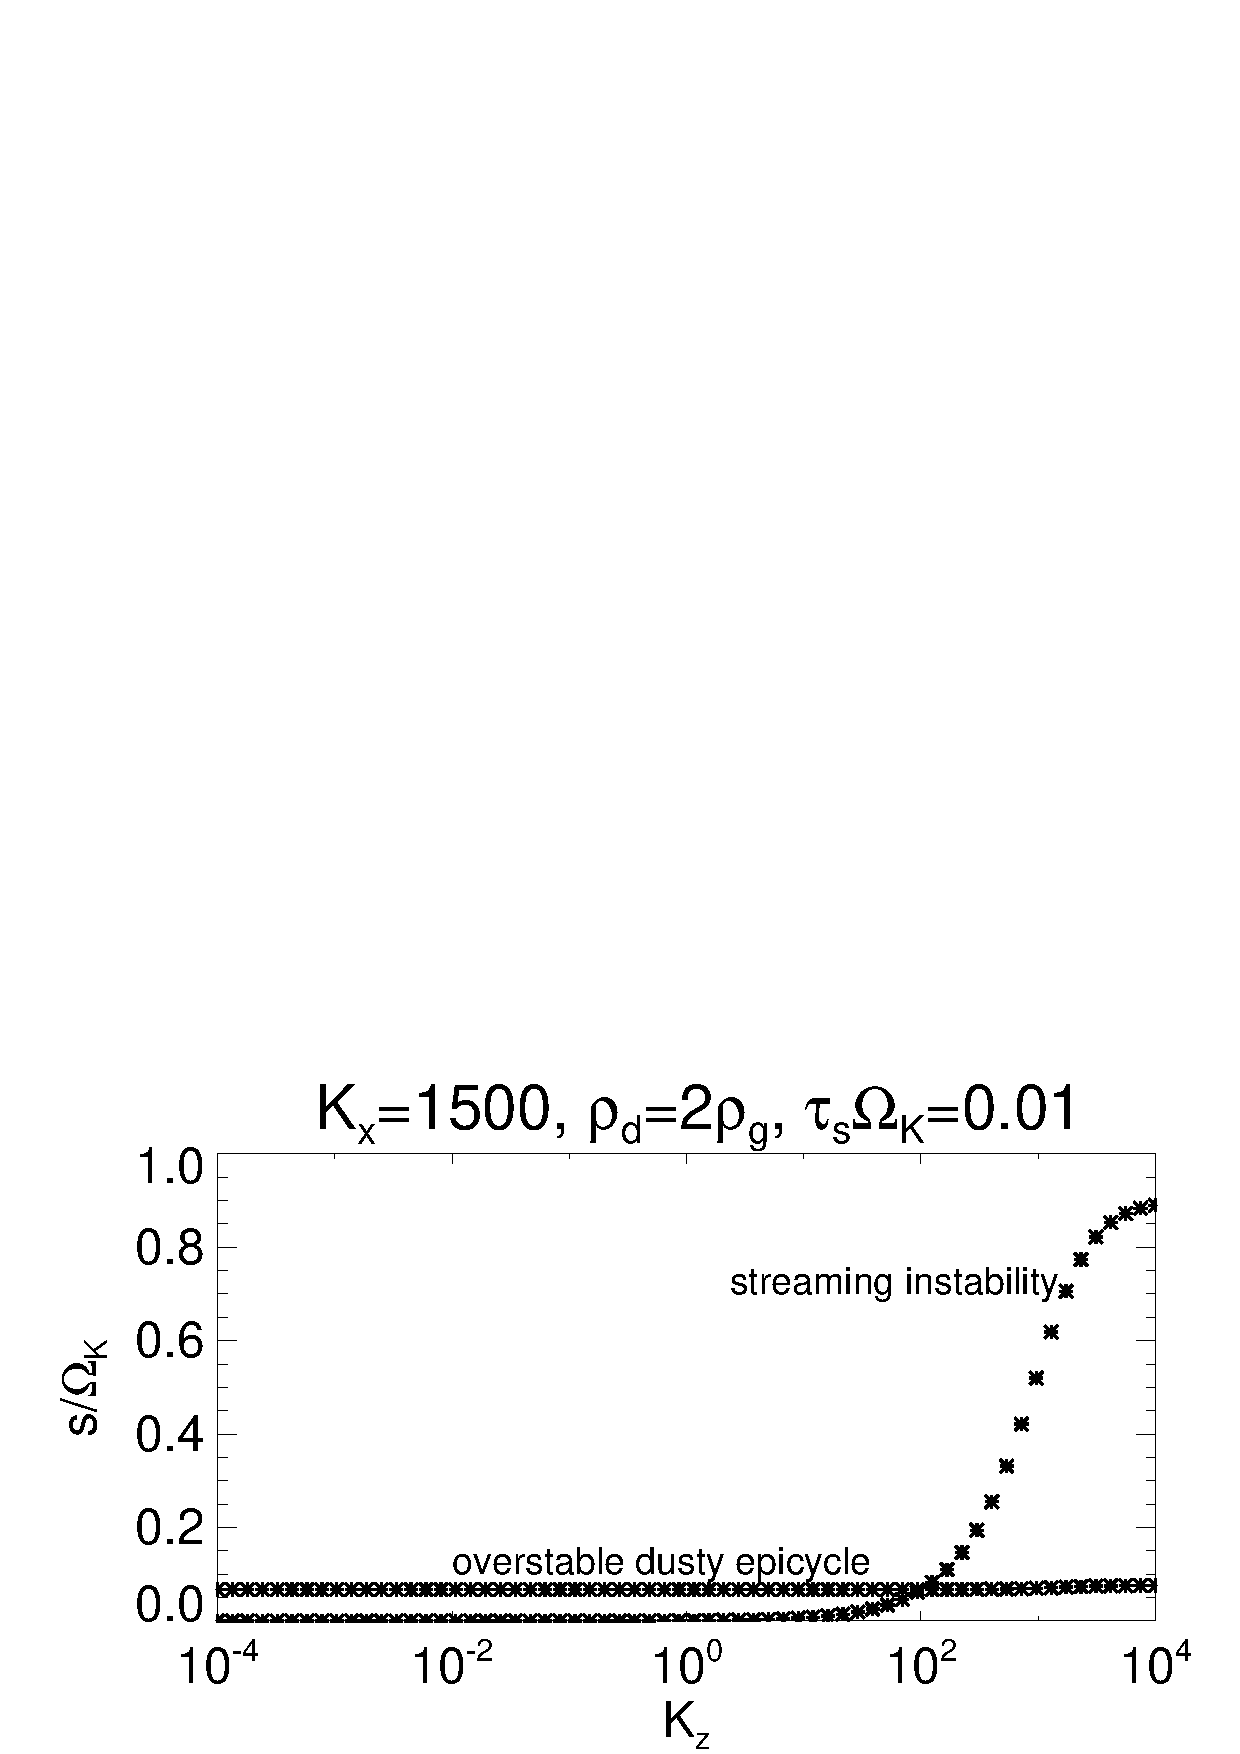
\includegraphics[width=\linewidth]{figures/streaming2}
  \caption{Growth rates of dust-drag instabilities with fixed radial
    wavenumber and dust-to-gas ratio, as a function of
    the vertical wavenumber at fix stopping time. \label{dusty_growth1}
  }
\end{figure}

Caution must be taken if the first-order one-fluid equations are used
to simulate dusty gas. 
%One should ensure that the physical dust-gas instabilty
%(which should have low-frequency in order for the first-order one-fluid
%approximation) has a larger growth rate than that of the spurious
%modes, which is given by Eq. \ref{epi_growth}. 
%Fig. \ref{dusty_growth1} suggests that the
%streaming instability would dominate, provided there is sufficient
%resolution to resolve high $K_z$ modes.  
For example, 2D, razor-thin disks would allow the spurious epicycles
to dominate, since in that case the streaming instability cannot
operate. Fig. \ref{dusty_growth1} suggest that in a realistic 3D disks
where a range of $K_z$ is allowed, the streaming instability should
dominate. 

Thus simulations based on the first-order one-fluid equations should
be set up to surpress these spurious epicycles. This might be
achieved, for example, through physical or numerical viscosity to
eliminate high-$k_x$ modes, since for fixed disk/dust parameters these
spurious epicycles only operate at sufficiently small radial
wavelengths. Alternatively, one needs to ensure the physical
instabilities of interest have larger growth rates than the spurious
epicycles. 


%An important caveat is that the one-fluid approximation for dusty gas 
%may not hold well when $|\omega| \gtrsim 
%\Omega$ \citep{youdin05a}, as is the case for dusty epicycles. 

% Their
% existence should be checked with full dust-plus-gas 
% simulations. Several 2D, razor-thin disk simulations do suggest a
% dusty instability that destory vortices
% \citep{fu14b,raettig15,surville16}. These setups are significantly
% more complex than our models, but \citeauthor{raettig15} did find 
% particle clumping in a test simulation without a vortex. These results
% might be related to the overstable dusty epicycles discussed here.       


% Real disks are three-dimensional, so the importance of dusty 
% epicycles should be compared with $k_z\neq0$ modes, which
% includes the classic streaming instability \citep{youdin05a},
% discussed next. 

%\subsection{Numerical example}


% In Fig. \ref{dusty_growth2} we fix the wavenumbers and vary the
% stopping time. The vertical dashed line is the critical stopping time
% for the overstable dusty epicycles, Eq. \ref{epi_grow_criterion},
% which is  
% \begin{align*}
%   \tau_{\mathrm{s,min}}\OmK = \frac{1}{2K_x\left(1-\tepsilon\right)^2} 
% \end{align*}
% in the above notation. For this example, $\tau_{\mathrm{s,min}}\OmK\simeq 
% 0.003$, as observed. On the other hand, the streaming instability
% shows weak dependence on $\taus$ for this range of stopping times 
% (it ultimated vanishes as $\taus\to0$). 

% \begin{figure}
%   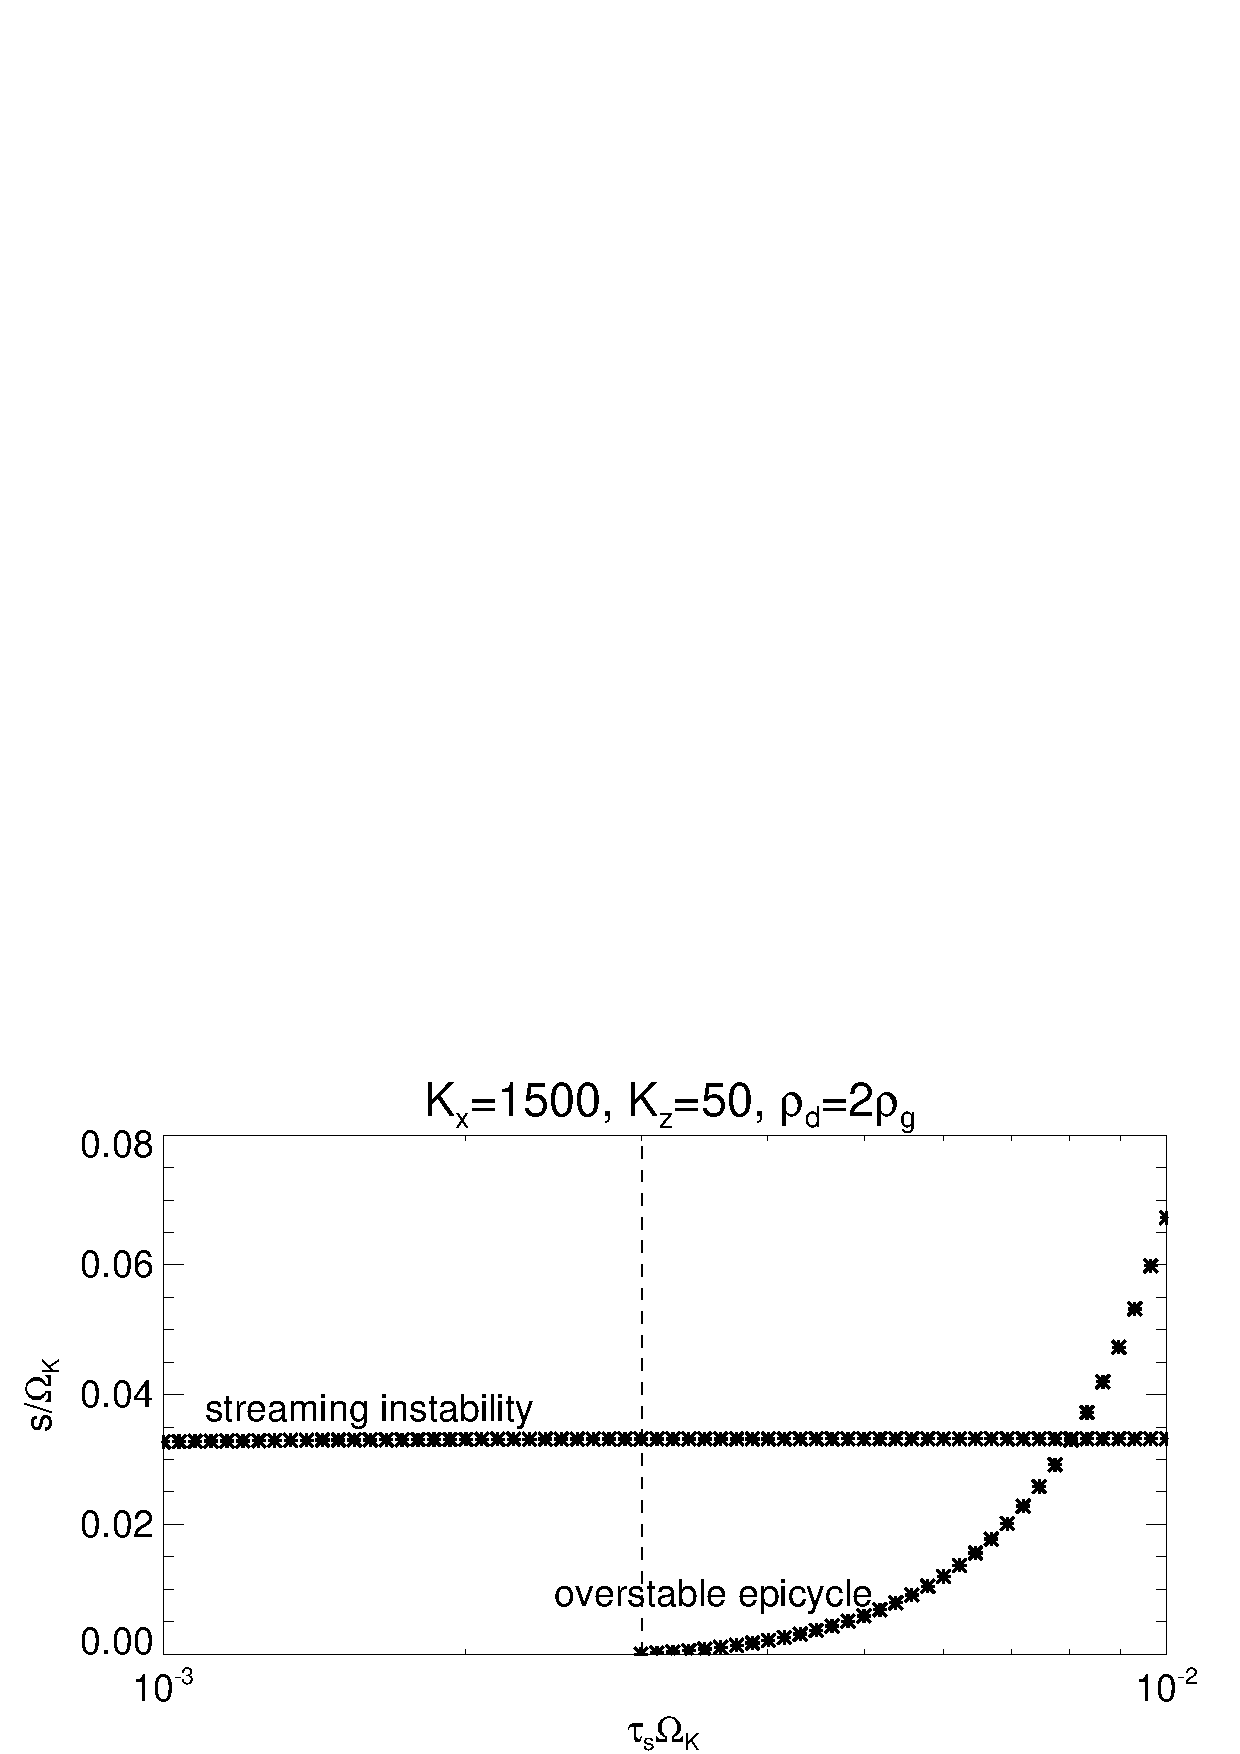
\includegraphics[width=\linewidth]{figures/streaming3}
%   \caption{Growth rates of dust-drag instabilities with fixed radial
%     wavenumber and dust-to-gas ratio, as a
%     function of stopping time at fixed vertical wavenumber. The
%     vertical dashed line correspond to the minimum stopping time for
%     growth of the dusty epicycle, given by
%     Eq. \protect\ref{epi_grow_criterion}. \label{dusty_growth2}
%   }
% \end{figure}

% These calculations suggest that in a realistic 3D dusty disk where
% vertical motions are allowed, the classic streaming
% instability is dominant because there exists $K_z$ values for which it
% dominates. This also renders the uncertainties in the  
% approximations used to describe the dusty epicycle modes
% irrelevant. On the other hand, the one-fluid framework can capture the
% streaming instability in the appropriate limit, as seen in Table
% \ref{si_compare}. 




%For small growth rates the real frequency $|\omega| =  
%O(\kappa)$, so these are overstable epicycles. 

%We finally note that Eq. \ref{epi_overs1}---\ref{epi_overs2} 
%admit pure oscillations with $s \equiv 0$, $\omega = 
%\pm\kappa$ if 
%\begin{align}
%  \tstop = \frac{\kappa}{k_x\left|F_r\right|}. 
%\end{align}
%This is the condition for marginal stability.  

% However, retaining all the terms (but still in the incompressible
% limit) can yield instability, as follows. Eq. \ref{kz_zero_si} admit
% pure oscillations with $\sigma = -\omega$ when 
% \begin{align*}
%   \omega &= \pm \kappa, \\
%   \tstop & = \frac{\omega}{ k _x F_r }
%          \equiv t_{\mathrm{s}0}.
% \end{align*} 
% Since $\tstop\geq 0$, we require $k_xF_r > 0$ if $\omega = \kappa$;
% and $k_xF_r < 0$ if $\omega = -\kappa$. For $k_x>0$ these marginally
% stable epicycles require radial pressure gradients decreasing and increasing
% outwards, respectively.  

%We require $\omega/k_xF_r> 0$  

% We now perturb about this state of marginal stability by writing
% $\sigma = \dd \sigma - \omega $ with $\dd\sigma = \ii\dd s -
% \dd\omega$, $\tstop = t_{\mathrm{s}0} +
% \dd\tstop $, and assume the $\dd$ quantities are small in
% magnitude. Then 
% \begin{align*} 
% \dd s = \frac{2\epsilon \kappa^2 }{1 +
%   4\epsilon^2 t_{\mathrm{s}0}^2\kappa^2}\dd \tstop. 
% \end{align*}
% Thus given $k_xF_r$, there exist growing modes 
% when the stopping time is slightly larger than
% $t_{\mathrm{s}0}$.  

% %{\bf note: several approx used}

% If we instead fix $\tstop$ and vary $k_xF_r$ about marginal stability,
% a similar exercise yields  
% \begin{align*} 
%   \dd s = \frac{\epsilon \tstop^3}{1 +
%   4\epsilon^2 \tstop^2 \kappa^2}\dd \left(k_x^2F_r^2\right).  
% \end{align*}
% Thus it is possible to destabilize the system by slightly increasing
% $|k_xF_r|>\kappa/ \tstop$ (i.e. shorter radial wavelengths and/or
% stronger pressure gradients).   



\bibliographystyle{apj}
\bibliography{ref}


\end{document}

